        %%******************************************%%
        %%                                          %%
        %%        Modello di tesi di laurea         %%
        %%            di Andrea Giraldin            %%
        %%                                          %%
        %%             2 novembre 2012              %%
        %%                                          %%
        %%******************************************%%


% I seguenti commenti speciali impostano:
% 1.
% 2. PDFLaTeX come motore di composizione;
% 3. tesi.tex come documento principale;
% 4. il controllo ortografico italiano per l'editor.

% !TEX encoding = UTF-8
% !TEX TS-program = pdflatex
% !TEX root = tesi.tex
% !TEX spellcheck = it-IT

\documentclass[10pt,                    % corpo del font principale
               a4paper,                 % carta A4
               twoside,                 % impagina per fronte-retro
               openright,               % inizio capitoli a destra
               english,
               italian,
               ]{book}

\usepackage[utf8]{inputenc}             % codifica di input; anche [latin1] va bene
                                        % NOTA BENE! va accordata con le preferenze dell'editor

%**************************************************************
% Importazione package
%**************************************************************

%\usepackage{amsmath,amssymb,amsthm}    % matematica

\usepackage[english, italian]{babel}    % per scrivere in italiano e in inglese;
                                        % l'ultima lingua (l'italiano) risulta predefinita

\usepackage{bookmark}                   % segnalibri

\usepackage{caption}                    % didascalie

\usepackage{chngpage,calc}              % centra il frontespizio

\usepackage{csquotes}                   % gestisce automaticamente i caratteri (")

\usepackage{emptypage}                  % pagine vuote senza testatina e piede di pagina

\usepackage{epigraph}					% per epigrafi

\usepackage{eurosym}                    % simbolo dell'euro

\usepackage[T1]{fontenc}                % codifica dei font:
                                        % NOTA BENE! richiede una distribuzione *completa* di LaTeX

%\usepackage{indentfirst}               % rientra il primo paragrafo di ogni sezione

\usepackage{graphicx}                   % immagini

\usepackage{hyperref}                   % collegamenti ipertestuali



\usepackage[binding=5mm]{layaureo}      % margini ottimizzati per l'A4; rilegatura di 5 mm

\usepackage{listings}                   % codici

\usepackage{microtype}                  % microtipografia

\usepackage{mparhack,fixltx2e,relsize}  % finezze tipografiche

\usepackage{nameref}                    % visualizza nome dei riferimenti

\usepackage[font=small]{quoting}        % citazioni

\usepackage{subfig}                     % sottofigure, sottotabelle

\usepackage[italian]{varioref}          % riferimenti completi della pagina

\usepackage[dvipsnames]{xcolor}         % colori

\usepackage{booktabs}                   % tabelle
\usepackage{tabularx}                   % tabelle di larghezza prefissata
\usepackage{longtable}                  % tabelle su più pagine
\usepackage{ltxtable}                   % tabelle su più pagine e adattabili in larghezza
\usepackage{float}

\usepackage[toc, acronym]{glossaries}   % glossario
                                        % per includerlo nel documento bisogna:
                                        % 1. compilare una prima volta tesi.tex;
                                        % 2. eseguire: makeindex -s tesi.ist -t tesi.glg -o tesi.gls tesi.glo
                                        % 3. eseguire: makeindex -s tesi.ist -t tesi.alg -o tesi.acr tesi.acn
                                        % 4. compilare due volte tesi.tex.

\usepackage[backend=biber,style=verbose-ibid,hyperref,backref]{biblatex}
                                        % eccellente pacchetto per la bibliografia;
                                        % produce uno stile di citazione autore-anno;
                                        % lo stile "numeric-comp" produce riferimenti numerici
                                        % per includerlo nel documento bisogna:
                                        % 1. compilare una prima volta tesi.tex;
                                        % 2. eseguire: biber tesi
                                        % 3. compilare ancora tesi.tex.

\usepackage{enumitem}

\usepackage{multirow}

%**************************************************************
% file contenente le impostazioni della tesi
%**************************************************************

%**************************************************************
% Frontespizio
%**************************************************************

% Autore
\newcommand{\myName}{Nicola Dal Maso}
\newcommand{\myTitle}{Un prototipo di sistema di Home Automation basato su microservizi}

% Tipo di tesi
\newcommand{\myDegree}{Tesi di laurea triennale}

% Università
\newcommand{\myUni}{Università degli Studi di Padova}

% Facoltà
\newcommand{\myFaculty}{Corso di Laurea in Informatica}

% Dipartimento
\newcommand{\myDepartment}{Dipartimento di Matematica "Tullio Levi-Civita"}

% Titolo del relatore
\newcommand{\profTitle}{Prof. }

% Relatore
\newcommand{\myProf}{Tullio Vardanega}

% Luogo
\newcommand{\myLocation}{Padova}

% Anno accademico
\newcommand{\myAA}{2017-2018}

% Data discussione
\newcommand{\myTime}{Febbraio 2018}

% checkmark
\newcommand{\cmark}{\ding{51}}%

% non checkmark
\newcommand{\xmark}{\ding{55}}%


%**************************************************************
% Impostazioni di impaginazione
% see: http://wwwcdf.pd.infn.it/AppuntiLinux/a2547.htm
%**************************************************************

\setlength{\parindent}{14pt}   % larghezza rientro della prima riga
\setlength{\parskip}{0pt}   % distanza tra i paragrafi


%**************************************************************
% Impostazioni di biblatex
%**************************************************************
\bibliography{bibliografia} % database di biblatex

\defbibheading{bibliography} {
    \cleardoublepage
    \phantomsection
    \addcontentsline{toc}{chapter}{\bibname}
    \chapter*{\bibname\markboth{\bibname}{\bibname}}
}

\setlength\bibitemsep{1.5\itemsep} % spazio tra entry

\DeclareBibliographyCategory{opere}
\DeclareBibliographyCategory{web}

\addtocategory{opere}{womak:lean-thinking}
\addtocategory{web}{site:agile-manifesto}

\defbibheading{opere}{\section*{Riferimenti bibliografici}}
\defbibheading{web}{\section*{Siti Web consultati}}


%**************************************************************
% Impostazioni di caption
%**************************************************************
\captionsetup{
    tableposition=top,
    figureposition=bottom,
    font=small,
    format=hang,
    labelfont=bf
}

%**************************************************************
% Impostazioni di glossaries
%**************************************************************
\renewcommand{\glstextformat}[1]{#1\glsfirstoccur}

%**************************************************************
% Acronimi
%**************************************************************
\renewcommand{\acronymname}{Acronimi e abbreviazioni}

\newacronym[description={\glslink{apig}{Application Program Interface}}]
    {api}{API}{Application Program Interface}

\newacronym[description={\glslink{umlg}{Unified Modeling Language}}]
    {uml}{UML}{Unified Modeling Language}

\newacronym{mit-acronym}{MIT}{Massachusetts Institute of Technology}

\newacronym{cli-acronym}{CLI}{Command Line Interface}

\newacronym{cpu-acronym}{CPU}{Central Processing Unit}

\newacronym{gpu-acronym}{GPU}{Graphics Processing Unit}

\newacronym{ide-acronym}{IDE}{Integrated Development Environment}

\newacronym{dom-acronym}{DOM}{Document Object Model}

\newacronym{qos-acronym}{QoS}{Quality of Service}

\newacronym{mqtt-acronym}{MQTT}{MQ Telemetry Transport}

%**************************************************************
% Glossario
%**************************************************************
\renewcommand{\glossaryname}{Glossario}

\newglossaryentry{apig}
{
    name=\glslink{api}{API},
    text=\emph{Application Program Interface},
    sort=api,
    description={in informatica con il termine \emph{Application Programming Interface API} (ing. interfaccia di programmazione di un'applicazione) si indica ogni insieme di procedure disponibili al programmatore, di solito raggruppate a formare un set di strumenti specifici per l'espletamento di un determinato compito all'interno di un certo programma. La finalità è ottenere un'astrazione, di solito tra l'hardware e il programmatore o tra software a basso e quello ad alto livello semplificando così il lavoro di programmazione}
}

\newglossaryentry{umlg}
{
    name=\glslink{uml}{UML},
    text=UML,
    sort=uml,
    description={in ingegneria del software \emph{UML, Unified Modeling Language} (ing. linguaggio di modellazione unificato) è un linguaggio di modellazione e specifica basato sul paradigma object-oriented. L'\emph{UML} svolge un'importantissima funzione di ``lingua franca'' nella comunità della progettazione e programmazione a oggetti. Gran parte della letteratura di settore usa tale linguaggio per descrivere soluzioni analitiche e progettuali in modo sintetico e comprensibile a un vasto pubblico}
}

\newglossaryentry{load balancerg}
{
  name=\emph{Load balancer},
  text=load balancer,
  sort=load balancer,
  description={in informatica, il load balancer è lo strumento hardware o software attraverso cui viene distribuito un carico di lavoro su più risorse di elaborazione (\textit{load balancing})}
}

\newglossaryentry{throughputg}
{
  name=\emph{Throughput},
  text=throughput,
  sort=throughput,
  description={indica la capacità di un canale di comunicazione di processare o trasmettere dati in uno specifico periodo di tempo. É una misura di produttività.}
}

\newglossaryentry{aspettativag}
{
  name=Aspettativa,
  text=aspettativa,
  sort=aspettativa,
  description={è un periodo di astensione dal lavoro, previsto dalla legge, che il datore di lavoro può concedere ad un proprio lavoratore per motivi familiari o personali, generalmente non retribuito}
}

\newglossaryentry{kernelg}
{
  name=\emph{Kernel},
  text={Kernel},
  sort=kernel,
  description={è il sottosistema di un sistema operativo che fornisce ai processi in esecuzione sull'elaboratore l'accesso alle risorse fisiche, in modo controllato e sicuro}
}

\newglossaryentry{MIT}
{
  name=\gls{mit-acronym},
  text=MIT,
  sort=mit,
  description={nell'ambito delle licenze \emph{software}, la licenza MIT è una licenza creata dal \emph{Massachusetts Institute of Technology} per il rilascio di codice sorgente secondo condizioni permissive da parte dell'utilizzatore del codice, tutelando il \emph{copyright} dell'autore}
}

\newglossaryentry{broadcast}
{
  name=\emph{Broadcast},
  text={Broadcast},
  sort=broadcast,
  description={nell'ambito delle telecomunicazione, indica una trasmissione delle informazioni da un sistema trasmittente ad un insieme di apparati riceventi non conosciuto a priori (uno a molti)}
}

\newglossaryentry{pattern}
{
  name=\emph{Pattern},
  text={Pattern},
  sort=pattern,
  description={in informatica è una soluzione testata e dimostrata ad un problema ricorrente. La sua accezione principale consiste in quella di \emph{Design Pattern} (soluzioni progettuali)}
}

\newglossaryentry{Gatewaypattern}
{
  name=\emph{Gateway Pattern},
  text={Gateway Pattern},
  sort=gateway pattern,
  description={è un \gls{pattern} che propone una soluzione al problema "Come un \emph{client} può interagire con un sistema a microservizi?". Questo è un peculiare problema delle architetture a microservizi e la soluzione proposta consiste nel sviluppare un servizio la cui funzionalità principale consiste nel gestire le richieste dei \emph{client} in un singolo \emph{entrypoint} pubblico, che si occupa di redirezionare la richiesta al servizio adeguato o assembla una risposta complessa a partire dalle informazioni messe a disposizione da più servizi\footcite{gateway-pattern}}
}

\newglossaryentry{js}
{
  name=\emph{JavaScript},
  text={JavaScript},
  sort={javascript},
  description={è un linguaggio di programmazione nato per aggiungere dinamicità e interattività alle pagine renderizzate dai browser attraverso l'esecuzione di semplici istruzioni che manipolino la struttura della pagina \emph{web} visualizzata}
}

\newglossaryentry{broker}
{
  name=\emph{Broker},
  text={broker},
  sort={broker},
  description={un broker nell'ambito MQTT è un server che reindirizza i messaggi pubblicati verso i client sottoscritti all'argomento di ciascun messaggio}
}

\newglossaryentry{milestone}
{
  name=\emph{Milestone},
  text={milestone},
  sort={milestone},
  description={nell'ambito della pianificazione di un progetto, indica il raggiungimento di obiettivi stabiliti in fase di definizione del progetto}
}

\newglossaryentry{open source}
{
  name=\emph{Open source},
  text={open source},
  sort={open source},
  description={indica un prodotto \emph{software} in cui il codice sorgente è pubblicato dagli autori al fine di favorirne lo studio, aumentarne la diffusione e permettere alla comunità di apportarvi modifiche}
}

\newglossaryentry{CLI}
{
  name=\gls{cli-acronym},
  text=CLI,
  sort=cli,
  description={indica un'interfaccia utente in cui l'interazione avviene attraverso la digitazione di comandi testuali}
}

\newglossaryentry{CPU}
{
  name=\gls{cpu-acronym},
  text=CPU,
  sort=cpu,
  description={è un tipo di dispositivo \emph{hardware} dedicato all'esecuzione di istruzioni generiche definite in un insieme di istruzioni eseguibili (\emph{instruction set})}
}

\newglossaryentry{GPU}
{
  name=\gls{gpu-acronym},
  text=GPU,
  sort=gpu,
  description={è un tipo di dispositivo \emph{hardware} specializzato nell'esecuzione di istruzioni per la visualizzazione delle immagini a schermo}
}

\newglossaryentry{mocking}
{
  name=\emph{Mock},
  text=mock,
  sort=mock,
  description={nell'ambito della programmazione ad oggetti, indica un oggetto che simula il comportamento di un altro oggetto non accessibile o non implementato. I \emph{mock} sono utilizzati principalmente per isolare un oggetto dalle sue dipendenze durante le attività di test}
}

\newglossaryentry{IDE}
{
  name=\gls{ide-acronym},
  text=IDE,
  sort=ide,
  description={è un \emph{software} che aiuta gli sviluppatori nella scrittura del codice sorgente di un programma, segnalando errori di sintassi e fornendo funzionalità per l'ispezione del codice alla ricerca di errori}
}

\newglossaryentry{Google}
{
  name=Google,
  text=Google,
  sort=google,
  description={è un'azienda statunitense che opera nel campo dei servizi \emph{online} e della telefonia (attraverso il sistema operativo Android)}
}

\newglossaryentry{Microsoft}
{
  name=Microsoft,
  text=Microsoft,
  sort=microsoft,
  description={è un'azienda statunitense che opera nel campo dell'informatica, sviluppando sistemi operativi, \emph{software} per la produttività aziendale e domestica ed elettronica di consumo}
}

\newglossaryentry{GitHub}
{
  name=GitHub,
  text=GitHub,
  sort=github,
  description={è un servizio che permette di mantenere documenti e progetti \emph{software} all'interno di un controllo di versione distribuito. Il servizio è sviluppato dall'omonima azienda}
}

\newglossaryentry{DOM}
{
  name=\gls{dom-acronym},
  text=DOM,
  sort=dom,
  description={è una forma di rappresentazione per documenti strutturati utilizzando modelli orientati agli oggetti}
}

\newglossaryentry{CPU-bound}
{
  name=\emph{CPU-bound},
  text=CPU-bound,
  sort=cpu-bound,
  description={l'espressione indica quei processi che sfruttano le risorse di elaborazione di una CPU, ma non richiedono servizi di scambio dati con l'esterno. Un esempio di \emph{software} tipicamente \emph{CPU-bound} riguarda i programmi di calcolo matematico}
}

\newglossaryentry{overhead}
{
  name=\emph{Overhead},
  text=overhead,
  sort=overhead,
  description={indica le risorse richieste in più rispetto a quelle necessarie per ottenere un determinato scopo}
}

\newglossaryentry{QoS}
{
  name=\gls{qos-acronym},
  text=QoS,
  sort=qos,
  description={nell'ambito delle reti di telecomunicazioni, il QoS indica i parametri usati per qualificare le prestazioni e l'affidabilità di un servizio offerto dalla rete}
}

\newglossaryentry{handshake}
{
  name=\emph{Handshake},
  text=handshake,
  sort=handshake,
  description={in informatica rappresenta il processo attraverso cui due elaboratori stabiliscono un insieme di regole comuni per la comunicazione di dati}
}

\newglossaryentry{MQTT}
{
  name=\gls{mqtt-acronym},
  text=MQTT,
  sort=mqtt,
  description={è un protocollo di comunicazione leggero basato sullo scambio di messaggi tra dispositivi caratterizzati da risorse di elaborazione limitate in una rete inaffidabile}
}

\newglossaryentry{abstract-factory}
{
  name=\emph{Abstract Factory},
  text=Abstract Factory,
  sort=abstract factory,
  description={è un \gls{pattern} creazionale che fornisce un'interfaccia per creare famiglie di oggetti connessi o dipendenti tra loro, in modo che non ci sia necessità da parte dei \emph{client} di specificare quale classe istanziare. Questo pattern permette che un sistema sia indipendente dall'implementazione degli oggetti concreti e che il \emph{client}, attraverso l'interfaccia, utilizzi diverse famiglie di prodotti}
}

\newglossaryentry{WebSocket}
{
  name=\emph{WebSocket},
  text=WebSocket,
  sort=websocket,
  description={è una tecnologia che fornisce canali di comunicazione in cui le informazioni viaggiano sia dal \emph{client} al server che viceversa e permette di realizzare applicazioni \emph{web} in cui vi è comunicazione in tempo reale tra il server e il \emph{client}}
}

\newglossaryentry{dp-composite}
{
  name=\emph{Composite},
  text=Composite,
  sort=composite,
  description={è un \gls{pattern} strutturale che permette di effettuare operazioni su gruppi di oggetti come se essi fossero l'istanza di un singolo oggetto e permette di manipolare oggetti singoli e loro composizioni in modo uniforme}
}

\newglossaryentry{repository}
{
  name=\emph{Repository},
  text=repository,
  sort=repository,
  description={è un sistema \emph{software} che archivia un insieme di \emph{file} e cartelle e le relative informazioni al fine di permettere la distribuzione sicura e affidabile di questo insieme di dati}
}

\newglossaryentry{sharding}
{
  name=\emph{Sharding},
  text=sharding,
  sort=sharding,
  description={nell'ambito delle tecnologie per i \emph{database}, è il procedimento attraverso cui un \emph{database} principale partiziona i dati ricevuti su molteplici istanze del \emph{database}, definite \emph{slave}. I dati in una architettura di questo tipo sono frammentati tra \emph{database} separati, potenzialmente aumentando le prestazioni e la resilienza dei dati}
}

\newglossaryentry{callback}
{
  name=\emph{Callback},
  text=Callback,
  sort=callback,
  description={è un \gls{pattern} che permette di delegare l'esecuzione di una funzione, passandola in \emph{input} di un'altra funzione. Le funzioni di \emph{callback} sono invocate per propagare i risultati di un'operazione complessa attraverso diversi \emph{step}.}
}
 % database di termini
\makeglossaries


%**************************************************************
% Impostazioni di graphicx
%**************************************************************
\graphicspath{{immagini/}} % cartella dove sono riposte le immagini


%**************************************************************
% Impostazioni di hyperref
%**************************************************************
\hypersetup{
    %hyperfootnotes=false,
    %pdfpagelabels,
    %draft,	% = elimina tutti i link (utile per stampe in bianco e nero)
    colorlinks=true,
    linktocpage=true,
    pdfstartpage=1,
    pdfstartview=FitV,
    % decommenta la riga seguente per avere link in nero (per esempio per la stampa in bianco e nero)
    %colorlinks=false, linktocpage=false, pdfborder={0 0 0}, pdfstartpage=1, pdfstartview=FitV,
    breaklinks=true,
    pdfpagemode=UseNone,
    pageanchor=true,
    pdfpagemode=UseOutlines,
    plainpages=false,
    bookmarksnumbered,
    bookmarksopen=true,
    bookmarksopenlevel=1,
    hypertexnames=true,
    pdfhighlight=/O,
    %nesting=true,
    %frenchlinks,
    urlcolor=webbrown,
    linkcolor=RoyalBlue,
    citecolor=webgreen,
    %pagecolor=RoyalBlue,
    %urlcolor=Black, linkcolor=Black, citecolor=Black, %pagecolor=Black,
    pdftitle={\myTitle},
    pdfauthor={\textcopyright\ \myName, \myUni, \myFaculty},
    pdfsubject={},
    pdfkeywords={},
    pdfcreator={pdfLaTeX},
    pdfproducer={LaTeX}
}

%**************************************************************
% Impostazioni di itemize
%**************************************************************
\renewcommand{\labelitemi}{$\bullet$}

%\renewcommand{\labelitemi}{$\bullet$}
%\renewcommand{\labelitemii}{$\cdot$}
%\renewcommand{\labelitemiii}{$\diamond$}
%\renewcommand{\labelitemiv}{$\ast$}


%**************************************************************
% Impostazioni di listings
%**************************************************************
\lstset{
    language=[LaTeX]Tex,%C++,
    keywordstyle=\color{RoyalBlue}, %\bfseries,
    basicstyle=\small\ttfamily,
    %identifierstyle=\color{NavyBlue},
    commentstyle=\color{Green}\ttfamily,
    stringstyle=\rmfamily,
    numbers=none, %left,%
    numberstyle=\scriptsize, %\tiny
    stepnumber=5,
    numbersep=8pt,
    showstringspaces=false,
    breaklines=true,
    frameround=ftff,
    frame=single
}


%**************************************************************
% Impostazioni di xcolor
%**************************************************************
\definecolor{webgreen}{rgb}{0,.5,0}
\definecolor{webbrown}{rgb}{.6,0,0}


%**************************************************************
% Altro
%**************************************************************

\newcommand{\omissis}{[\dots\negthinspace]} % produce [...]

% eccezioni all'algoritmo di sillabazione
\hyphenation
{
    ma-cro-istru-zio-ne
    gi-ral-din
}

\newcommand{\sectionname}{sezione}
\addto\captionsitalian{\renewcommand{\figurename}{Figura}
                       \renewcommand{\tablename}{Tabella}}

\newcommand{\glsfirstoccur}{\ap{{[g]}}}

\newcommand{\intro}[1]{\emph{\textsf{#1}}}

%**************************************************************
% Environment per ``rischi''
%**************************************************************
\newcounter{riskcounter}                % define a counter
\setcounter{riskcounter}{0}             % set the counter to some initial value

%%%% Parameters
% #1: Title
\newenvironment{risk}[1]{
    \refstepcounter{riskcounter}        % increment counter
    \par \noindent                      % start new paragraph
    \textbf{\arabic{riskcounter}. #1}   % display the title before the
                                        % content of the environment is displayed
}{
    \par\medskip
}

\newcommand{\riskname}{Rischio}

\newcommand{\riskdescription}[1]{\textbf{\\Descrizione:} #1.}

\newcommand{\risksolution}[1]{\textbf{\\Soluzione:} #1.}

%**************************************************************
% Environment per ``use case''
%**************************************************************
\newcounter{usecasecounter}             % define a counter
\setcounter{usecasecounter}{0}          % set the counter to some initial value

%%%% Parameters
% #1: ID
% #2: Nome
\newenvironment{usecase}[2]{
    \renewcommand{\theusecasecounter}{\usecasename #1}  % this is where the display of
                                                        % the counter is overwritten/modified
    \refstepcounter{usecasecounter}             % increment counter
    \vspace{10pt}
    \par \noindent                              % start new paragraph
    {\large \textbf{\usecasename #1: #2}}       % display the title before the
                                                % content of the environment is displayed
    \medskip
}{
    \medskip
}

\newcommand{\usecasename}{UC}

\newcommand{\usecaseactors}[1]{\textbf{\\Attori Principali:} #1. \vspace{4pt}}
\newcommand{\usecasepre}[1]{\textbf{\\Precondizioni:} #1. \vspace{4pt}}
\newcommand{\usecasedesc}[1]{\textbf{\\Descrizione:} #1. \vspace{4pt}}
\newcommand{\usecasepost}[1]{\textbf{\\Postcondizioni:} #1. \vspace{4pt}}
\newcommand{\usecasealt}[1]{\textbf{\\Scenario Alternativo:} #1. \vspace{4pt}}

%**************************************************************
% Environment per ``namespace description''
%**************************************************************

\newenvironment{namespacedesc}{
    \vspace{10pt}
    \par \noindent                              % start new paragraph
    \begin{description}
}{
    \end{description}
    \medskip
}

\newcommand{\classdesc}[2]{\item[\textbf{#1:}] #2}
                     % file con le impostazioni personali

\begin{document}
%**************************************************************
% Materiale iniziale
%**************************************************************
\frontmatter
% !TEX encoding = UTF-8
% !TEX TS-program = pdflatex
% !TEX root = ../relazione-finale.tex

%**************************************************************
% Frontespizio 
%**************************************************************
\begin{titlepage}

\begin{center}

\begin{LARGE}
\textbf{\myUni}\\
\end{LARGE}

\vspace{10pt}

\begin{Large}
\textsc{\myDepartment}\\
\end{Large}

\vspace{10pt}

\begin{large}
\textsc{\myFaculty}\\
\end{large}

\vspace{30pt}
\begin{figure}[htbp]
\begin{center}
\includegraphics[height=6cm]{logo-unipd}
\end{center}
\end{figure}
\vspace{30pt} 

\begin{LARGE}
\begin{center}
\textbf{\myTitle}\\
\end{center}
\end{LARGE}

\vspace{10pt} 

\begin{large}
\textsl{\myDegree}\\
\end{large}

\vspace{40pt} 

\begin{large}
\begin{flushleft}
\textit{Relatore}\\ 
\vspace{5pt} 
\profTitle \myProf
\end{flushleft}

\vspace{0pt} 

\begin{flushright}
\textit{Laureando}\\ 
\vspace{5pt} 
\myName
\end{flushright}
\end{large}

\vspace{40pt}

\line(1, 0){338} \\
\begin{normalsize}
\textsc{Anno Accademico \myAA}
\end{normalsize}

\end{center}
\end{titlepage} 
% % !TEX encoding = UTF-8
% !TEX TS-program = pdflatex
% !TEX root = ../relazione-finale.tex

%**************************************************************
% Colophon
%**************************************************************
\clearpage
\phantomsection
\thispagestyle{empty}

\hfill

\vfill

\noindent\myName: \textit{\myTitle,}
\myDegree,
\textcopyright\ \myTime.
% !TEX encoding = UTF-8
% !TEX TS-program = pdflatex
% !TEX root = ../relazione-finale.tex

%**************************************************************
% Dedica
%**************************************************************
\cleardoublepage
\phantomsection
\thispagestyle{empty}
\pdfbookmark{Dedica}{Dedica}

\vspace*{3cm}

\begin{center}
Lorem ipsum dolor sit amet, consectetuer adipiscing elit. \\ \medskip
--- Oscar Wilde    
\end{center}

\medskip

\begin{center}
Dedicato a ...
\end{center}

% !TEX encoding = UTF-8
% !TEX TS-program = pdflatex
% !TEX root = ../relazione-finale.tex

%**************************************************************
% Sommario
%**************************************************************
\cleardoublepage
\phantomsection
\pdfbookmark{Sommario}{Sommario}
\begingroup
\let\clearpage\relax
\let\cleardoublepage\relax
\let\cleardoublepage\relax

\chapter*{Sommario}

Il presente documento descrive il lavoro svolto durante il periodo di stage, della durata di circa trecento ore, dal laureando Pinco Pallino presso l'azienda Azienda S.p.A.
Gli obbiettivi da raggiungere erano molteplici.\\
In primo luogo era richiesto lo sviluppo di ...
In secondo luogo era richiesta l'implementazione di un ... 
Tale framework permette di registrare gli eventi di un controllore programmabile, quali segnali applicati 
Terzo ed ultimo obbiettivo era l'integrazione ...

%\vfill
%
%\selectlanguage{english}
%\pdfbookmark{Abstract}{Abstract}
%\chapter*{Abstract}
%
%\selectlanguage{italian}

\endgroup			

\vfill


% !TEX encoding = UTF-8
% !TEX TS-program = pdflatex
% !TEX root = ../relazione-finale.tex

%**************************************************************
% Ringraziamenti
%**************************************************************
\cleardoublepage
\phantomsection
\pdfbookmark{Ringraziamenti}{ringraziamenti}

\begin{flushright}{
	\slshape    
	``Life is really simple, but we insist on making it complicated''} \\ 
	\medskip
    --- Confucius
\end{flushright}


\bigskip

\begingroup
\let\clearpage\relax
\let\cleardoublepage\relax
\let\cleardoublepage\relax

\chapter*{Ringraziamenti}

\noindent \textit{Innanzitutto, vorrei esprimere la mia gratitudine al Prof. NomeDelProfessore, relatore della mia tesi, per l'aiuto e il sostegno fornitomi durante la stesura del lavoro.}\\

\noindent \textit{Desidero ringraziare con affetto i miei genitori per il sostegno, il grande aiuto e per essermi stati vicini in ogni momento durante gli anni di studio.}\\

\noindent \textit{Ho desiderio di ringraziare poi i miei amici per tutti i bellissimi anni passati insieme e le mille avventure vissute.}\\
\bigskip

\noindent\textit{\myLocation, \myTime}
\hfill \myName

\endgroup


% !TEX encoding = UTF-8
% !TEX TS-program = pdflatex
% !TEX root = ../relazione-finale.tex

%**************************************************************
% Convenzioni tipografiche
%**************************************************************
\cleardoublepage
\phantomsection
\thispagestyle{empty}
\pdfbookmark{Convenzioni tipografiche}{Convenzioni tipografiche}

\vspace*{3cm}

\chapter*{Convenzioni tipografiche}

Riguardo la stesura del testo, relativamente al documento sono state adottate le seguenti convenzioni tipografiche:
\begin{itemize}
	\item gli acronimi, le abbreviazioni e i termini ambigui o di uso non comune menzionati vengono definiti nel glossario, situato alla fine del presente documento;
	\item per la prima occorrenza dei termini riportati nel glossario viene utilizzata la seguente nomenclatura: \emph{parola}\glsfirstoccur;
	\item i termini in lingua straniera o facenti parti del gergo tecnico sono evidenziati con il carattere \emph{corsivo}.
\end{itemize}
% !TEX encoding = UTF-8
% !TEX TS-program = pdflatex
% !TEX root = ../relazione-finale.tex

%**************************************************************
% Indici
%**************************************************************
\cleardoublepage
\pdfbookmark{\contentsname}{tableofcontents}
\setcounter{tocdepth}{2}
\tableofcontents
%\markboth{\contentsname}{\contentsname} 
\clearpage

\begingroup 
    \let\clearpage\relax
    \let\cleardoublepage\relax
    \let\cleardoublepage\relax
    %*******************************************************
    % Elenco delle figure
    %*******************************************************    
    \phantomsection
    \pdfbookmark{\listfigurename}{lof}
    \listoffigures

    \vspace*{8ex}

    %*******************************************************
    % Elenco delle tabelle
    %*******************************************************
    \phantomsection
    \pdfbookmark{\listtablename}{lot}
    \listoftables
        
    \vspace*{8ex}
\endgroup

\cleardoublepage

\cleardoublepage

%**************************************************************
% Materiale principale
%**************************************************************
\mainmatter
% !TEX encoding = UTF-8
% !TEX TS-program = pdflatex
% !TEX root = ../relazione-finale.tex

%**************************************************************
\chapter{Introduzione}
\label{cap:introduzione}
%**************************************************************

% \noindent Esempio di utilizzo di un termine nel glossario \\
% \gls{api}. \\
%
% \noindent Esempio di citazione in linea \\
% \cite{site:agile-manifesto}. \\
%
% \noindent Esempio di citazione nel pie' di pagina \\
% citazione\footcite{womak:lean-thinking} \\

%**************************************************************
\section{L'idea}

% obiettivi dello stage

% caratteristiche dello stage

In questa relazione descrivo lo svolgimento dello stage effettuato nel contesto del Corso di Laurea di Informatica dell'Università di Padova.

Ho intrapreso lo stage nella sua forma interna individuale, in cui con il proponente, \profTitle \myProf, ho redatto un piano di lavoro nel quale lo stage abbia una durata pianificata su 300 ore.

L'obiettivo principale dello stage consiste nello sviluppo e nella realizzazione di un prototipo per la gestione di dispositivi interconnessi (IoT) attraverso un'interfaccia \emph{web}.
Questo centro di controllo attraverso cui l'utente del sistema gestisce i dispositivi \emph{smart} presenti nella propria rete domestica dovrebbe permettere operazioni quali:
\begin{itemize}
  \item avvio/spegnimento di un dispositivo;
  \item monitoraggio dei dispositivi collegati;
  \item collegamento all'eventuale interfaccia proprietaria del dispositivo (es. supporto tecnico).
\end{itemize}

Ho sviluppato e realizzato il progetto di stage con l'idea di unificare in un unico centro di controllo tutti gli eventuali dispositivi connessi alla rete domestica dell'utente, permettendo tuttavia allo stesso di accedere all'interfaccia proprietaria di ciascun dispositivo.
L'obiettivo di una tale \emph{dashboard} non è quindi confinare l'utente in un unico ecosistema domotico,
bensì quello di facilitare la consultazione delle informazioni più frequentemente richieste dall'utente provenienti da più ecosistemi distinti. \\
Grazie alla natura prototipale del prodotto sviluppato, ho inoltre potuto sperimentare l'approccio architetturale a microservizi, al fine di garantire scalabilità all'applicazione.

%**************************************************************
\section{IoT: definizione e caratteristiche generali}
\label{intro-iot}

\emph{Internet Of Things} è un paradigma tecnologico diffusosi nell'ultimo decennio. Questa locuzione fa riferimento a un insieme di oggetti,
di varia natura e utilizzo, che interagiscono tra loro e che permettono all'utente di interagire con essi. \\ \\

Un dispositivo \emph{smart} è un dispositivo elettronico, generalmente connesso ad altri dispositivi, che può svolgere le proprie funzioni in maniera autonoma.
Un esempio lampante di dispositivi \emph{smart} sono gli smartphone, prodotti che hanno arricchito di funzionalità avanzate, interagendo con l'utente in modi precedentemente non possibili, i predecessori telefoni (\emph{phone}).
\footcite{site:smart-device}

Studenti e professori del Dipartimento di Informatica dell'Università di Carnegie Mellon presero in considerazione l'idea di una rete di dispositivi \emph{smart} quando modificarono un distributore automatico di bibite del Dipartimento per accedere al suo inventario di bibite. Quel distributore automatico divenne il primo apparecchio collegato ad Internet.
\footcite{site:mellon-uni}

Nel corso degli anni '90 il mondo accademico e il mondo dell'industra legata alla produzione continuarono a sperimentare evolvendo il \textit{concept} iniziale, arrivando alla conclusione che l'\textit{Ubiquitous Computing} non si debba riferire solamente ai \textit{computer}, ma debba espandersi agli oggetti di utilizzo quotidiano. Questa visione dovette scontrarsi con i limiti della microelettronica di allora: la produzione di semiconduttori non era ancora pronta a supportare la potenziale domanda e i costi per sostenere l'ampliamento degli impianti non erano facilmente assorbibili in breve tempo.
\footcite{site:mit-weiser}

Kevin Ashton coniò il termine \textit{"Internet of Things"} nel 1999.
\footcite{site:iot-kashton}
L'origine dell'espressione, riassumendo le parole dell'autore, deriva dal fatto che la maggior parte delle informazioni presenti su Internet sono state e sono inserite da utenti "umani", soggetti quindi a concentrazione, precisione e tempo limitate;
se queste informazioni fossero invece inserite da macchine senza l'aiuto di un utente umano, la maggior qualità delle stesse garantirebbe:
\setlist{nolistsep}
\begin{itemize}
  \item maggiore capacità di tracciamento delle risorse;
  \item minor spreco di risorse;
  \item minor costo per la gestione delle risorse.
\end{itemize}

Grazie agli avanzamenti nei processi di produzione dei semiconduttori, dovuti alla crescita dei mercati del consumo di massa, allo sviluppo di un numero sempre maggiore di tecnologie volte a migliorare l'efficienza e l'affidabilità dei circuiti integrati e alla sempre maggior diffusione di tecnologie per la trasmissione di informazioni senza fili, dai primi anni 2000 un numero sempre maggiore di aziende, provenienti dagli ambiti più disparati, ha sviluppato il concetto alla base dell'IoT, estendendolo a settori quali \textit{home automation}, \textit{manufacturing}, \textit{smart agriculture}, etc..
\footcite{site:pc-to-things}

\begin{figure}[H]
    \centering
    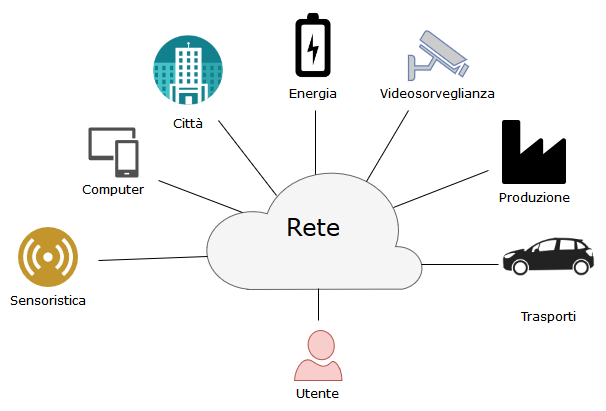
\includegraphics[width=0.9\columnwidth]{intro/iot}
    \caption{Rappresentazione figurata del concetto di \textit{"internet of things"}.}
    \label{fig:iot}
\end{figure}

Posso sintetizzare il concetto di \emph{Internet of Things} come quello di una rete di dispositivi interconnessi, individuabili in modo univoco e che possono comunicare informazioni.
I dispositivi presenti in una rete possono comunicare con due tipologie di attori diverse:
\setlist{nolistsep}
\begin{itemize}
  \item se la comunicazione avviene con altri dispositivi si parla di comunicazione M2M (\textit{Machine to Machine}, ovvero comunicazione tra macchine);
  \item se la comunicazione avviene interagendo con il mondo reale si parla di comunicazione M2H (\textit{Machine to Human}, ovvero comunicazione tra macchina e utente).
\end{itemize}

Il termine "Things" nel contesto IoT si riferisce a una varietà di dispositivi come ad esempio: videocamere di sorveglianza, automobili a guida autonoma e assistita oppure piccoli e grandi elettrodomestici casalinghi. Questi dispositivi, soprannominati anche \textit{smart object}, raccolgono informazioni utili in base agli attori con cui comunicano:
\setlist{nolistsep}
\begin{itemize}
  \item se i dispositivi comunicano in modo M2M, le informazioni supportano tecnologie esistenti, integrandosi nel flusso di informazioni esistente;
  \item se i dispositivi comunicano in modo M2H, le informazioni aiutano le persone che interagiscono con essi.
\end{itemize}

L'interesse verso il tema IoT è cresciuto esponenzialmente sia nel mercato consumer che in quello enterprise e secondo Forbes (\footcite{site:forbes-iot}) diventerà nel prossimo quinquennio uno dei settori dell'ITC più redditizi.
É interessante osservare anche la popolarità dei termini di ricerca correlati all'IoT: i dati sono stati ottenuti interrogando il servizio \url{https://trends.google.com/trends}, il quale consente di effettuare analisi sulla popolarità delle stringhe di ricerca immesse nel motore di ricerca di Google.
Ciascun grafico a linea (\textit{line chart} in inglese) presenta nelle ordinate il grado di popolarità della \textit{query} di ricerca, valutato da 0 (popolarità minima) a 100 (popolarità massima), e nelle ascisse l'arco temporale in analisi.

\begin{figure}[H]
    \centering
    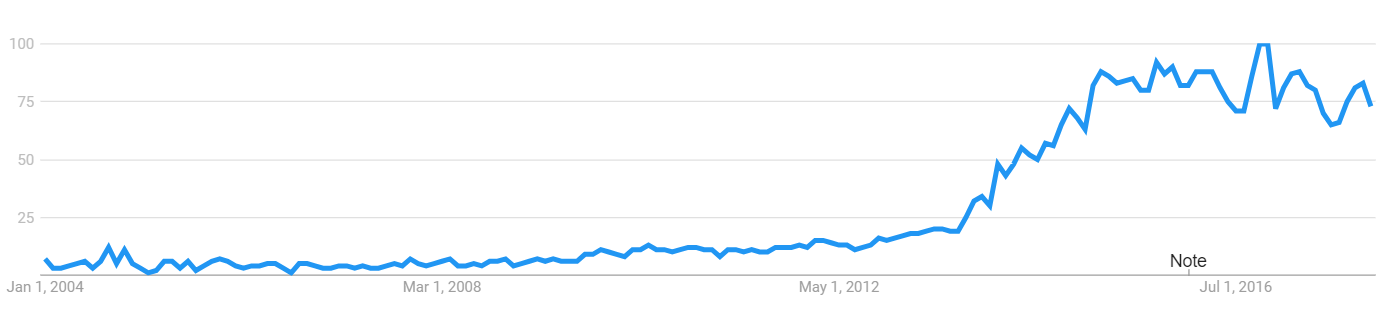
\includegraphics[width=0.9\columnwidth]{intro/internet-of-things-query-interest-worldwide}
    \caption{Andamento dell'interesse per la stringa di ricerca \textit{"internet of things"}. \\ \cite{site:iot-long-trend}}
    \label{fig:internet-of-things-query-interest}
\end{figure}

\begin{figure}[H]
    \centering
    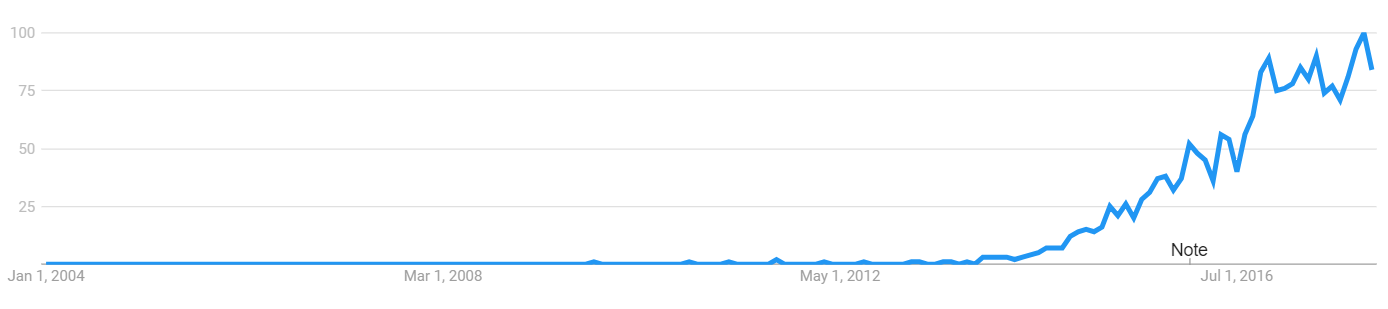
\includegraphics[width=0.9\columnwidth]{intro/iot-devices-query-interest-worldwide}
    \caption{Andamento dell'interesse per la stringa di ricerca \textit{"iot devices"}. \\ \cite{site:iot-devices-trend}}
    \label{fig:iot-devices-query-interest}
\end{figure}

\begin{figure}[H]
    \centering
    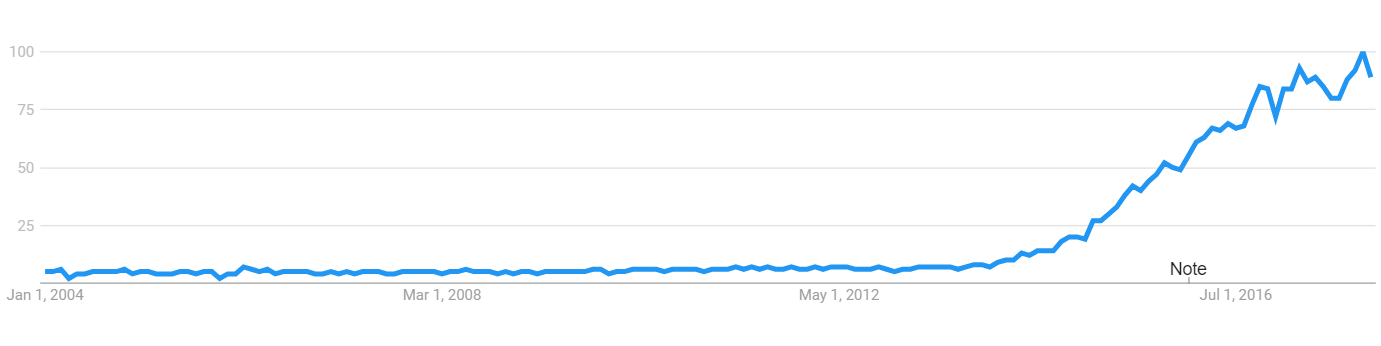
\includegraphics[width=0.9\columnwidth]{intro/iot-query-interest-worldwide}
    \caption{Andamento dell'interesse per la stringa di ricerca \textit{"iot"}. \\ \cite{site:iot-short-trend}}
    \label{fig:iot-query-interest}
\end{figure}

Sintetizzando le previsioni di Forbes con l'andamento dei termini di ricerca legati all'IoT, visibili alle figure ~\ref{fig:internet-of-things-query-interest}, ~\ref{fig:iot-devices-query-interest} e ~\ref{fig:iot-query-interest}, posso evidenziare che l'interesse verso l'argomento IoT stia generalmente aumentando o nel caso peggiore rimanga stabile con l'interesse degli anni precedenti.

\section{Architettura a microservizi: definizione e caratteristiche}
\label{intro:arch}

L'espressione \textbf{Architettura a microservizi} è sempre più comune tra gli sviluppatori di applicazioni \textit{enterprise} per descrivere un metodo di progettazione delle applicazioni come insiemi di servizi eseguibili indipendentemente, che comunicano tra loro grazie a meccanismi di comunicazione "leggeri" (solitamente attraverso \gls{api} HTTP).
Nella concezione originale in cui l'architettura a microservizi è nata, ogni servizio doveva essere progettato per eseguire in un processo indipendente dagli altri; con la nascita e la diffusione dei \emph{container} questo paradigma sta cambiando, associando sempre più l'esecuzione dei microservizi in altrettanti \emph{container}.
La \emph{containerization} (containerizzazione) è un metodo di virtualizzazione posto al livello del sistema operativo per la distribuzione ed esecuzione di applicazioni all'interno di \emph{container}.
\footcite{site:containerization}
Un \emph{container} è un unità \emph{software} standardizzata, distribuibile in un unico pacchetto composto da:
\setlist{nolistsep}
\begin{itemize}
  \itemsep0em
  \item l'applicazione da eseguire;
  \item l'ambiente d'esecuzione configurato correttamente per l'applicazione da eseguire, che a sua volta specifica:
  \begin{itemize}
    \item le dipendenze dell'applicazione;
    \item i file di configurazione dell'applicazione.
  \end{itemize}
\end{itemize}
Una delle tecnologie di containerizzazione che si è più diffusa è \href{https://www.docker.com/what-docker}{Docker} (\url{https://www.docker.com/what-docker}), sviluppata dall'omonima azienda; Docker ha reso disponibile la propria tecnologia di containerizzazione su molteplici piattaforme, sia locali (\emph{computer} con i sistemi operativi \emph{Windows}, \emph{macOS} e i sistemi operativi basati su \emph{Linux}) sia in \emph{cloud} (con ad es. servizi come \emph{Amazon Web Services} e \emph{Microsoft Azure}).
Per implementare il concetto di \emph{container}, la piattaforma di Docker installa un insieme di servizi che comunicano con il \gls{kernelg} del sistema operativo su cui è in esecuzione (\emph{host}) e con i quali gli utenti interagiscono per creare e gestire \emph{container}.
\footcite{site:docker-container}
Ho illustrato l'architettura sopra citata in figura ~\ref{fig:docker-arch}.

\begin{figure}[H]
    \centering
    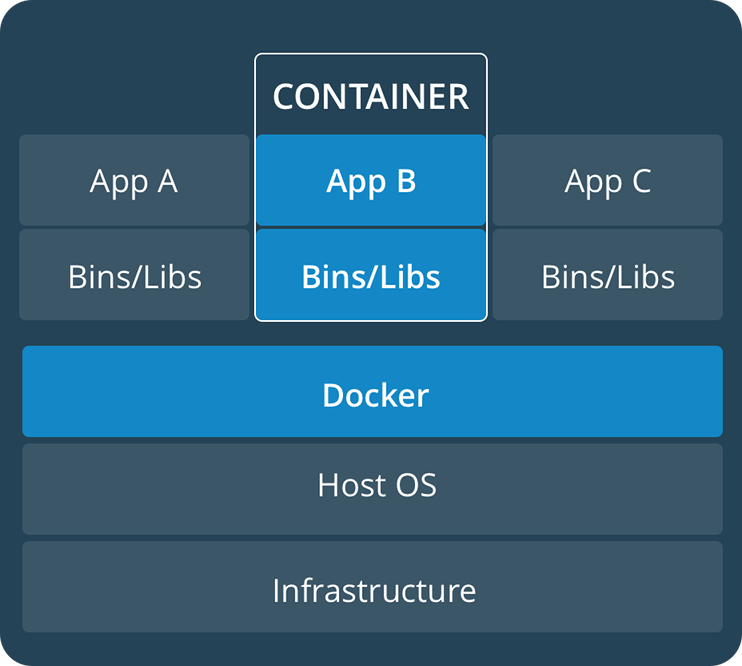
\includegraphics[scale=0.3]{intro/container}
    \caption{Architettura sviluppata da Docker per la sua piattaforma di containerizzazione.\\ \cite{site:docker-container}}
    \label{fig:docker-arch}
\end{figure}

\paragraph{Caratteristiche delle architetture monolitiche}

Un'applicazione monolitica è progettata e costruita per essere una singola unità in esecuzione.
L'applicazione sviluppata con architettura monolitica è responsabile della visualizzazione delle informazioni in un'interfaccia utente (pagine web o \emph{software} nativi), del reperimento delle informazioni da una sorgente di dati (solitamente un \emph{database}) e dell'esecuzione delle logiche di business della stessa.
\footcite{book:beginning-sw-eng}

Nelle applicazioni monolitiche la modularità del sistema si ottiene sfruttando i costrutti fondamentali dell'orientamento ad oggetti presente nei linguaggi di programmazione:
\setlist{nolistsep}
\begin{itemize}
  \item funzioni;
  \item classi;
  \item \emph{namespace} o \emph{package}.
\end{itemize}

\begin{figure}[H]
    \centering
    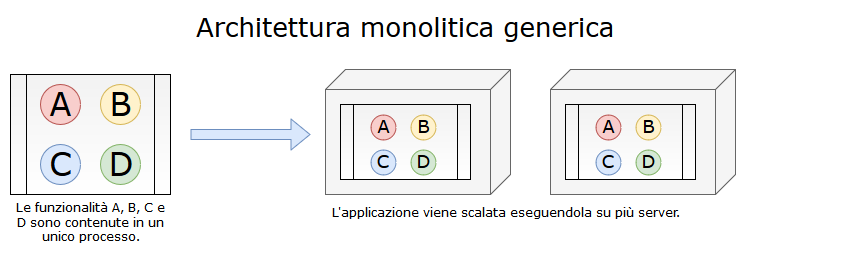
\includegraphics[scale=0.5]{intro/monolith-arch}
    \caption{Caratteristiche di una generica architettura monolitica.\\ \cite{site:fowler-microservices}}
    \label{fig:monolith-arch}
\end{figure}

Per aumentare la disponibilità delle applicazioni monolitiche si usa replicare istanze dell'applicazione in molteplici server, bilanciando il traffico verso le applicazioni per mezzo di un \gls{load balancerg}.
Tra i difetti delle applicazioni monolitiche posso evidenziare:
\setlist{nolistsep}
\begin{itemize}
  \item modifiche a una piccola parte all'applicazione richiedono la ricompilazione e la ridistribuzione dell'applicazione;
  \item all'accrescere della complessità dell'applicazione aumenta anche la difficoltà nel mantenere le modifiche isolate ai moduli di competenza;
  \item scalare l'applicazione richiede l'esecuzione di istanze multiple della stessa applicazione, ignorando di fatto eventuali requisiti di efficienza (solitamente alcune componenti del sistema non richiedono un aumento di \gls{throughputg}).
\end{itemize}

\paragraph{Caratteristiche delle architetture a microservizi}
\label{par:microservizi-intro}

Per lo stile architetturale a microservizi non esistono definizioni formali, tuttavia gli informatici più esperti in materia, tra i quali annovero Martin Fowler, hanno dedotto le caratteristiche che hanno accomunato i progetti diventati nel tempo esempi di best-practice.
Non tutte le architetture a microservizi hanno tutte le caratteristiche elencate in seguito, ma ci si aspetta che la maggior parte delle architetture esibisca quante più caratteristiche possibili.
\footcite{site:fowler-microservices}

L'aspetto cruciale delle architetture a microservizi verte sulla definizione di componente: la definizione comunemente accettata di componente è quella di "unità di software che è indipendentemente aggiornabile e sostituibile in un sistema".
Le architetture a microservizi usano i servizi per realizzare tale definizione di componente. A titolo di confronto con gli approcci di sviluppo tradizionali introduco la nozione di libreria.
Le librerie sono componenti insiti in un'applicazione tanto da risiedere nello stesso spazio di memoria dell'applicazione e che per essere invocate richiedono una chiamata di funzione in memoria.
I servizi sono componenti che vivono nel sistema come processi separati, sfruttando vari tipi di comunicazione interprocesso: richieste web, chiamate di funzione remote (RPC).
\footcite{site:fowler-microservices}

Il vantaggio principale dei servizi rispetto alle librerie consiste nel fatto che i servizi sono rilasciabili indipendentemente dal sistema.
Data la natura dell'architettura a microservizi, modifiche a un singolo servizio comportano il rilascio di una nuova versione solamente per quel servizio e non dell'intera applicazione.
Una buona architettura a microservizi quindi mira a progettare e implementare servizi che circoscrivano chiaramente il loro scopo.

\begin{figure}[H]
    \centering
    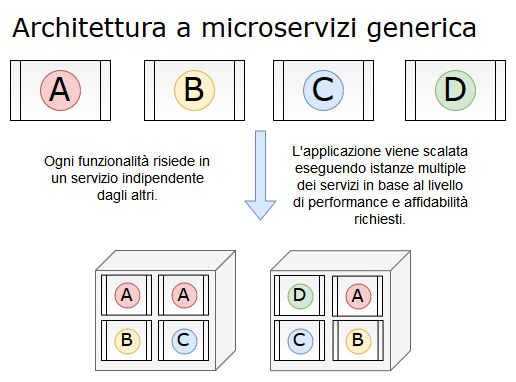
\includegraphics[scale=0.5]{intro/microservices-arch}
    \caption{Caratteristiche di una generica architettura a microservizi.\\ \cite{site:fowler-microservices}}
    \label{fig:microservices-arch}
\end{figure}

L'uso di servizi come componenti consente inoltre di rendere esplicita l'interfaccia dei componenti.
Spesso solamente la documentazione e la disciplina prevengono usi impropri di una componente da parte di uno sviluppatore esterno, rischiando di causare un alto accoppiamento tra componenti.
I servizi facilitano il rispetto delle interfacce pubblicate attraverso l'uso di meccanismi di chiamate remote esplicite.
Il difetto che Fowler attribuisce all'uso di servizi come componenti risiede nell'utilizzo di chiamate remote per la comunicazione tra servizi:
esse richiedono più risorse rispetto alle chiamate di funzione intraprocesso e quindi è necessario progettare le API di ciascun servizio rivolgendo maggiore attenzione all'aspetto prestazionale delle stesse.
\footcite{site:fowler-microservices}

Nella sua trattazione, Fowler inoltre riscontra ed evidenzia le differenze dal punto di vista della suddivisione delle persone impegnate nello sviluppo dell'applicazione.
Solitamente applicazioni complesse sviluppate seguendo l'architettura monolitica sono divise in \emph{team} con competenze isolate:

\setlist{nolistsep}
\begin{itemize}
  \item \emph{team} esperto in UI;
  \item \emph{team} specializzato in DB Management;
  \item uno o più \emph{team} specializzati a realizzare la logica di business.
\end{itemize}

Ho illustrato graficamente questo ambiente lavorativo in figura ~\ref{fig:business-organization}.
L'origine di una tale suddivisione risale alla Legge di Conway, enunciata nel 1967 dallo sviluppatore Melvin Conway, la quale afferma:
\begin{displayquote}
  "organizations which design systems ... are constrained to produce designs which are copies of the communication structures of these organizations."
\end{displayquote}

La legge di Conway ragiona sul fatto che un sistema \emph{software} complesso per funzionare richieda lo sforzo congiunto di più attori; dal momento che questi attori devono comunicare tra loro, la complessità insita nella comunicazione tra gli attori si riflette nelle componenti del sistema.
\footcite{site:conway}

\begin{figure}[H]
  \centering
  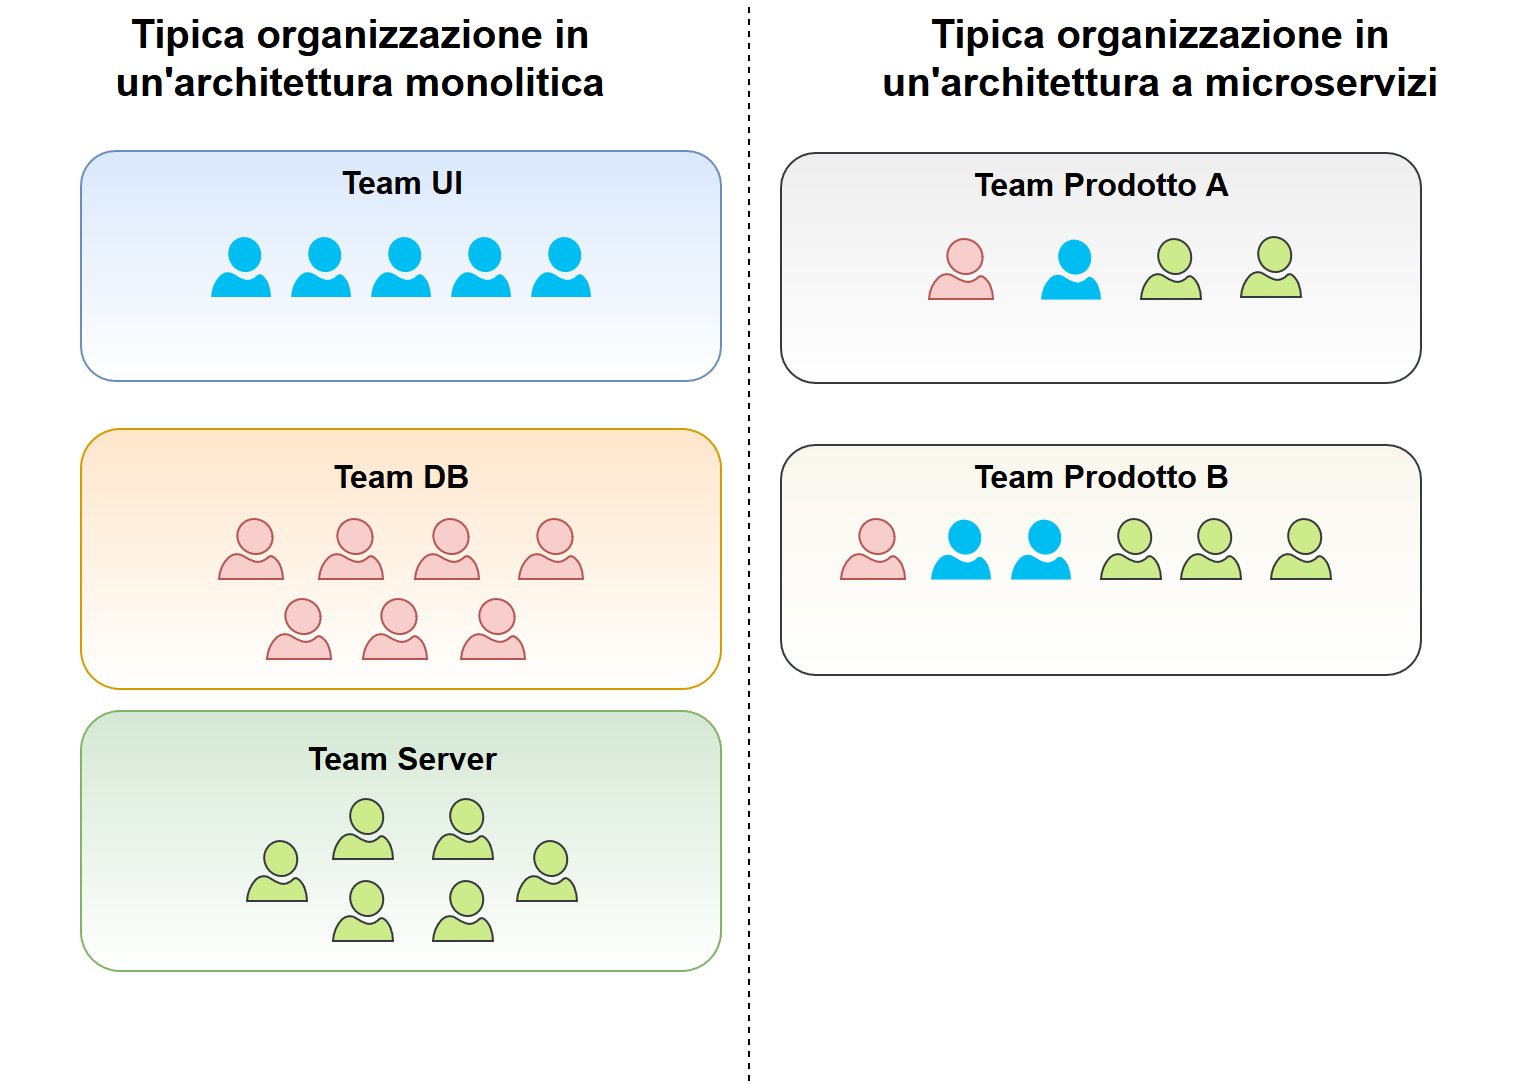
\includegraphics[width=0.9\columnwidth]{intro/business-organization}
  \caption{Illustrazione che mostra la differente organizzazione aziendale in un ambiente di sviluppo monolitico e in un ambiente di sviluppo a microservizi.\\ \cite{site:fowler-microservices}}
  \label{fig:business-organization}
\end{figure}

Quando le persone sono così isolate, anche una semplice modifica può richiedere l'intervento di altre persone in \emph{team} diversi.
La maggiore richiesta di pianificazione e organizzazione tra gruppi di sviluppo diversi causa un peggioramento dell'efficienza del processo di sviluppo.

L'approccio orientato ai microservizi con la suddivisione dell'applicazione invece pone l'accento sulle capacità di business: ogni \emph{team} inerente un particolare settore di business si occupa dell'intero prodotto per quel settore (sviluppando interamente UI, DB, ecc.).
I \emph{team} in questo approccio sono multidisciplinari e gli scambi con altri settori riflettono le effettive dipendenze tra un settore e un altro all'interno dell'azienda.
\footcite{site:fowler-microservices}

Un esempio di quest'approccio alla suddivisione lo si ritrova in Amazon, dove vige il motto "you build, you run it" ("tu lo costruisci, tu lo esegui").
In Amazon ogni \emph{team} ha completa responsabilità del prodotto anche in ambiente di produzione, mettendo in comunicazione diretta sviluppatori e utenti del prodotto per le attività di supporto e manutenzione.
\footcite{site:amazon-microservices}

Le comunicazioni tra servizi sono orchestrate usando semplici protocolli basati su REST.
REST, acronimo di REpresentational State Transfer, è un tipo di architettura \emph{software} per lo sviluppo di applicazioni distribuite, introdotta nel 2000 nella tesi di dottorato di Roy Fielding.
Le architetture basate su REST prevedono che la scalabilità delle applicazioni sia conseguenza di pochi principi di progettazione:

\setlist{nolistsep}
\begin{itemize}
  \item separazione tra \emph{client} e \emph{server}: i ruoli delle due componenti sono ben distinti utilizzando un insieme di interfacce comuni per la comunicazione, permettendo quindi uno sviluppo indipendente di queste componenti (se l'interfaccia comune non viene alterata);
  \item \emph{stateless}: la comunicazione \emph{client-server} è vincolata in modo che nessuna informazione sullo stato del \emph{client} venga memorizzata dal \emph{server};
  \item \emph{cacheable}: ogni \emph{client} deve poter memorizzare le risposte inviate dal \emph{server} per minimizzare le comunicazioni \emph{client-server}. Ogni risposta deve comunicare al \emph{client} implicitamente o esplicitamente se essa è memorizzabile;
  \item \emph{layered system}: un \emph{client} non deve poter discernere un \emph{server} di basso livello da uno intermedio, dedicato a migliorare le prestazioni o introdurre politiche di sicurezza;
  \item \emph{uniform interface}: la comunicazione tra \emph{client} e \emph{server} deve avvenire con un'interfaccia omogenea, disaccoppiando le due componenti ma degradando potenzialmente l'efficienza, dal momento che le informazioni vengono trasferite in una forma standardizzata invece di una più affine alla loro struttura.
\end{itemize}
\footcite{site:rest-wiki}
\footcite{rest-thesis}

L'esperienza di Fowler mostra come siano due le tipologie di protocolli più usati nelle architetture a microservizi:
\setlist{nolistsep}
\begin{itemize}
  \item protocolli basati su richieste/risposte HTTP secondo API ben dettagliate;
  \item protocolli basati sullo scambio di messaggi in un canale di comunicazione snello. I servizi producono e consumano i messaggi che circolano nel canale di comunicazione, secondo regole di accesso definite.
\end{itemize}

Quando un'applicazione è suddivisa in molteplici componenti sorgono naturalmente dubbi sulla gestione delle informazioni che ciascuna componente gestisce.
Solitamente nelle architetture monolitiche gli analisti astraggono i domini dell'applicazione scegliendo una fra le tecniche di modellazione disponibili e applicandola a tutti i domini;
i modelli prodotti sono poi veicolati su singoli \emph{storage} di dati (ad es. unico \emph{database}).
L'architettura a microservizi invece propone di concepire i modelli in autonomia per ogni singolo servizio, utilizzando le tecniche ritenute più appropriate.
Questa decentralizzazione dell'astrazione dei modelli si riflette anche sulla possibilità di decentralizzare le decisioni relative a quale \emph{storage} dei dati utilizzare per ciascun servizio.
Nell'architettura a microservizi si preferisce che ogni servizio gestisca il proprio \emph{database} in base ai requisiti che il servizio deve soddisfare: il database di un servizio potrebbe essere un'istanza di una stessa piattaforma tecnologica, una piattaforma specifica e ottimizzata per il caso d'uso del servizio oppure potrebbe non essere utilizzato (servizi puramente funzionali).
Questo approccio alla gestione della persistenza è chiamato \emph{Polyglot Persistence} ed è utilizzabile anche in architetture monolitiche, malgrado appaia con maggior frequenza in architetture a microservizi.
\footcite{site:fowler-microservices}

\begin{figure}[H]
    \centering
    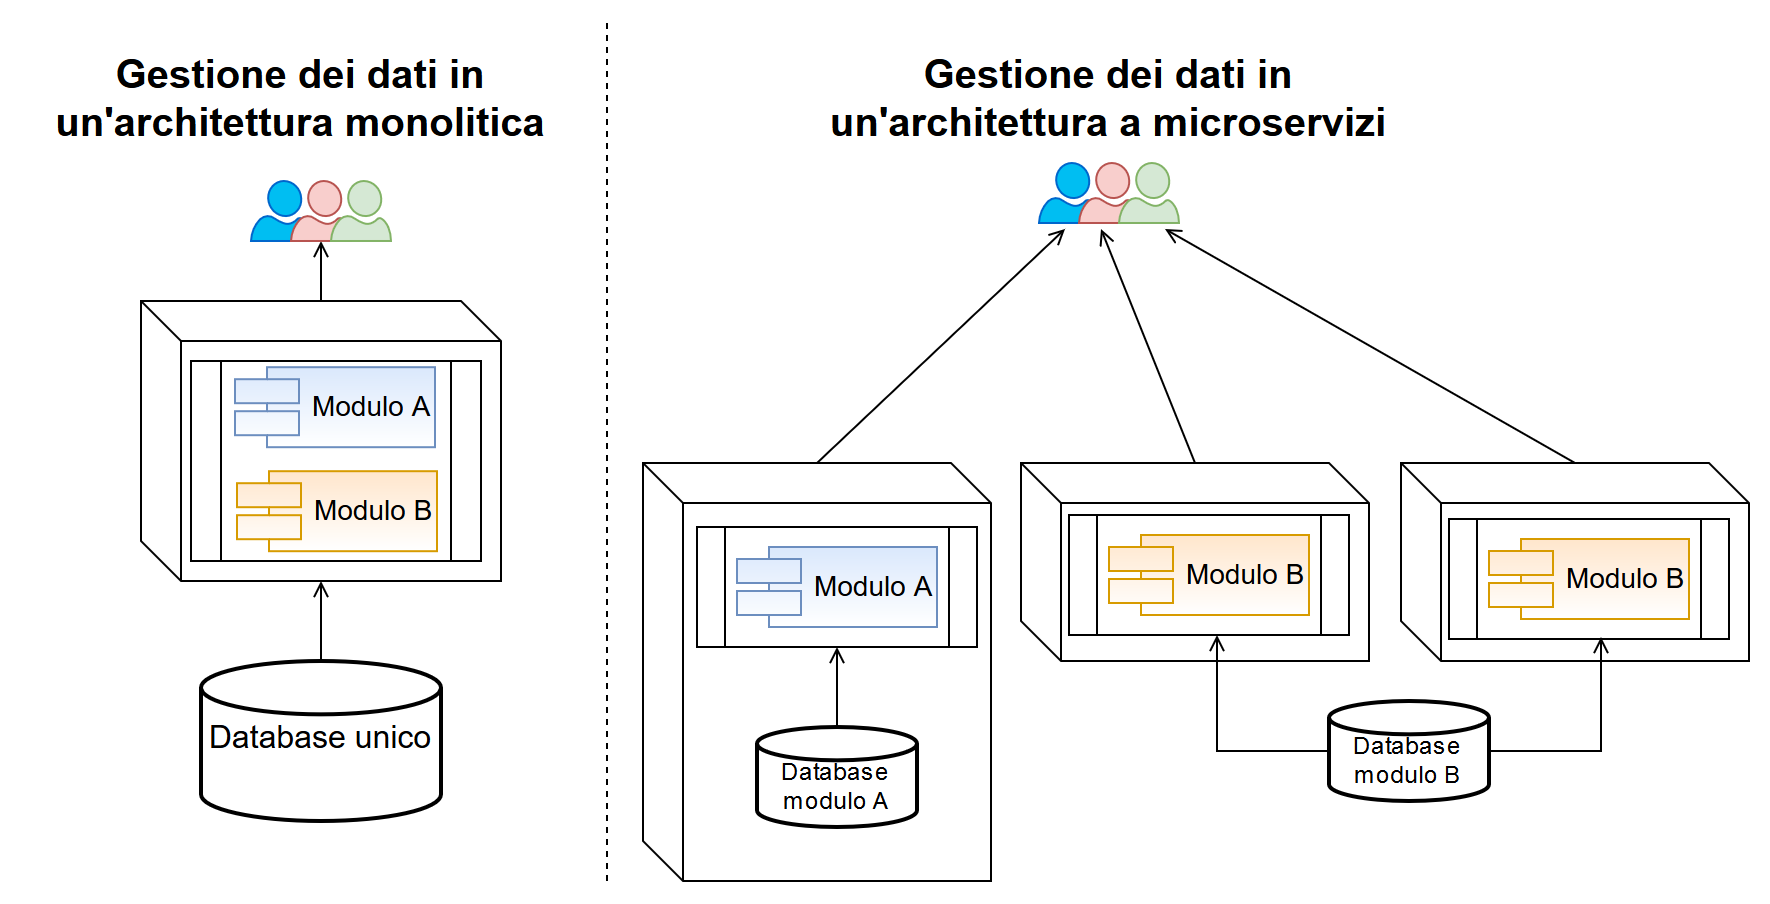
\includegraphics[width=0.9\columnwidth]{intro/data-storage}
    \caption{Illustrazione che mostra la differente gestione dell'architettura di persistenza dei dati tra prodotti software con architettura monolitica e con architettura a microservizi.\\ \cite{site:fowler-microservices}}
    \label{fig:data-storage}
\end{figure}

Le decisioni di \emph{storage} decentralizzate implicano una maggior attenzione verso gli aggiornamenti dei dati.
Fowler rileva che l'approccio comune agli aggiornamenti in un'architettura monolitica è quello di usare le transazioni per garantire la consistenza dei dati prima e dopo ciascun aggiornamento.
L'utilizzo di transazioni è un grave limite per l'architettura a microservizi, in quanto le transazioni impongono un ordine temporale che potrebbe non essere rispettato, causando inconsistenze dei dati salvati.
É per questo che le architetture a microservizi enfatizzano l'utilizzo di comunicazioni non vincolanti (\emph{transactionless}): eventuali inconsistenze vengono segnalate e risolte grazie a operazioni correttive.
\footcite{site:fowler-microservices}

Una conseguenza nell'utilizzo dei servizi come componenti è che le applicazioni devono prevedere e tollerare malfunzionamenti nei servizi. L'utilizzatore dei servizi deve quindi rispondere ai malfunzionamenti nel modo più elegante possibile.
É naturale quindi attribuire l'aumento di complessità della gestione dei malfunzionamenti tra i difetti delle architetture a microservizi.
Dal momento che i servizi possono malfungere in ogni momento, è fondamentale riuscire a:

\setlist{nolistsep}
\begin{itemize}
  \item monitorare il servizio,
  \item segnalare il malfunzionamento e
  \item ripristinare automaticamente il servizio
\end{itemize}
nel più breve tempo possibile. Conseguentemente, ogni servizio deve essere progettato focalizzando l'attenzione sulle attività di monitoring, individuando le metriche rilevanti (ad es. \emph{throughput}, latenza, ecc.).

Uno dei temi cruciali che ho riscontrato nella trattazione di Fowler consiste nel chiedersi quante responsabilità debba avere ciascun servizio: secondo Fowler la caratteristica fondamentale da osservare è la nozione di sostituzione e aggiornamento indipendenti.
Un buon segnale lo si ritrova quando ad ogni modifica di un servizio, questa modifica non richiede adattamenti in altri servizi (a meno di modifiche alle funzionalità offerte).
Se due o più servizi vengono aggiornati spesso insieme probabilmente essi dovrebbero essere uniti.
\footcite{site:fowler-microservices}

%**************************************************************
\pagebreak
\section{Valutazione dei rischi considerati nello stage}

\subsection{Valutazione dei rischi di uno stage interno}

Lo stage formativo viene previsto dal CdL triennale di Informatica in due modalità:
\setlist{nolistsep}
\begin{itemize}
  \item stage aziendali, riferiti anche come stage esterni, per i quali il proponente del progetto di stage è un'azienda;
  \item stage non aziendali, riferiti anche come stage interni individuali, per i quali il proponente del progetto di stage è un docente dell'Ateneo di Padova.
\end{itemize}


Sebbene lo stage aziendale sia la modalità preferita per svolgere l'attività, mi sono imbattuto in due ostacoli che mi hanno portato ad avviare uno stage interno. \\
Il mio stato di studente lavoratore causa il primo ostacolo: l'azienda per cui sono assunto non poteva offrire stage riguardanti il settore IoT.
Nel momento in cui ho iniziato a cercare proposte di stage e mi sono quindi informato sulle modalità con cui avrei potuto assentarmi da lavoro,
l'ufficio per le risorse umane dell'azienda per cui sono assunto mi ha comunicato che avrei avuto opzioni limitate, dipendenti dal motivo dell'assenza. \\
Se l'assenza avesse comportato l'inizio di attività lavorative per altre aziende (concorrenti oppure non concorrenti) sarei stato costretto a scegliere tra due opzioni:
\setlist{nolistsep}
\begin{itemize}
  \item il licenziamento dall'azienda per cui sono assunto;
  \item l'avvio della procedura di \gls{aspettativag} del lavoro come prevista dalla legge 53 recante data 8 marzo 2000. \footcite{site:aspettativa}.
\end{itemize}
Quindi fin dall'inizio la ricerca di un progetto di stage aziendale è stata fortemente messa in discussione dalle menzionate opzioni. \\
Malgrado il primo ostacolo, ho proseguito la ricerca dello stage aziendale al fine di ponderare se gli aspetti negativi legati al congedo lavorativo potessero essere in qualche modo bilanciati da eventuali esperienze formative.
\\
Dato il periodo di inizio dello stage (ottobre/novembre 2017), molti degli stage aziendali riguardanti il settore IoT proposti erano già stati svolti da altri studenti del corso.
Le poche proposte di stage aziendale legate al settore IoT rimanenti erano interessate alla integrazione con prodotti già esistenti:
malgrado l'opportunità offerta da queste aziende fosse interessante, ho riflettuto a lungo sul fatto che l'attività formativa non fosse adeguatamente supportata. \\
Nei progetti proposti infatti le aziende proponenti hanno enfatizzato l'utilizzo degli strumenti interni da loro sviluppati, da una parte per motivarmi ad essere assunto al termine dello stage,
dall'altra per effettivamente semplificarmi il lavoro nel processo di sviluppo. \\ \\
L'aspetto formativo è stato l'ambito più discusso per effettuare la scelta: malgrado la presenza di esperti nel settore mi interessasse,
per l'opportunità di approfondire l'ambito d'uso reale dei dispositivi \emph{smart}, la scelta di legarmi a un singolo prodotto, non particolarmente diffuso e utilizzato,
mi ha spinto ad iniziare a valutare il percorso di stage interno. \\

Ho riassunto i rischi considerati per lo svolgimento di uno stage interno individuale nella tabella ~\ref{tab:rischi-stage-interno}.

\begin{table}
\caption{Tabella di analisi dei rischi correlati allo svolgimento di uno stage interno}
\label{tab:rischi-stage-interno}
\begin{tabularx}{\linewidth}{|p{7.5cm}|X|X|}
\hline
\textbf{Rischio} & \textbf{Probabilità di accadimento} & \textbf{Gravità del danno potenziale}\\
\hline
Il lavoro svolto individualmente, senza possibilità di essere guidato da esperti nel settore, potrebbe risultare ininfluente. La presenza di una persona con più esperienza in un determinato tema è utile in quanto può focalizzare l'attenzione su problematiche reali, le quali potrebbero non essere correttamente valutate nel momento in cui si dispone di scarsa esperienza in materia. & Molto probabile & Grave \\
\hline
Il lavoro svolto individualmente, senza possibilità di essere guidato da esperti nel settore, potrebbe procedere più lentamente, causando il non raggiungimento degli obiettivi preposti. & Molto probabile & Media \\
\hline
\end{tabularx}
\end{table}


\subsection{Valutazione dei rischi del tema IoT}

Nuove tecnologie contengono sempre una determinata quantità di rischi: mentre la maggior parte degli sviluppatori trovano utilizzi per i dispositivi IoT,
altri cercano modi per usarli per scopi meno nobili. \\
I dispositivi IoT stanno sempre più diffondendosi in molti aspetti su cui basiamo la società moderna:
\setlist{nolistsep}
\begin{itemize}
  \item trasporti;
  \item comunicazione;
  \item settore energetico.
\end{itemize}

Attacchi informatici contro questi dispositivi possono portare al caos: dalla distruzione di proprietà alla messa in discussione della propria sicurezza, con l'accezione che il termine \emph{safety} possiede nella lingua inglese.
A peggiorare la situazione, gli acquirenti di questi dispositivi pretendono che essi continuino a funzionare per una quantità di tempo superiore a quella che il consumismo tecnologico ha abituato. \\
La quantità di protocolli sviluppati per l'IoT porta ad aumentare la complessità insita in questi dispositivi.
Una complessità maggiore implica un maggior costo per le società per aggiornare i prodotti rilasciati, portando quindi i produttori ad abbandonare i dispositivi rilasciati da più tempo, ignorando l'insorgere di nuove vulnerabilità.

Date le suddette premesse, per il settore IoT ho posto numerose osservazioni relative ai rischi collegati allo sviluppo di prodotti software e hardware. I rischi considerati sono riassunti nella tabella ~\ref{tab:rischi-iot}.
\begin{table}[H]
\caption{Tabella di analisi dei rischi correlati al tema IoT}
\label{tab:rischi-iot}
\begin{tabularx}{\linewidth}{|p{7.5cm}|X|X|}
\hline
\textbf{Rischio} & \textbf{Probabilità di accadimento} & \textbf{Gravità del danno potenziale}\\
\hline
Lo sviluppo di prodotti legati all'IoT espone l'utente degli stessi a possibili rischi di cybersicurezza: il furto di dati ma soprattutto la perdita di controllo dell'utente sui propri dispositivi sono scenari possibili e con conseguenze disastrose per lo sviluppatore di tale prodotto. & Probabile & Molto grave \\
\hline
La mole di dati raccolta dai dispositivi inseriti in un contesto IoT potrebbe essere tale da richiedere investimenti consistenti per la loro elaborazione e per mantenere elevata la loro confidenzialità. Inoltre la diversità dei dispositivi presenti in una rete aumenta la complessità del trattamento delle informazioni. & Probabile & Media \\
\hline
Dal momento che l'IoT è un ambito emergente nel contesto ITC ho osservato la nascita di una multitudine di protocolli per la raccolta e la trasmissione delle informazioni, nessuno dei quali è stato indicato o si è imposto come standard globale. & Molto probabile & Media \\
\hline
\end{tabularx}
\end{table}


\subsection{Valutazione dei rischi dell'architettura a microservizi}

L'architettura a microservizi permette di sviluppare un'applicazione complessa partendo da piccole e relativamente isolate componenti;
in questo modo i cambiamenti effettuati sono facilmente verificabili.
La frammentazione dell'architettura del prodotto rende tuttavia più complesse le attività di test funzionali, perché per eseguire un tipico caso d'uso di una funzionalità completa sono richiesti molteplici servizi, correttamente configurati per comunicare tra loro ed eseguire simultaneamente. \\ \\
Lo sviluppo di servizi indipendenti rende inoltre difficoltosa l'attività di integrazione delle modifiche: nel momento in cui molti \emph{team} di sviluppo lavorano ciascuno nel proprio servizio non è possibile integrare queste modifiche senza una attenta pianificazione, che coinvolga la comunicazione dei cambiamenti effettuati. \\
Nel mio caso questo non si applica, lavorando individualmente, tuttavia mi sono comunque richieste le attività di allineamento delle funzionalità tra i servizi che necessitano di comunicare tra loro. \\ \\
Anche in questo caso, la relativa novità dell'argomento causa una generale mancanza di documentazione pratica, lasciando lo spazio ad esempi semplici, che non riflettono applicazioni d'uso reale, oppure documentazione teorica, che non si spinge ad analizzare problematiche reali.
La tabella ~\ref{tab:rischi-arch-microservizi} riassume e sintetizza i rischi analizzati in precedenza.

\begin{table}[H]
\caption{Tabella di analisi dei rischi correlati all'utilizzo dell'architettura a microservizi}
\label{tab:rischi-arch-microservizi}
\begin{tabularx}{\linewidth}{|p{7.5cm}|X|X|}
\hline
\textbf{Rischio} & \textbf{Probabilità di accadimento} & \textbf{Gravità del danno potenziale}\\
\hline
Spostamento di alcune problematiche di progettazione da un livello di modulo a un livello di architettura del sistema. & Probabile & Media \\
\hline
Le performance dell'applicazione sviluppata potrebbero non essere sufficienti passando da un'architettura monolitica a una a microservizi. & Scarsamente probabile & Grave \\
\hline
Difficoltà nel reperimento delle informazioni, data la relativa novità dell'argomento. Assume maggior significato nel momento in cui l'esperienza con un tale paradigma risulti scarsa o nulla. & Molto probabile & Grave \\
\hline
\end{tabularx}
\end{table}

\section{Organizzazione dello stage}

Ho pianificato le attività, in termini di quantità di ore di lavoro, secondo la tabella ~\ref{tab:organizzazione-stage} e le ho inserite in un Piano di Lavoro.
Dal momento che ho già avuto modo di trattare il lato tecnologico del progetto nel corso del percorso di studi, ho allocato 40 ore di formazione negli argomenti meno conosciuti e li ho suddivisi in due parti:
\begin{itemize}
  \item una prima parte in cui ho studiato le caratteristiche comuni delle architetture a microservizi e i Design Pattern nati per facilitare l'implementazione di un sistema con questo tipo di architettura;
  \item una seconda parte pratica di applicazione dei princìpi teorici in Node.js e il ripasso della caratteristiche tecniche del \emph{framework} React.
\end{itemize}
Durante quest'insieme di attività di formazione, per mitigare i rischi elencati in tabella ~\ref{tab:rischi-stage-interno}, ho focalizzato la mia attività di studio alla ricerca di esempi sviluppati da aziende con esperienza in materia per risolvere i problemi che hanno dovuto affrontare.
Il secondo macroblocco di attività riguarda l'analisi, la progettazione e l'implementazione dei servizi di comunicazione con i dispositivi. A queste attività ho allocato 120 ore, in quanto per mitigare le probabilità di incorrere nei rischi elencati in tabella ~\ref{tab:rischi-iot} ho assegnato risorse per l'attività di ricerca del protocollo di comunicazione da implementare. Durante le attività di analisi inoltre mi sono preparato per contrastare i rischi più probabili che ho menzionato in tabella ~\ref{tab:rischi-arch-microservizi}, analizzando i requisiti funzionali del sistema e mettendoli in relazione con le attività di ricerca effettuate durante le attività di formazione. Ho incluso nelle attività di progettazione di questo blocco anche la progettazione e realizzazione dei dispositivi "virtualizzati", l'implementazione dei quali mi ha permesso di effettuare i primi test dei servizi di comunicazione.
Il terzo macroblocco di attività riguarda l'analisi dell'interazione che un \emph{client} può avere con i servizi di comunicazione, permettendomi di arrivare alla progettazione e realizzazione del servizio che compone le funzionalità da offrire alla \emph{dashboard} e la \emph{dashboard} stessa.
L'ultimo blocco di attività riguarda la revisione del prototipo implementato e la sua possibile pubblicazione sulla piattaforma di Heroku\footcite{heroku}.

\begin{table}[H]
	\caption{Tabella che illustra la pianificazione delle attività dello stage}
	\label{tab:organizzazione-stage}
	\begin{tabular}{|>{\centering} m{1.5cm}|>{\centering} m{1.5cm}|m{10cm}|}
		\hline
		\multicolumn{2}{|c|}{\textbf{Durata in ore}} & \textbf{Descrizione dell'attività} \\
		\hline
		\multicolumn{2}{|c|}{40} & Formazione
	 	\begin{itemize}
			\item Architettura microservizi
			\item Node.JS orientato ai microservizi
			\item React
		\end{itemize}
		\\
		\hline
		\multirow{4}{*}{120} & & Analisi, sviluppo e implementazione servizi di comunicazione con i dispositivi IoT\\
		\cline{2-2}
		& 40 & \begin{itemize}
			\item Analisi dei protocolli \emph{open source} esistenti per i diversi dispositivi IoT
			\item Stima implementazione eventuali nuovi protocolli
			\end{itemize} \\
			\cline{2-2}
			& 80 & \begin{itemize}
			\item Progettazione dei servizi di comunicazione con i dispositivi
			\item Progettazione dei test dei servizi di comunicazione
			\item Realizzazione dei test e dei servizi di comunicazione in Node.js
		\end{itemize} \\
		\hline
		\multirow{4}{*}{120} & & Analisi, sviluppo e implementazione servizio di presentazione delle informazioni agli utenti\\
		\cline{2-2}
		& 40 & \begin{itemize}
		\item Analisi interazione utente con la \textit{dashboard}
		\end{itemize} \\
		\cline{2-2}
		& 80 & \begin{itemize}
			\item Progettazione del servizio di presentazione informazioni
			\item Progettazione dei test del servizio di presentazione
			\item Realizzazione dei test e del servizio di presentazione in React, HTML5 e CSS3.
		\end{itemize} \\
		\hline
		\multicolumn{2}{|c|}{20} & {\textit{Review} dei servizi, \textit{deploy} dei servizi su Heroku.}\\
		\hline
		\multicolumn{2}{|c|}{\textbf{Totale ore}} & {\textbf{300}} \\
		\hline
\end{tabular}
\end{table}
% Le settimane sono composte da 40 ore totali di impegno sul progetto,

\section{\emph{Milestone}}
In questa sezione presento le \gls{milestone} previste per il progetto su base settimanale, associando a ciascuna \emph{milestone} i prodotti che devono essere sviluppati entro la corrispondente scadenza.
\begin{itemize}
	\item Prima settimana: Completamento delle attività di autoformazione con produzione di una breve relazione riguardante la stessa;
	\item Seconda e terza settimana: Analisi dei protocolli di comunicazione esistenti, primo ciclo di progettazione e implementazione del servizio di comunicazione, mirato all'implementazione dei dispositivi \textit{virtualizzati};
	\item Quarta e quinta settimana: Revisione analisi sui protocolli, secondo ciclo di progettazione e implementazione del servizio di comunicazione, mirato all'implementazione dei dispositivi fisici (Raspberry Pi);
	\item Sesta e settima settimana: Analisi dell'interazione utente con la \emph{dashboard}, progettazione e implementazione del servizio di presentazione;
	\item Ottava settimana: Revisione dei servizi, stesura del Manuale d'Uso e deploy (opzionale) di un ambiente di simulazione della \emph{dashboard} su Heroku.
\end{itemize}
             % Introduzione
% !TEX encoding = UTF-8
% !TEX TS-program = pdflatex
% !TEX root = ../relazione-finale.tex

%**************************************************************
\chapter{Progetto di Stage}
\label{cap:processi-metodologie}
%**************************************************************

\intro{Nelle sezioni di questo capitolo parlerò delle aspettative e degli obiettivi posti inizialmente per il progetto di Stage}\\

%**************************************************************
\section{Obiettivi curricolari}

Questa sezione risponde alla domanda:

Quali valori mi \textbf{aspetto} di dedurre dall'esperienza di stage che siano rilevanti sul mercato del lavoro?

Parlerò della rilevanza del mercato IoT, in continua espansione.

Parlerò inoltre del crescente interesse delle aziende verso il paradigma dell'architettura a microservizi.


%**************************************************************
\section{Obiettivi formativi}

Questa sezione risponde alla domanda:

Quali informazioni mi \textbf{aspetto} di imparare/studiare durante lo svolgimento dello Stage?

Parlerò dei concetti imparati per supportare al meglio lo sviluppo di applicazioni con architettura a microservizi.
I concetti principali sono: polyglot persistence, gateway pattern, analisi della corretta dimensione di un servizio per essere definito un microservizio.
Per quanto riguarda l'IoT parlerei dei protocolli analizzati durante l'attività di formazione, soffermandomi in particolare su MQTT.


%**************************************************************
\section{Obiettivi tecnici}

Questa sezione risponde alle domande:

Quali tecnologie mi \textbf{aspetto} di imparare a padroneggiare durante lo svolgimento dello Stage?
Quali competenze mi \textbf{aspetto} di apprendere durante lo svolgimento dello Stage?

Per quanto riguarda l'architettura a microservizi, mi aspetto di padroneggiare l'utilizzo del gateway pattern e di cominciare a costruire esperienza sulla composizione di servizi e sul loro dimensionamento.
Per quanto riguarda l'IoT mi aspetto di aver appreso MQTT nel suo utilizzo come protocollo molti-a-molti, uno-a-molti e uno-a-uno.

%**************************************************************
\section{Obiettivi di prodotto}

Questa sezione risponde alla domanda:

Quali caratteristiche (innovative o non) del prodotto sviluppato mi \textbf{aspetto} di poter dimostrare?

L'aspetto innovativo del prodotto che mi aspetto di evidenziare è quello della scalabilità del prodotto e la possibilità di gestire dispositivi che dichiarino azioni.
             % Processi
% !TEX encoding = UTF-8
% !TEX TS-program = pdflatex
% !TEX root = ../relazione-finale.tex

%**************************************************************
\pagebreak
\chapter{Svolgimento dello stage}
\label{cap:descrizione-stage}
%**************************************************************

\section{Ambiente di sviluppo}

In questa sezione descrivo le tecnologie e gli strumenti di sviluppo che ho utilizzato per lo sviluppo del progetto, includendo la motivazione per cui ho fatto la scelta.
Nella tabella ~\ref{tab:tecnologie} presento il sommario delle tecnologie e degli strumenti che ho utilizzato per lo sviluppo del prototipo, indicandone:
\begin{itemize}
  \item il nome;
  \item una breve descrizione;
  \item la versione utilizzata o l'intervallo di versioni utilizzate nel caso in cui abbia aggiornato le tecnologie o gli strumenti utilizzati ad una versione successiva;
  \item il grado di conoscenza pregressa in una scala crescente che parte da 0 (esperienza nulla) e che arriva a 5 (esperienza consolidata), abbreviato in "Esp.".
\end{itemize}

\begin{table}[!htbp]
\caption{Tabella con il sommario delle tecnologie e degli strumenti utilizzati}
\label{tab:tecnologie}
\begin{tabularx}{\linewidth}{|c|>{\hsize=1.6\hsize}X|>{\hsize=0.4\hsize}X|c|}
\hline
\textbf{Tecnologia} & \textbf{Descrizione} & \textbf{Versioni} & \textbf{Esp.}\\
\hline
Node.js & Node.js è un ambiente d'esecuzione utilizzato per l'implementazione di applicazioni server in JavaScript. & v9.2.0, \newline v9.2.1 & 4 \\
\hline
React & React è una libreria per il linguaggio JavaScript il cui scopo è costruire interfacce grafiche. & v16.2.0 & 3 \\
\hline
ECMAScript 2017 & ECMAScript è un linguaggio di programmazione la cui implementazione standard più conosciuta è JavaScript. & 06/2017 & 2 \\
\hline
Jest & Jest è un \emph{framework} per l'implementazione di test per codice JavaScript. & v21.2.1 & 3 \\
\hline
ESLint & ESLint è uno strumento \emph{open source} per l'analisi statica del codice JavaScript prodotto. & v4.12.0, \newline v4.12.1 & 4 \\
\hline
HTML5 & HTML5 è un linguaggio di \emph{markup} per la formattazione e impaginazione delle pagine \emph{web}. & N.D. & 4 \\
\hline
CSS3 & CSS3 è un linguaggio di formattazione delle pagine \emph{web}. & N.D. & 2 \\
\hline
Docker Engine & Docker Engine è la combinazione dell'implementazione della tecnologia di containerizzazione con gli strumenti di gestione del ciclo di vita dei \emph{container}. & v17.09.0, \newline v17.12.0 & 4 \\
\hline
Docker Compose & Docker Compose è lo strumento attraverso cui è possibile coordinare applicazioni eseguite su \emph{container} multipli. & v1.18.0 & 1 \\
\hline
Atom & Atom è un \emph{editor} di testo sviluppato da \gls{GitHub}. & v1.21.2, \newline v1.23.1 & 4 \\
\hline
VS Code & Visual Studio Code è un \emph{editor} di testo sviluppato da \gls{Microsoft}. & v1.18.1, \newline v1.19.1 & 1 \\
\hline
\end{tabularx}
\end{table}

% \subsection{Node.js}
%



% \section{MQTT}
% \label{subsec:mqtt}
%
%
% MQTT mira ad assere una soluzione semplice da implementare, per permettere la maggior copertura di dispositivi possibile.
% MQTT usa messaggistica pub/sub per permettere ai dispositivi di pubblicare nella rete informazioni non predefinite.
% MQTT non richiede amministrazione in quanto cerca di rispondere ad eventi inaspettati in maniera semplice e con maggior buon senso possibile.
% MQTT minimizza il traffico sulla rete introducendo un \gls{overhead} sui dati minimo.
% MQTT si aspetta di lavorare in reti con frequenti interruzioni, utilizzando il meccanismo dell'ultimo testamento.
% MQTT si accorge repentinamente di cambiamenti dello stato della sessione.
% MQTT si aspetta che i \emph{client} abbiano risorse d'elaborazione limitate.
% MQTT mette a disposizione livelli di affidabilità per la trasmissione di informazioni critiche.
% MQTT non fa assunzioni sulla struttura né il contenuto dei dati.

\newpage

%**************************************************************
\section{Analisi dei requisiti}
\label{ar}

Ho iniziato l'Analisi dei requisiti cercando di capire quali funzionalità dovesse offrire il prototipo; per affrontare al meglio la definizione di queste funzionalità, ho esplorato il mercato dei dispositivi IoT esistenti per individuare i limiti del dominio applicativo in cui questi dispositivi si inseriscono.
Ho osservato che una delle caratteristiche desiderabili che il sistema deve offrire riguarda l'identificazione precisa di quali dispositivi sono collegati al sistema; per questo ho vincolato l'accesso dei dispositivi al sistema: per accedervi i dispositivi devono fornire informazioni relative a modello, revisione, produttore e anno di produzione del dispositivo, oltre a un seriale univoco.

Ho inoltre suddiviso i dispositivi in due tipi principali in base alle funzionalità che essi offrono:
\begin{itemize}
	\item sensori;
	\item dispositivi che ho definito "attivi".
\end{itemize}
La funzionalità principale offerta dai sensori è l'invio periodico di informazioni legate a ciò che il sensore misura.
L'invio di informazioni periodiche avviene in automatico, secondo i parametri impostati dal produttore del sensore.

Nella mia analisi delle funzionalità richieste dai dispositivi attivi, ho considerato le seguenti funzionalità:
\begin{itemize}
	\item pubblicazione di una lista degli eventi gestiti dal dispositivo;
	\item generazione di risposte agli eventi esterni;
	\item invio di informazioni sullo stato energetico del dispositivo;
	\item spegnimento del dispositivo.
\end{itemize}

Il dispositivo espone la lista degli eventi gestiti; questa lista permette di conoscere le funzionalità \emph{smart} del dispositivo.
La funzionalità di risposta agli eventi gestiti è automatica, avviene a ogni evento occorso ed è gestita direttamente dal produttore del dispositivo.
L'invio delle informazioni sullo stato energetico del dispositivo richiede che il produttore abbia dotato il dispositivo di unità di \emph{power management} e perciò potrebbe non essere disponibile per tutti i dispositivi collegati.

Acquisita conoscenza del dominio applicativo in cui mi stavo muovendo, ho introdotto il concetto di "centro di controllo": nella mia analisi, il centro di controllo consiste in quell'insieme di dispositivi responsabili della coordinazione tra i vari dispositivi connessi alla rete.
I dispositivi facenti parte del "centro di controllo" presentano le seguenti funzionalità:
\begin{itemize}
	\item gestione dei dispositivi collegati al sistema;
	\item ricezione, elaborazione e memorizzazione delle informazioni utili provenienti dai dispositivi (anche per fini diagnostici);
	\item pubblicazione delle informazioni raccolte per i \emph{client} che interrogano il centro di controllo.
\end{itemize}
Dal momento che i dati ricevuti dal centro di controllo potrebbero essere raccolti dai dispositivi in una forma grezza, ho concluso che il centro di controllo necessiti di capacità di elaborazione al fine di rendere i dati raccolti comprensibili anche agli umani.

Individuate le necessità dei dispositivi coinvolti, ho iniziato lo studio dei protocolli di comunicazione. \gls{MQTT} è un protocollo di messaggistica leggero basato sul \emph{Design Pattern} \emph{Publish/Subscribe}.
É un protocollo nato per l'utilizzo con sensori a basso consumo energetico ed è stato progettato tra la fine degli anni '90 e l'inizio degli anni 2000 per ambienti in cui l'affidabilità della rete non era garantita.\footcite{mqtt}
I dispositivi che ho considerato comunicano con il sistema utilizzando il protocollo MQTT (~\ref{subsec:mqtt}), perché ho ritenuto questo protocollo il più adatto per il sistema.
I motivi che mi hanno spinto a scegliere MQTT sono elencati di seguito:
\begin{itemize}
	\item è un protocollo molto diffuso, caratteristica che mi ha facilitato molto nella ricerca di documentazione che dimostri il suo utilizzo;
	\item è un protocollo \emph{data agnostic}, ossia che non pone vincoli sulla struttura dei dati scambiati nella rete;
	\item è un protocollo efficiente in quanto trasmette informazioni con un \emph{overhead} minimo;
	\item è un protocollo che permette l'aggiunta e la rimozione di dispositivi dinamicamente, richiedendo intervento manuale minimo all'utente.
\end{itemize}

Nella mia analisi dell'interazione dell'utente con la \emph{dashboard} ho specificato che l'accesso alle funzionalità del prodotto avvenga attraverso una interfaccia \emph{web}, opportunamente progettata per essere reattiva (ottimizzata per \emph{mobile}). Ho considerato anche la realizzazione di applicazioni native per i dispositivi \emph{mobile}, tuttavia per la realizzazione del prototipo ho preferito concentrare le mie attività nell'implementazione di una soluzione multi-piattaforma.
Durante le attività di analisi dei requisiti ho scritto un documento di Analisi dei Requisiti, nel quale ho indicato gli obiettivi e le funzionalità del prototipo e dei dispositivi.
Per raccogliere e specificare i requisiti del sistema e integrarli nel documento di Analisi dei Requisiti ho utilizzato i seguenti strumenti:
\begin{itemize}
  \item casi d'uso, che permettono di valutare ogni requisito sulla base degli attori che interagiscono con il sistema, rispettando le aspettative che l'attore tiene dall'avvio dell'interazione al termine della stessa;
  \item diagrammi \gls{uml} dei casi d'uso, che permettono di rappresentare i casi d'uso attraverso una definizione delle relazioni tra sistema, attori e funzionalità che il sistema offre agli attori.
\end{itemize}
Nella stesura dell'Analisi dei Requisiti ho utilizzato \emph{template} per velocizzare la definizione dei casi d'uso e dei requisiti.
Nei \emph{template} che ho utilizzato, ho catalogato i casi d'uso nella forma seguente:

\begin{figure}[H]
  \centering
  \[ UC[numero][caso] \]
  \begin{tabular}{@{}>{$}l<{$}l@{}}
    UC & specifica che si sta parlando di un caso d’uso;\\
    numero & è assoluto e rappresenta un riferimento univoco al caso d’uso in questione;\\
    caso & individua eventuali diramazioni all'interno dello stesso caso d’uso.\\
  \end{tabular}
\end{figure}

La breve descrizione di ciascun caso d’uso presenta:
\begin{itemize}
	\item gli attori del caso d’uso;
	\item lo scopo e la descrizione del caso d’uso.
\end{itemize}

Gli attori che ho considerato in sede di analisi consistono in:
\begin{itemize}
	\item Utente: rappresenta l'utente che interagisce con la \emph{dashboard};
	\item Dispositivi: rappresentano l'insieme di apparati collegati al sistema che forniscono i dati per popolare la \emph{dashboard};
	\item Dispositivo: rappresenta uno dei dispositivi collegati al sistema;
	\item Interfaccia proprietaria del dispositivo: rappresenta l'interfaccia proprietaria progettata dal produttore di un generico dispositivo.
\end{itemize}

% ![Sommario dei casi d'uso](./images/use_cases.png)
% <p align="center"><i>Sommario dei casi d'uso</i></p>

Lo scenario principale che ho immaginato, descritto nel caso d'uso ~\ref{uc:scenario-principale} e illustrato utilizzando il linguaggio UML in figura ~\ref{fig:scenario-principale}, prevede che l'utente abbia correttamente installato il prototipo per effettuare le prove in una macchina in locale e abbia eseguito l'accesso alla \emph{dashboard}. A questo punto ho previsto che l'utente possa utilizzare tre funzionalità della \emph{dashboard}:
\begin{itemize}
  \item visualizzare una pagina con il riepilogo dei dispositivi collegati;
  \item visualizzare una pagina che permetta di gestire i dispositivi collegati;
  \item visualizzare una pagina che indichi lo stato del sistema.
\end{itemize}

% uc testuale
\begin{usecase}{0}{Scenario principale}
\usecaseactors{Utente, Dispositivi}
\usecasepre{L'utente ha correttamente installato il prototipo e ha aperto la \emph{dashboard} in un \emph{browser}}
\usecasedesc{La \emph{dashboard} mostra lo stato del sistema ed evidenzia i dispositivi collegati}
\usecasepost{La \emph{dashboard} consente un'altra interazione con il sistema}
\label{uc:scenario-principale}
\end{usecase}

% uc figura
\begin{figure}[!h]
    \centering
    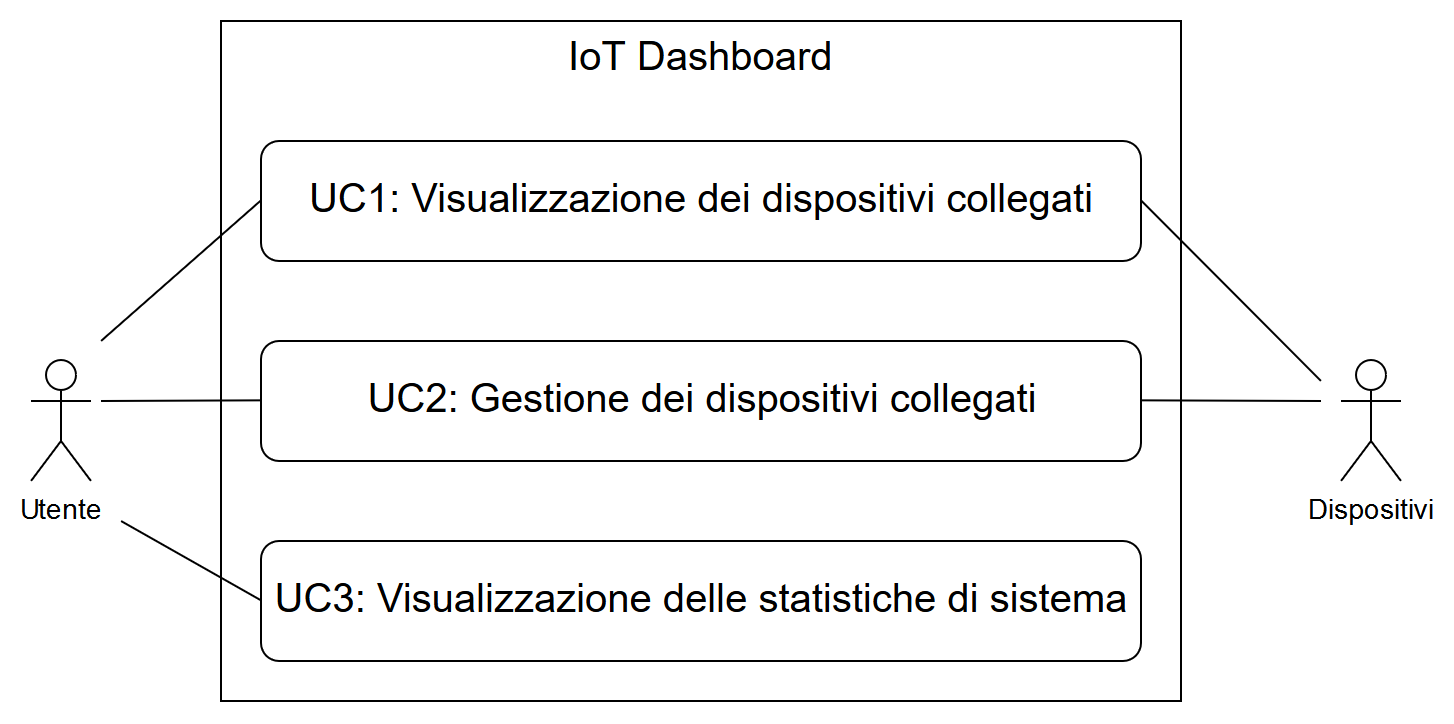
\includegraphics[width=0.9\columnwidth]{usecase/use_cases}
    \caption{Use Case - UC0: Scenario principale}
    \label{fig:scenario-principale}
\end{figure}
% fine uc

Durante le attività di analisi, ho utilizzato la tecnica del \emph{top down} a partire dallo scenario principale menzionato precedentemente per raggiungere, attraverso iterazioni in cui ho raffinato i problemi in sotto-problemi più specifici, uno stato in cui mi è risultato chiaro quali requisiti dovesse soddisfare il prototipo.
Per non allungare eccessivamente questa sezione, riporto l'analisi di uno dei casi d'uso sviluppati: la visualizzazione dei dispositivi collegati al sistema.
La visualizzazione dei dispositivi collegati, caso d'uso UC1 descritto testualmente in ~\ref{uc:uc1} e illustrato utilizzando il linguaggio UML in figura ~\ref{fig:uc1}, mette in relazione l'utente con i dispositivi collegati al sistema. Lo scopo di questa interazione è far conoscere all'utente alcune informazioni elementari riguardanti i dispositivi collegati. In questo caso d'uso ho incluso un'insieme di funzionalità che non cambiano lo scopo del caso d'uso, bensì specificano eventuali interazioni che l'utente può avviare con il sistema. Una delle particolarità del caso d'uso UC1 riguarda il modo con cui ho gestito l'interazione dell'utente con un singolo dispositivo (UC1.3): se l'utente interagisce con un singolo dispositivo nell'ambito di questo caso d'uso, allora l'utente desidera conoscere le informazioni che riguardano quel dispositivo in maggiore dettaglio. Dal momento che le informazioni presentate all'utente in questo \emph{step} riguardano i dispositivi collegati, allora significa che il dispositivo attore in UC1.3 è incluso nella lista dei dispositivi collegati. Da questo pensiero nasce la relazione di inclusione tra l'attore "Dispositivo" e l'attore più esteso "Dispositivi".

% uc testuale
\begin{usecase}{1}{Visualizzazione dei dispositivi collegati}
\usecaseactors{Utente, Dispositivi}
\usecasepre{L'utente ha scelto di visualizzare tutti i dispositivi collegati}
\usecasedesc{L'utente interroga la \emph{dashboard} per conoscere lo stato dei dispositivi collegati}
\usecasepost{L'utente conosce lo stato di tutti i dispositivi collegati al sistema}
\label{uc:uc1}
\end{usecase}

% uc figura
\begin{figure}[!h]
    \centering
    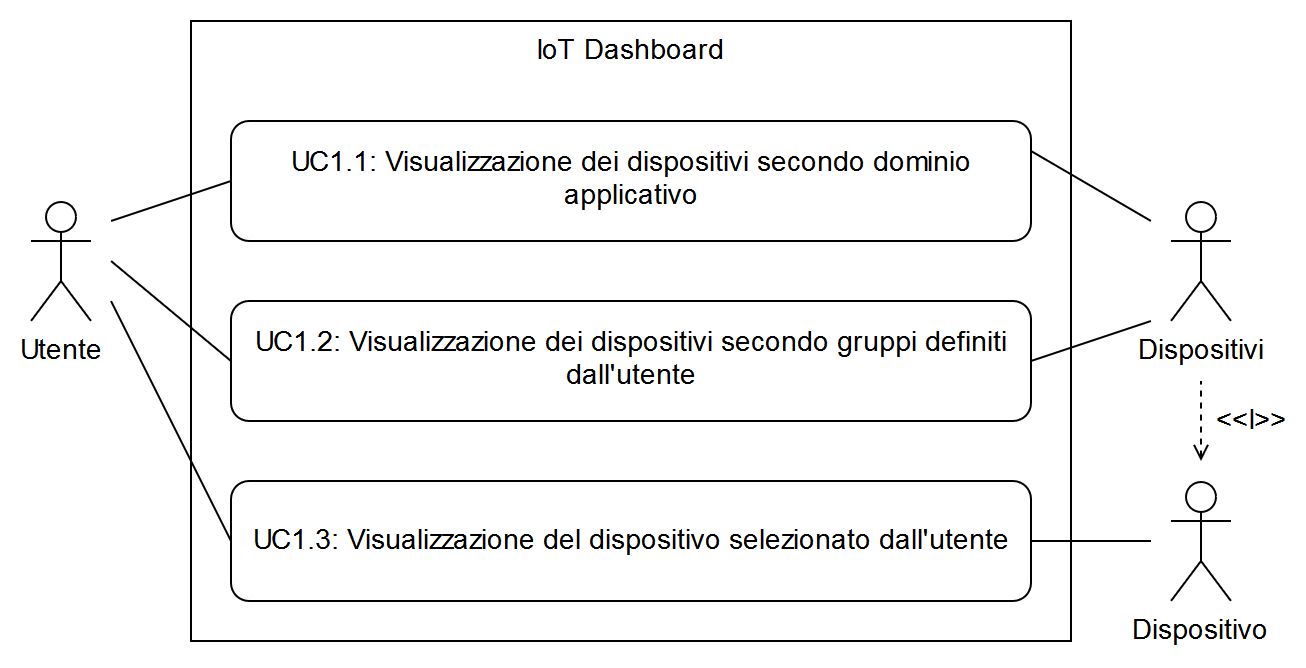
\includegraphics[width=0.9\columnwidth]{usecase/UC1}
    \caption{Use Case - UC1: Visualizzazione dei dispositivi collegati}
    \label{fig:uc1}
\end{figure}
% fine uc

% ## Requisiti
Presento di seguito i requisiti emersi durante l'analisi dei casi d’uso.
Per permetterne una consultazione agevole, ho deciso di inserire i requisiti in un insieme di tabelle dei requisiti suddivise in base alla categoria degli stessi.
In tutte le tabelle cui presenti presento i requisiti indicando:
\begin{itemize}
	\item Identificativo (secondo le regole indicate successivamente);
	\item Categoria di appartenenza fra:
	\begin{itemize}
		\item Obbligatorio, per i requisiti irrinunciabili;
		\item Desiderabile, per i requisiti non strettamente necessari ma che offrono un
    valore aggiunto riconoscibile;
		\item Opzionale, per i requisiti relativamente utili o contrattabili in seguito.
	\end{itemize}
	\item Descrizione esaustiva del requisito;
\end{itemize}
\smallskip

\newenvironment{conditions}
  {\par\vspace{\abovedisplayskip}\noindent\begin{tabular}{>{$}l<{$} @{${}={}$} l}}
  {\end{tabular}\par\vspace{\belowdisplayskip}}

% ### Catalogazione requisiti
Ho scelto di identificare i requisiti seguendo la forma seguente:

\begin{figure}[H]
  \centering
  \[ R[Categoria][Tipo][numero] \]
	dove
	\begin{conditions}
    R & specifica che si tratta di un requisito\\
    Categoria & indica se si tratta di un requisito tra quelli definiti in tabella ~\ref{tab:categoria-requisiti}\\
    Tipo & indica la tipologia del requisito tra quelli definiti in tabella ~\ref{tab:tipi-requisiti}\\
		Numero & è assoluto e rappresenta un riferimento univoco al requisito in questione\\
	\end{conditions}
\end{figure}

Per abbreviare le categorie utilizzate per identificare i requisiti ho associato nella tabella ~\ref{tab:categoria-requisiti} un identificativo a ciascuna categoria.

\begin{table}[H]
\caption{Tabella recante le categorie dei requisiti}
\label{tab:categoria-requisiti}
\begin{tabularx}{\linewidth}{|c|X|}
\hline
\textbf{Identificativo} & \textbf{Descrizione e origine} \\
\hline
M & Obbligatorio (\emph{mandatory}) \\
\hline
A & Desiderabile ((\emph{advisable}) \\
\hline
O & Opzionale (\emph{optional}) \\
\hline
\end{tabularx}
\end{table}

Nella tabella ~\ref{tab:tipi-requisiti} presento i tipi dei requisiti: il tipo indica l'origine del requisito e specifica se il requisito soddisfa una richiesta dell'utente del sistema oppure se esso deriva da una caratteristica del sistema.

\begin{table}[H]
\caption{Tabella recante i tipi dei requisiti}
\label{tab:tipi-requisiti}
\begin{tabularx}{\linewidth}{|c|X|}
\hline
\textbf{Identificativo} & \textbf{Descrizione e origine} \\
\hline
O & Di vincolo (\emph{obligation}) \\
\hline
F & Funzionale (\emph{functional}) \\
\hline
Q & Di qualità (\emph{quality}) \\
\hline
\end{tabularx}
\end{table}

% ### Tabella dei requisiti

% #### Tabella dei requisiti di vincolo
In tabella ~\ref{tab:requisiti-vincolo} indico i requisiti di vincolo che ho individuato durante le attività di analisi dei requisiti. Con questi requisiti indico i vincoli, tecnologici e non, che il sistema deve soddisfare al fine di realizzare un sistema efficiente nella sua implementazione\footnote{Con la locuzione efficienza nell'implementazione mi riferisco alla quantità di risorse spese per soddisfare i requisiti funzionali del sistema (ad es. quantità di tempo investito per l'implementazione delle funzionalità \emph{software}) rispetto al totale delle risorse allocate.}, nel funzionamento e nella manutenzione.

\begin{table}[H]
\caption{Tabella dei requisiti di vincolo}
\label{tab:requisiti-vincolo}
\begin{tabularx}{\linewidth}{|c|c|X|}
\hline
\textbf{Identificativo} & \textbf{Categoria} & \textbf{Descrizione} \\
\hline
RMO1 & Obbligatorio & Il sistema deve essere progettato secondo lo stile di progettazione a microservizi. \\
\hline
RAO2 & Desiderabile & Il sistema può essere implementato utilizzando il linguaggio JavaScript secondo lo standard ECMAScript 2017. \\
\hline
RAO3 & Desiderabile & Il sistema può essere implementato utilizzando il \emph{framework} Node.js per il \emph{backend} e React per il \emph{frontend}. \\
\hline
RMO4 & Obbligatorio & Il sistema deve utilizzare il protocollo MQTT. \\
\hline
\end{tabularx}
\end{table}

% #### Tabella dei requisiti funzionali
In tabella ~\ref{tab:requisiti-funzionali} indico i requisiti funzionali che ho individuato durante le attività di analisi dei requisiti. Con questi requisiti indico le funzionalità che il sistema deve offrire all'utente dello stesso e le classifico in base all'importanza che esse possono avere per l'utente che interagisce con il sistema.

\begin{table}[H]
\caption{Tabella dei requisiti funzionali}
\label{tab:requisiti-funzionali}
\begin{tabularx}{\linewidth}{|c|c|X|}
\hline
\textbf{Identificativo} & \textbf{Categoria} & \textbf{Descrizione} \\
\hline
RMF1 & Obbligatorio & L'utente deve poter visualizzare tutti i dispositivi collegati al sistema. \\
\hline
RMF2 & Obbligatorio & L'utente deve poter visualizzare i dispositivi collegati secondo dominio applicativo. \\
\hline
RAF3 & Desiderabile & L'utente può visualizzare i dispositivi collegati secondo gruppi personalizzati. \\
\hline
RMF4 & Obbligatorio & L'utente deve poter selezionare uno dei dispositivi collegati per visualizzarne le informazioni. \\
\hline
RAF5 & Desiderabile & L'utente può creare un gruppo di dispositivi personalizzato. \\
\hline
RAF6 & Desiderabile & L'utente può modificare uno dei gruppi personalizzati esistenti. \\
\hline
RAF7 & Desiderabile & L'utente può rimuovere uno dei gruppi di dispositivi personalizzati esistenti. \\
\hline
RMF8 & Obbligatorio & L'utente deve poter visualizzare le operazioni messe a disposizione dal dispositivo selezionato. \\
\hline
RMF9 & Obbligatorio & L'utente deve poter selezionare una delle operazioni disponibili. \\
\hline
RMF10 & Obbligatorio & L'utente deve poter visualizzare le statistiche di utilizzo del sistema sistema. \\
\hline
\end{tabularx}
\end{table}

% #### Tabella dei requisiti di qualità
In tabella ~\ref{tab:requisiti-qualita} indico i requisiti di qualità che ho individuato durante le attività di analisi dei requisiti. Con questi requisiti indico le caratteristiche che un sistema \emph{software} deve soddisfare per essere definito \emph{software} di qualità. Nel corso di Ingegneria del Software\footcite{swe-req-qual} ho studiato che i parametri con cui si può misurare la qualità di un \emph{software} possono essere suddivisi in due categorie:
\begin{itemize}
  \item i parametri esterni si riferiscono alla qualità del \emph{software} percepita dagli utenti (correttezza, affidabilità, efficienza, ecc.);
  \item i parametri interni si riferiscono alla qualità del \emph{software} percepita dagli autori del sistema e dai suoi manutentori (manutenibilità, riusabilità, leggibilità, ecc.).
\end{itemize}

\raggedbottom
\begin{table}[htbp]
\caption{Tabella dei requisiti di qualità}
\label{tab:requisiti-qualita}
\begin{tabularx}{\linewidth}{|c|c|>{\setlength\hsize{\hsize}}X|}
\hline
\textbf{Identificativo} & \textbf{Categoria} & \textbf{Descrizione} \\
\hline
ROQ1 & Opzionale & Il sistema deve essere testato, raggiungendo i seguenti obiettivi:
\begin{itemize}
	\item \emph{statement coverage} > 80 \%
	\item \emph{branch coverage} > 90 \%
\end{itemize}\\
\hline
\end{tabularx}
\end{table}

In tabella ~\ref{tab:requisiti-riepilogo} riepilogo i requisiti individuati in sede di analisi, suddividendoli in base al tipo e alla loro categoria d'importanza.

\begin{table}[htbp]
\caption{Tabella di riepilogo dei requisiti}
\label{tab:requisiti-riepilogo}
\begin{tabularx}{\linewidth}{|X|c|c|c|}
\hline
\textbf{Tipo} & \textbf{Obbligatorio} & \textbf{Opzionale} & \textbf{Desiderabile} \\
\hline
Funzionale & 6 & 0 & 4 \\
\hline
Qualitativo & 0 & 1 & 0 \\
\hline
Di vincolo & 2 & 0 & 2 \\
\hline
Totale & 8 & 1 & 6 \\
\hline
\end{tabularx}
\end{table}

\pagebreak

%**************************************************************
\section{Progettazione}
\label{progettazione}

% ### Scopo del documento

In questa sezione del documento definisco la progettazione dell'architettura ad alto livello del progetto di stage.
La sezione include la descrizione dell'architettura del sistema e delle relative componenti \emph{software} e i Design Pattern utilizzati per la progettazione.

L'architettura scelta per il sistema segue lo stile architetturale a microservizi con l'obiettivo di approfondire questo stile architetturale e implementarlo in uno scenario plausibile.
Lo stile architetturale a microservizi descrive un metodo di progettazione delle applicazioni come insiemi di servizi eseguibili indipendentemente, che comunicano tra loro grazie a meccanismi di comunicazione leggeri.
Nel mio caso, la comunicazione tra dispositivi avviene per mezzo del protocollo MQTT. Il protocollo MQTT si basa sul principio che ogni \emph{client} pubblica messaggi, i quali hanno uno o più argomenti, nel gergo tecnico \emph{topic}.
Ogni \emph{client} può registrarsi a determinati argomenti per ricevere tutti i messaggi che altri \emph{client} pubblicano per quell'argomento. Molti \emph{client} si connettono a un \gls{broker} che funziona da intermediario, ricevendo i messaggi pubblicati e inoltrandoli a tutti i \emph{client} sottoscritti ai rispettivi argomenti.
Gli argomenti in MQTT sono trattati gerarchicamente. Questo permette la creazione di argomenti e sottoargomenti, simili alla struttura ad albero di un \emph{filesystem}.
MQTT definisce 3 livelli di qualità della comunicazione in base a quanto \emph{broker} e \emph{client} si impegneranno a ricevere un messaggio.
I \emph{client} decidono il livello massimo di \gls{QoS} che riceveranno.
La scala della QoS definisce i livelli 0, 1 e 2 con affidabilità crescente ma minori performance:
\begin{itemize}
	\item [0]: \emph{broker} e/o \emph{client} invieranno il messaggio al massimo una volta senza richiesta di conferma. A questo livello i messaggi vengono persi se una delle parti si disconnette;
	\item [1]: \emph{broker} e/o \emph{client} invieranno il messaggio almeno una volta con la richiesta di conferma;
	\item [2]: \emph{broker} e/o \emph{client} invieranno il messaggio una sola volta effettuando una trasmissione in 4 step.
\end{itemize}

Per esempio, se un messaggio è pubblicato con QoS 2 e il \emph{client} è sottoscritto all'argomento con QoS 0, il \emph{client} riceverà quel messaggio con QoS 0 (niente richieste di conferma, ecc).
Se un altro \emph{client} è sottoscritto allo stesso argomento con QoS 2 allora riceverà il messaggio con QoS 2 (\gls{handshake} in 4 step).
Alla connessione il \emph{client} imposta un parametro logico che rappresenta una "sessione pulita" in base a come il \emph{client} ritiene affidabile la connessione (`false` indica una connessione affidabile). Se il \emph{client} si disconnette, in tutte le sottoscrizioni con QoS 1 o QoS 2 i messaggi verranno salvati e inviati alla prossima riconnessione del \emph{client}.

Ho progettato le componenti del sistema seguendo il paradigma orientato agli oggetti: in questo modo ho potuto organizzare il codice in moduli riutilizzabili dalle diverse componenti del \emph{software}, diminuendo la possibilità che implementi funzionalità comuni in moduli diversi e con comportamento diverso che potrebbe causare malfunzionamenti nel sistema.
Le attività di progettazione ad alto livello del sistema hanno richiesto da parte mia la redazione di un documento di Specifica Tecnica del sistema, nel quale ho indicato:
\begin{itemize}
  \item le tecnologie e gli strumenti utilizzati;
  \item una panoramica dell'architettura del sistema;
  \item gli approfondimenti riguardanti le componenti definite all'interno dei servizi che compongono il sistema;
  \item i Design Pattern utilizzati all'interno delle componenti dei servizi del sistema.
\end{itemize}

Durante la progettazione delle componenti del prototipo ho utilizzato i diagrammi UML delle classi per rappresentare i tipi delle entità ed evidenziare le relazioni tra queste: in questo modo ho individuato le dipendenze tra le entità e sono quindi stato in grado di modularizzare alcune funzionalità in componenti isolate e riutilizzabili.
Per snellire la procedura di inserimento della specifica delle classi all'interno della Specifica Tecnica ho utilizzato \emph{template}.

Nell'immagine ~\ref{img:overview-arch} illustro la panoramica delle componenti di cui è composta l'architettura utilizzando la notazione dei diagrammi delle componenti UML.

\begin{figure}[H]
    \centering
    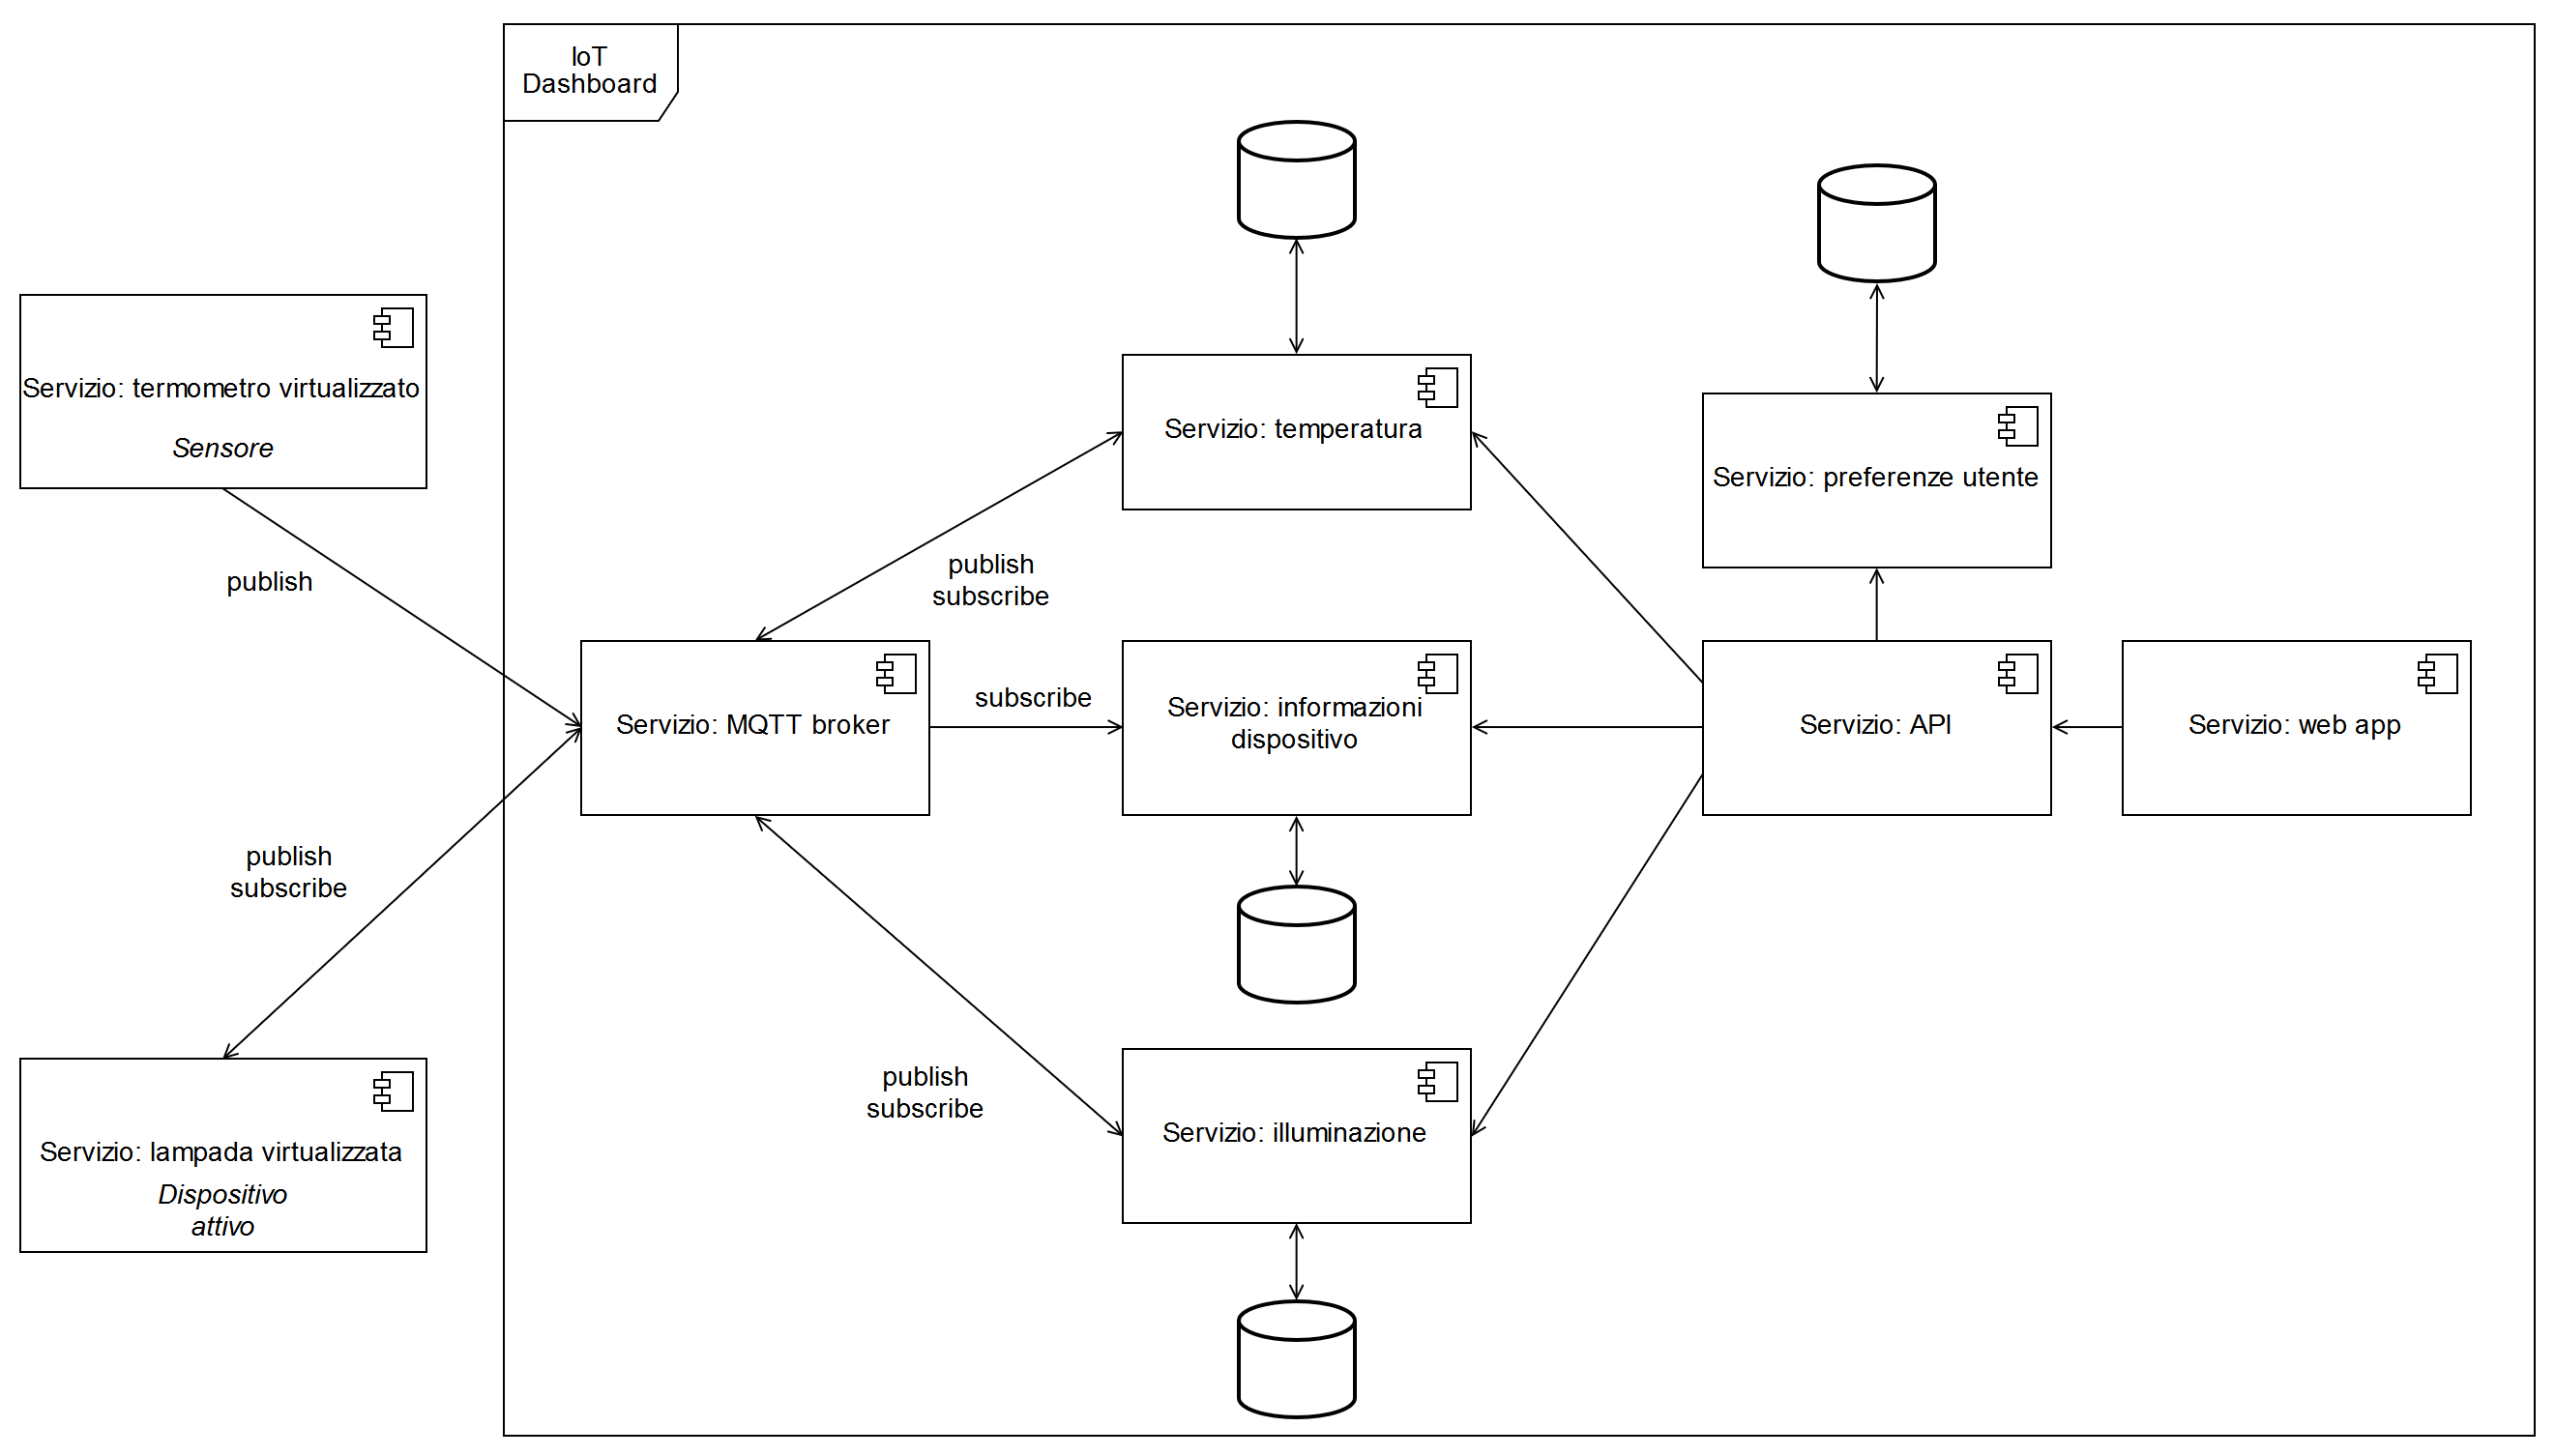
\includegraphics[width=\columnwidth]{progettazione/arch-overview}
    \caption{Panoramica dell'architettura ad alto livello progettata per il prototipo}
    \label{img:overview-arch}
\end{figure}

% ### Servizio: MQTT \emph{broker}
Il \emph{broker} MQTT è il servizio responsabile alla ricezione di tutti i messaggi, alla loro catalogazione e all'invio delle notifiche verso i \emph{client} sottoscritti a ciascuna categoria.
Il \emph{broker} memorizza lo stato di tutti i \emph{client} a lui connessi, inclusi i messaggi non ancora inviati o il cui invio è fallito.

% ### Servizio: termometro _virtualizzato_
Il termometro "virtualizzato" è il servizio responsabile della simulazione di un sensore che invii dati sulla temperatura dell'ambiente in cui si trova.
Esso pubblica periodicamente la temperatura rilevata secondo l'argomento \emph{temperature}, mentre invia secondo l'argomento \emph{hw\_info} i propri dati identificativi, quali produttore, modello, ecc..
Data la relativa importanza i dati vengono inviati con un QoS di livello 0 nella categoria \emph{temperature}, mentre con QoS di livello 1 nella categoria \emph{hw\_info}.
In questo modo al collegamento del dispositivo "virtualizzato" viene effettuato almeno un tentativo di trasmissione delle informazioni relative alle specifiche del dispositivo.
Anche se nel diagramma è disegnato individualmente, è possibile che ve ne siano molteplici.
Nel diagramma ~\ref{fig:classi-termometro} ho illustrato il diagramma delle classi UML a cui sono giunto durante le attività di progettazione ad alto livello. Vista la necessità di generare dati riguardanti la temperatura in maniera pseudocasuale, ho utilizzato il Design Pattern \gls{abstract-factory} per permettere la creazione di funzioni per la generazione della temperatura. Queste funzioni per la generazione della temperatura sono incapsulate in una classe \texttt{TemperatureCurve}, il cui scopo è definire la funzione matematica che restituisce la temperatura in base alla data e ora specificata. L'implementazione di \texttt{TemperatureCurve} progettata per il termometro virtualizzato è \texttt{SineTemperatureCurve}, nella quale restituisco la temperatura sulla base di una temperatura di base specificata e applicando a tale temperatura una funzione sinusoidale.
Ho applicato il Design Pattern Abstract Factory definendo una classe \texttt{TemperatureCurveFactory}, il cui unico scopo è creare oggetti che implementino \texttt{TemperatureCurve}.
Nella tabella ~\ref{tab:classi-termometro} ho elencato le classi sviluppate per soddisfare i requisiti di funzionamento del dispositivo.

\begin{figure}[!h]
    \centering
    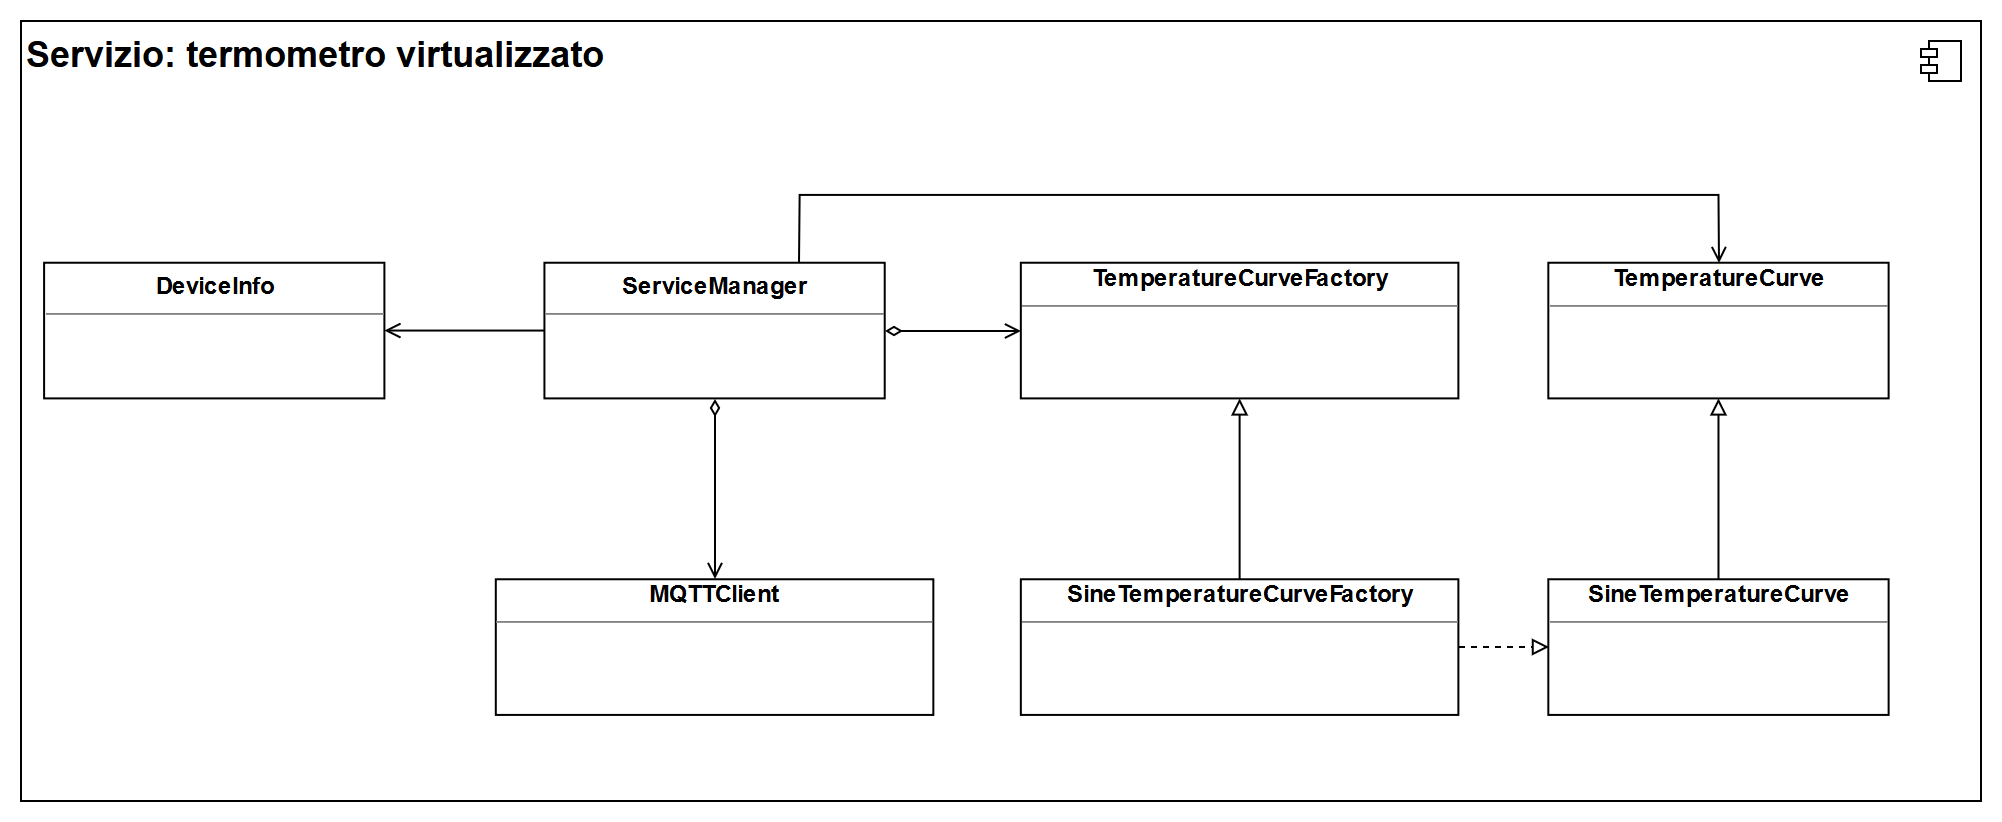
\includegraphics[width=\columnwidth]{progettazione/virtual_temp_sensor_classes}
    \caption{Architettura ad alto livello progettata per il termometro virtualizzato}
    \label{fig:classi-termometro}
\end{figure}

\begin{table}[!h]
\caption{Panoramica delle classi del servizio di simulazione del termometro}
\label{tab:classi-termometro}
\begin{tabularx}{\linewidth}{|c|X|}
\hline
\textbf{Classe} & \textbf{Funzionalità} \\
\hline
\texttt{DeviceInfo} & Classe che indica le informazioni del dispositivo (produttore, modello, revisione, ecc.) pubblicate nel \emph{topic} \emph{hw\_info}.\\
\hline
\texttt{ServiceManager} & Classe responsabile dell'integrazione tra generazione dei dati di temperatura, gestione delle informazioni del dispositivo e invio delle informazioni tramite protocollo MQTT. \\
\hline
\texttt{MQTTClient} & Classe utile all'inizializzazione del \emph{client} MQTT. \\
\hline
\texttt{TemperatureCurveFactory} & Classe Factory che espone la funzionalità di creazione della curva di temperatura, rappresentata dalla classe \texttt{TemperatureCurve}. \\
\hline
\texttt{SineTemperatureCurveFactory} & Implementazione della factory \texttt{TemperatureCurveFactory} per la creazione di oggetti \texttt{SineTemperatureCurve}. \\
\hline
\texttt{TemperatureCurve} & Classe che espone le funzionalità di creazione di una funzione, di aggiunta di rumore pseudocasuale nella funzione creata e di simulazione della temperatura data l'ora corrente. \\
\hline
\texttt{SineTemperatureCurve} & Classe che implementa \texttt{TemperatureCurve} definendo una funzione di simulazione sinusoidale parametrizzabile in ampiezza, frequenza e fase. \\
\hline
\end{tabularx}
\end{table}

% ### Servizio: temperatura
Il servizio relativo alla temperatura si occupa di raccogliere tutti i dati provenienti dai sensori di temperatura, memorizzandoli e mettendoli a disposizione in un formato strutturato per gli altri servizi del sistema.
Il servizio si sottoscrive alla categoria \emph{temperature} e comunica con un QoS di livello 0, inoltre può pubblicare messaggi con la sotto-categoria \emph{temperature/active} per usufruire delle funzionalità aggiuntive presenti in dispositivi attivi legati alla temperatura, con un QoS di livello 1.

% Lampada virtualizzata
Con il servizio della lampada "virtualizzata" simulo la presenza nella rete di un dispositivo "attivo": una lampada in grado di comunicare il proprio assorbimento energetico e che è controllabile da remoto.
La lista delle operazioni disponibili è la seguente:
\begin{itemize}
	\item accensione della lampada (QoS di livello 2);
	\item spegnimento della lampada (QoS di livello 2);
	\item richiesta assorbimento energetico (QoS di livello 0);
\end{itemize}
Le operazioni di accensione e spegnimento della lampada necessitano di una affidabilità più elevata delle altre operazioni per evitare l'invio di richieste di accensione e spegnimento multiple.
L'argomento a cui la lampada si sottoscrive è \emph{light/active} e al primo collegamento la lampada invia i propri dati identificativi, pubblicandoli nella categoria \emph{hw\_info}.

% ### Servizio: illuminazione
Il servizio relativo all'illuminazione si occupa di raccogliere e memorizzare tutti i dati pubblicati dai dispositivi nella categoria \emph{light} e permette il controllo dei dispositivi sottoscritti alla categoria \emph{light/active}.
Questo servizio utilizza trasmissioni con tutti i livelli di QoS definiti nel protocollo MQTT: la comunicazione delle operazioni che l'utente esegue vengono trasmessi con il livello di affidabilità maggiore (QoS livello 2) per avere la garanzia che i dati trasmessi siano arrivati ai dispositivi atomicamente, la trasmissione delle specifiche tecniche del dispositivo vengono inviate con un livello di affidabilità intermedio (QoS livello 1) mentre le misurazioni vengono inviate nel modo più efficiente possibile (QoS livello 0).

% ### Servizio: informazioni dispositivo
Il servizio relativo alle informazioni dei dispositivi si occupa di raccogliere e memorizzare tutti i dati pubblicati secondo l'argomento \emph{hw\_info}; utilizza esclusivamente un livello di QoS pari a 1 per aumentare l'affidabilità del sistema a fronte delle attività di identificazione dei dispositivi collegati.

% ### Servizio: preferenze utente
Il servizio di gestione delle preferenze utente si occupa di salvare informazioni quali ad esempio gruppi personalizzati, unità di misura preferite, ecc.
Il servizio non utilizza il protocollo MQTT in quanto non richiede la comunicazione con i dispositivi connessi alla rete, quindi viene utilizzato solamente dal servizio API.

% ### Servizio: API
Il servizio API svolge un ruolo da intermediario tra il servizio che fornisce l'applicazione \emph{web} e i microservizi che raccolgono i dati dei dispositivi.
Esso interroga i servizi "illuminazione", "temperatura" e "informazioni dispositivo"  definiti dal sistema per fornire una interfaccia unificata ai dati.
Per la progettazione del servizio API ho utilizzato uno dei Design Pattern specifici per le architetture a microservizi, ossia il \emph{Gateway Pattern}.
Ho progettato il servizio API in modo \emph{stateless} grazie alla composizione delle API esposte dagli altri servizi: le chiamate effettuate al servizio API vengono dirottate ai rispettivi servizi e opportunamente decorate con informazioni aggiuntive, utili durante le attività di \emph{debug} del prototipo.

% ### Servizio: web app
Il servizio "\emph{web app}" comprende l'applicazione \emph{web} per la consultazione della \emph{dashboard} e include le componenti sviluppate in React per la costruzione dell'interfaccia grafica della \emph{dashboard} e le classi necessarie alla sua pubblicazione sul \emph{web}.
Per conferire un elevato grado di riutilizzabilità ai componenti creati ho utilizzato il Design Pattern \gls{dp-composite} (rappresentato in figura ~\ref{fig:composite}): nella progettazione dell'interfaccia ho individuato dapprima componenti elementari che estendono la classe \texttt{React.Component} (ad esempio componenti per visualizzare il testo specificato) e gradualmente ho assemblato componenti più complesse, sempre estensioni della classe \texttt{React.Component} (ad esempio unendo la componente di visualizzazione del testo con la componente di visualizzazione di una immagine). Attraverso questo procedimento \emph{bottom up} ho concluso la progettazione delle componenti dell'interfaccia, giungendo alla componente \texttt{UIPage}, la quale è anch'essa una componente React che specifica quali componenti e con quale struttura visualizzare a schermo una determinata pagina. Ciascuna pagina dell'applicazione \emph{web} è quindi un \emph{collage} di componenti più o meno complesse che mi hanno permesso di riutilizzare i componenti elementari in molte pagine dell'applicazione.

\begin{figure}[H]
    \centering
    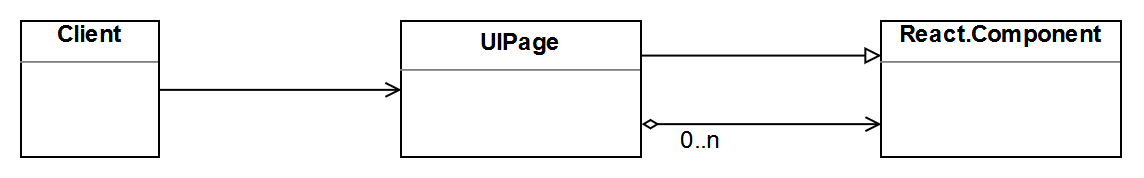
\includegraphics[width=0.95\columnwidth]{progettazione/composite}
    \caption{Rappresentazione semplificata del Design Pattern Composite}
    \label{fig:composite}
\end{figure}

Nel diagramma ~\ref{fig:classi-web} indico l'architettura ad alto livello progettata per il servizio di presentazione delle informazioni e nella tabella ~\ref{tab:classi-web} descrivo le classi sviluppate.

\begin{figure}[H]
    \centering
    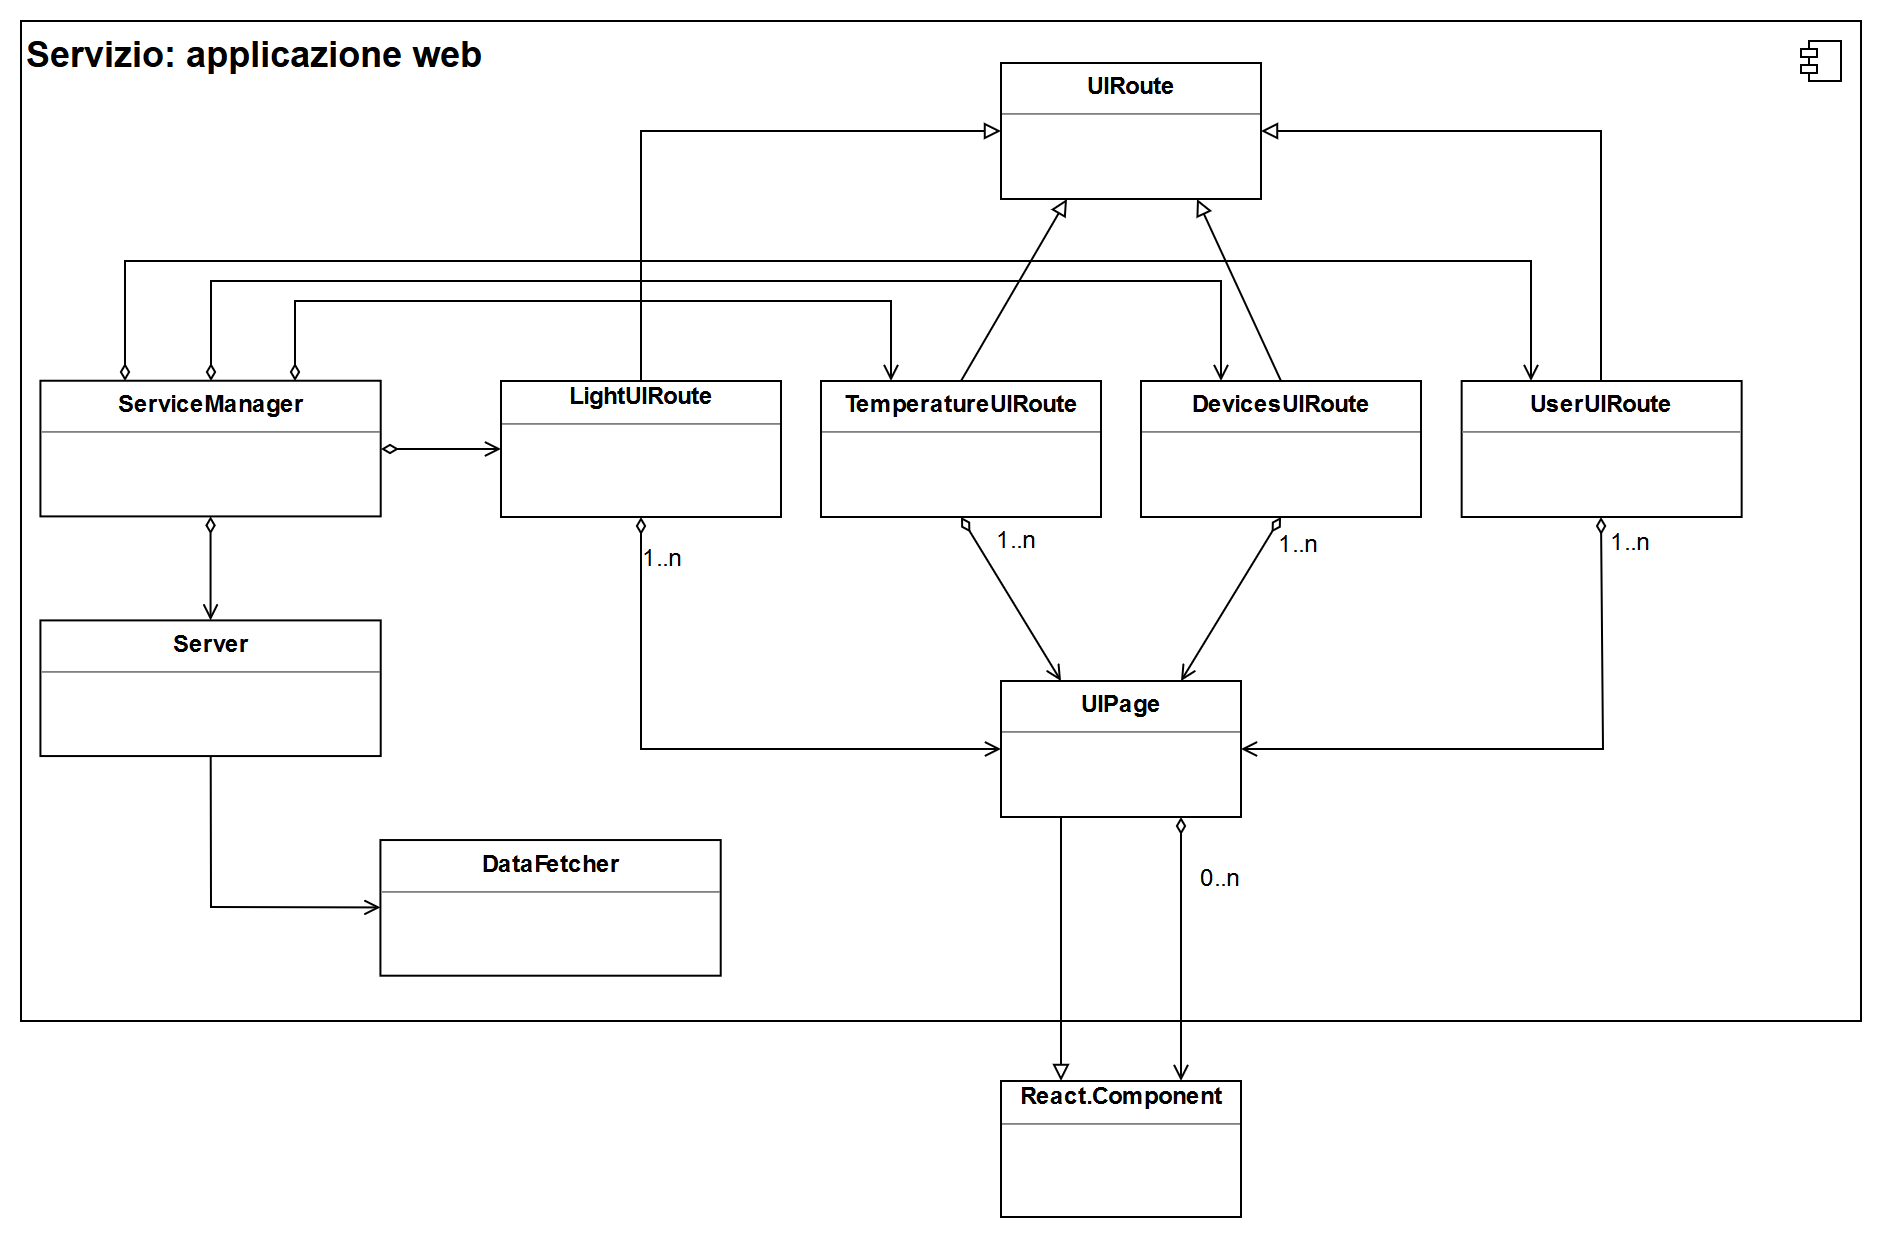
\includegraphics[width=0.90\columnwidth]{progettazione/web_service_classes}
    \caption{Architettura ad alto livello progettata per il servizio \emph{web app}}
    \label{fig:classi-web}
\end{figure}

\begin{table}[htbp]
\caption{Panoramica delle classi del servizio API}
\label{tab:classi-web}
\begin{tabularx}{\linewidth}{|c|X|}
\hline
\textbf{Classe} & \textbf{Funzionalità} \\
\hline
\texttt{ServiceManager} & Classe responsabile dell'integrazione tra istanza del server, pagine esposte e interfaccia di richiesta dati. \\
\hline
\texttt{DataFetcher} & Modulo che si occupa di effettuare le richieste al servizio API secondo le definizioni fornite dal servizio. \\
\hline
\texttt{Server} & Classe responsabile del ciclo di vita del server Node.js. Effettua le richieste definite dalle istanze di \texttt{UIRoute} per ricevere i dati, utilizzando un'istanza di \texttt{DataFetcher}. \\
\hline
\texttt{UIRoute} & Interfaccia utilizzata per definire le richieste da effettuare per ricevere le informazioni che popolano le pagine della rotta. \\
\hline
\texttt{UserUIRoute} & Implementazione di \texttt{UIRoute} che definisce le richieste per ottenere o modificare le preferenze dell'utente ed espone le pagine di visualizzazione e modifica delle preferenze utente. \\
\hline
\texttt{DevicesUIRoute} & Implementazione di \texttt{UIRoute} che definisce le richieste per ottenere informazioni sui dispositivi collegati ed espone le pagine di visualizzazione di questi. \\
\hline
\texttt{TemperatureUIRoute} & Implementazione di \texttt{UIRoute} che definisce le richieste per ottenere dati legati alla temperatura, visualizzare ed eseguire operazioni con dispositivi attivi e ne permette la visualizzazione. \\
\hline
\texttt{LightUIRoute} & Implementazione di \texttt{UIRoute} che definisce le richieste per ottenere dati legati all'illuminazione, visualizzare ed eseguire operazioni con dispositivi attivi e ne permette la visualizzazione. \\
\hline
\texttt{UIPage} & Implementazione di un componente React (\texttt{React.Component}) che rappresenta una pagina. La pagina visualizzata può contenere più figli anch'essi componenti React. \\
\hline
\texttt{React.Component} & Classe che rappresenta una componente grafica nel \emph{framework} React. \\
\hline
\end{tabularx}
\end{table}

\pagebreak

%**************************************************************
\section{Implementazione e verifica}

Durante le attività di implementazione delle specifiche del sistema ho scritto, oltre al codice sorgente dei servizi, anche documenti in cui indico le istruzioni per eseguire le singole componenti del sistema e specifico le risorse esposte dalle stesse.
I documenti in cui indico le risorse esposte dai servizi sono rivolti agli utenti più esperti che vogliono approfondire le funzionalità offerte dai servizi. Nelle mie previsioni questi utenti grazie ai documenti di specifica dovrebbero essere in grado di implementare le altre componenti del sistema, sostituendo le componenti da me implementate. Ho scritto questi documenti contestualmente all'implementazione delle funzionalità nel codice sorgente, adeguandoli manualmente ad ogni modifica compiuta nel codice sorgente.\\
Ho deciso di scrivere i documenti in cui indico le istruzioni per eseguire il progetto sia in lingua italiana, sia in lingua inglese dal momento che il progetto è disponibile pubblicamente su GitHub. Nel farlo ho seguito alcuni consigli che ho tratto dalla lista degli articoli presenti al link \url{https://github.com/matiassingers/awesome-readme\#articles}: in questo \gls{repository} l'autore ha raccolto collegamenti a:
\begin{itemize}
  \item esempi di pagine informative dei rispettivi progetti caratterizzate da una buona struttura e da contenuti adeguati agli utenti a cui questi progetti sono indirizzati;
  \item articoli di autori che espongono la loro opinione riguardo a come dovrebbero essere scritti i documenti che gli utenti devono leggere in sede di esplorazione del progetto;
  \item strumenti che facilitano la scrittura dei documenti informativi.
\end{itemize}
Nelle istruzioni ho incluso i riferimenti per installare i \emph{software} richiesti e ho fatto in modo che i procedimenti da seguire fossero i più brevi possibili (procedimenti con al massimo 5 istruzioni da seguire). Ho scritto queste istruzioni solamente quando mi sono accertato che le componenti fossero abbastanza stabili nel loro funzionamento da poter essere potenzialmente usate da altri utenti.\\
Ho scritto la documentazione del codice sorgente contestualmente al codice sorgente; la documentazione del codice sorgente consiste in commenti nei sorgenti JavaScript in cui spiego:
\begin{itemize}
	\item lo scopo delle proprietà degli oggetti;
	\item il tipo delle proprietà degli oggetti: in questo caso ho preferito annotare il tipo delle proprietà degli oggetti nella documentazione in quanto JavaScript non è staticamente tipizzato e quindi la dichiarazione di variabili non consente di specificare un tipo con cui il compilatore e l'interprete validino il codice sorgente;
	\item gli algoritmi utilizzati per l'implementazione delle funzionalità.
\end{itemize}
Ho scritto i commenti nel codice sorgente, come da \emph{best practice} per i progetti distribuiti pubblicamente, in lingua inglese.

Prima di iniziare le attività di codifica ho utilizzato Yeoman (\url{http://yeoman.io/}) per generare un \emph{template} che ho utilizzato per implementare tutti i servizi. Nel \emph{template} ho specificato le dipendenze comuni a tutti i servizi e ho configurato la struttura dei progetti in modo che fosse ripetibile per tutti i servizi.
Ogni servizio, grazie alla generazione per mezzo del \emph{template}, ha al suo interno gli strumenti di analisi statica e dinamica del codice, un documento di \emph{README} contenente le informazioni specifiche per il servizio e un \emph{Dockerfile} responsabile della creazione dei \emph{container}.
Lo strumento principale che ho utilizzato durante la codifica è l'\emph{editor} Visual Studio Code, indicato in tabella ~\ref{tab:strumenti}, grazie al quale ho utilizzato gli strumenti di analisi statica e dinamica del codice durante la sua scrittura.

Le attività di verifica garantiscono che l'esecuzione delle attività pianificate nel corso dello svolgimento di un progetto non introducano errori.
Durante le attività di verifica dei requisiti ho controllato la loro consistenza e la loro completezza, accertandomi che fossero chiaramente definiti, tuttavia ho tralasciato il controllo della loro realizzabilità confidando nelle mie capacità implementative.
Durante le attività di progettazione ad alto livello del prototipo ho iterato le attività di verifica sui diagrammi delle classi UML al fine di verificare che essi rispondessero a due criteri:
\begin{itemize}
  \item il grado di accoppiamento medio delle classi, calcolato come differenza in valore assoluto tra le relazioni in ingresso e le relazioni in uscita per ogni classe, sia nell'intervallo [0, 2] (ogni classe può utilizzare in media fino a un massimo di due altre classi);
  \item le classi all'interno di ciascun microservizio offrano le funzionalità essenziali per soddisfare i requisiti correlati e non dipendano dagli altri servizi per funzionare.
\end{itemize}
Ai due criteri ho associato gradi di importanza non equivalenti: ho preferito concentrarmi sul secondo criterio, che ho potuto applicare a tutti i servizi ad eccezione del servizio API intermediario con i \emph{client}) per acquisire esperienza nell'applicazione del concetto \emph{micro} ai servizi richiesto dalle architetture a microservizi.
Ho svolto le attività di verifica durante l'implementazione del \emph{software} da due lati:
\begin{itemize}
  \item ho pianificato il primo insieme di attività del processo di verifica del prodotto utilizzando gli strumenti di analisi statica per prevenire errori comuni e facilmente risolvibili automaticamente;
  \item ho pianificato il secondo insieme di attività del processo di verifica del prodotto effettuando prove durante l'esecuzione del \emph{software}.
\end{itemize}
Ho condotto l'analisi dinamica del prodotto sia con l'ausilio di strumenti di test automatici, sia effettuando prove manuali, simulando l'interazione di un \emph{client}, inteso come attore, con i servizi.
Ho progettato i test per raggiungere la copertura del codice fissata durante l'attività di Analisi dei requisiti (riferimento ~\ref{tab:requisiti-qualita}).
Durante la progettazione dei test ho scelto di approfondire la progettazione dei test d'unità di tutte le componenti progettate come primo \emph{step} mentre ho tralasciato la progettazione dei test d'integrazione dei servizi: ho perseguito questa scelta perché ho ritenuto più importante aumentare l'affidabilità intrinseca di ciascun servizio indipendentemente dagli altri.
Uno dei fattori che mi ha consentito di effettuare questa scelta consiste nell'individualità dell'implementazione del progetto: se al progetto avessero collaborato uno o più sviluppatori, avrebbe assunto maggiore importanza la corretta interazione tra i servizi. Inoltre, dal momento che i servizi che ho progettato hanno un flusso dei dati ben definito, mi ha permesso di tenere allineate le modifiche attraverso i servizi in efficienza.
Nei test ho usato ampiamente \emph{mock} e \emph{stub} per isolare le eventuali dipendenze tra un modulo e un altro all'interno dello stesso servizio. Come avevo previsto durante lo studio degli argomenti, la componente in cui ho avuto alcune difficoltà nell'implementazione dei test consiste nei moduli che dialogano con un \emph{database}: per arginare il problema ho utilizzato librerie accessorie presenti su npm per simulare le risposte che i \emph{database} inviano nel caso in cui si verifichino errori. In questo modo ho potuto testare con successo anche eventuali malfunzionamenti relativi al collegamento con i \emph{database}.
Ho elencato i risultati della copertura del codice raggiunta al termine dello stage nella tabella ~\ref{tab:coverage}.

\begin{table}[H]
\caption{Tabella che specifica la copertura del codice raggiunta per ciascun servizio}
\label{tab:coverage}
\begin{tabularx}{\linewidth}{|X|c|c|}
\hline
\textbf{Servizio} & \textbf{\emph{Statement coverage}} & \textbf{\emph{Branch coverage}} \\
\hline
MQTT Broker & 93 \% & 90 \% \\
\hline
Sensore di temperatura "virtualizzato" & 97 \% & 85 \% \\
\hline
Temperatura & 92 \% & 81 \% \\
\hline
Lampada \emph{smart} "virtualizzata" & 83 \% & 67 \% \\
\hline
Illuminazione & 91 \% & 65 \% \\
\hline
Informazioni dispositivi & 90 \% & 77 \% \\
\hline
Preferenze utente & 90 \% & 79 \% \\
\hline
API & 70 \% & 70 \% \\
\hline
Applicazione \emph{web} & 50 \% & 63 \% \\
\hline
\textbf{Totale} & 85,44 \% & 75,22 \% \\
\hline
\end{tabularx}
\end{table}

%**************************************************************
\section{Validazione dei requisiti}
\label{val-req}

Nella tabella ~\ref{tab:validazione-requisiti}) ho elencato lo stato dell'implementazione dei requisiti citati in Analisi (riferimento ~\ref{ar})).

\begin{table}[H]
\caption{Tabella dei requisiti funzionali}
\label{tab:validazione-requisiti}
\begin{tabularx}{\linewidth}{|c|c|X|}
\hline
\textbf{Identificativo} & \textbf{Categoria} & \textbf{Esito} \\
\hline
RMF1 & Obbligatorio & Soddisfatto \\
\hline
RMF2 & Obbligatorio & Soddisfatto \\
\hline
RAF3 & Desiderabile & Omesso \\
\hline
RMF4 & Obbligatorio & Soddisfatto \\
\hline
RAF5 & Desiderabile & Omesso. \\
\hline
RAF6 & Desiderabile & Omesso. \\
\hline
RAF7 & Desiderabile & Omesso \\
\hline
RMF8 & Obbligatorio & Soddisfatto \\
\hline
RMF9 & Obbligatorio & Soddisfatto \\
\hline
RMF10 & Obbligatorio & Parzialmente soddisfatto \\
\hline
ROQ1 & Opzionale & Soddisfatto \\
\hline
RMO1 & Obbligatorio & Soddisfatto \\
\hline
RAO2 & Desiderabile & Soddisfatto \\
\hline
RAO3 & Desiderabile & Soddisfatto \\
\hline
RMO4 & Obbligatorio & Soddisfatto \\
\hline
\end{tabularx}
\end{table}

Durante lo svolgimento dello stage ho deciso di non implementare i requisiti relativi alla personalizzazione dei gruppi di dispositivi perché ho incontrato alcune difficoltà relative alla composizione dei servizi che hanno rallentato l'implementazione delle funzionalità dei servizi. Come avevo previsto in sede di valutazione dei rischi (riferimento ~\ref{tab:rischi-arch-microservizi}), la difficoltà nel reperimento delle informazioni correlate ad esempi pratici delle architetture a microservizi ha causato un generale rallentamento delle attività di sviluppo.
In particolare, ho avuto difficoltà in due momenti:
\begin{itemize}[nosep]
  \item durante lo sviluppo di una soluzione sperimentale che permettesse di utilizzare la tecnica dello \gls{sharding} tra molteplici \emph{database} in un contesto di utilizzo basato sui \emph{container};
  \item durante lo sviluppo del servizio di integrazione delle API (servizio API citato in ~\ref{progettazione}) fornite dai singoli microservizi.
\end{itemize}
Ho riscontrato la prima problematica a causa della documentazione legata allo \emph{sharding} del \emph{database} considerato: dal momento che essa è indirizzata per installazioni dei \emph{database} direttamente sui calcolatori ho avuto difficoltà a trasportare quelle istruzioni nell'ambito della composizione di \emph{container}, richiedendo una quantità superiore a quella che avevo valutato per essere implementata.\\
Proseguendo con la seconda criticità, questa si è verificata a causa di una mia incomprensione del meccanismo di condivisione della rete nell'ambito dell'orchestrazione dei servizi attraverso Docker Compose: nella pratica i servizi legati alla temperatura, all'illuminazione, alla gestione delle informazioni dei dispositivi e alle preferenze utente potevano essere interrogati individualmente, tuttavia non riuscivano a comunicare con il servizio di integrazione (servizio API) perché Docker Compose internamente isolava i \emph{container} in sotto-reti virtuali senza possibilità di comunicare tra loro. Ho risolto il problema definendo manualmente una nuova sotto-rete virtuale, comune a tutti i servizi, che ha permesso al sistema di funzionare correttamente.\\
Per quanto riguarda il requisito RMF10, relativo alla visualizzazione delle statistiche di sistema, ho deciso di implementare solamente la componente di controllo della salute dei servizi che compongono il sistema \emph{healthcheck}, tralasciando le componenti di integrazione dei dati raccolti dai servizi e le componenti di visualizzazione dei dati citati.\\
A causa dei rallentamenti menzionati ho scelto di non implementare alcune funzionalità perché, sebbene le avessi catalogate come desiderabili, la quantità di risorse rimanenti non sarebbe stata sufficiente alla loro corretta implementazione, quindi ho preferito allocare tempo per migliorare la qualità del \emph{software} sviluppato aumentando la copertura del codice sorgente, implementando un numero maggiore di test di unità. Mi è ora chiaro che alcuni dei requisiti da me classificati avrebbero richiesto ulteriori passaggi di verifica: la fattibilità e la valutazione più attenta del rapporto importanza della funzionalità paragonato alle risorse a disposizione avrebbero evidenziato che alcuni requisiti non erano implementabili nelle ore destinate al progetto di stage.
             % Kick-Off
% !TEX encoding = UTF-8
% !TEX TS-program = pdflatex
% !TEX root = ../relazione-finale.tex

%**************************************************************
\pagebreak
\chapter{Valutazione retrospettiva}
\label{cap:analisi-requisiti}
%**************************************************************

\section{Presentazione \emph{dashboard}}

Ho composto l'interfaccia grafica della \emph{dashboard} di due parti:
\begin{itemize}
  \item una barra verticale sulla sinistra contenente le voci di navigazione del menù;
  \item la restante parte della pagina per la visualizzazione dei contenuti.
\end{itemize}
Come illustro in figura ~\ref{fig:homepage}, nella pagina principale della \emph{dashboard} presento lo stato dei servizi del sistema: per ogni servizio mostro il nome, un icona di riconoscimento e, per mezzo di un pallino verde o rosso, il suo stato (operativo o malfunzionante).

\begin{figure}[!h]
    \centering
    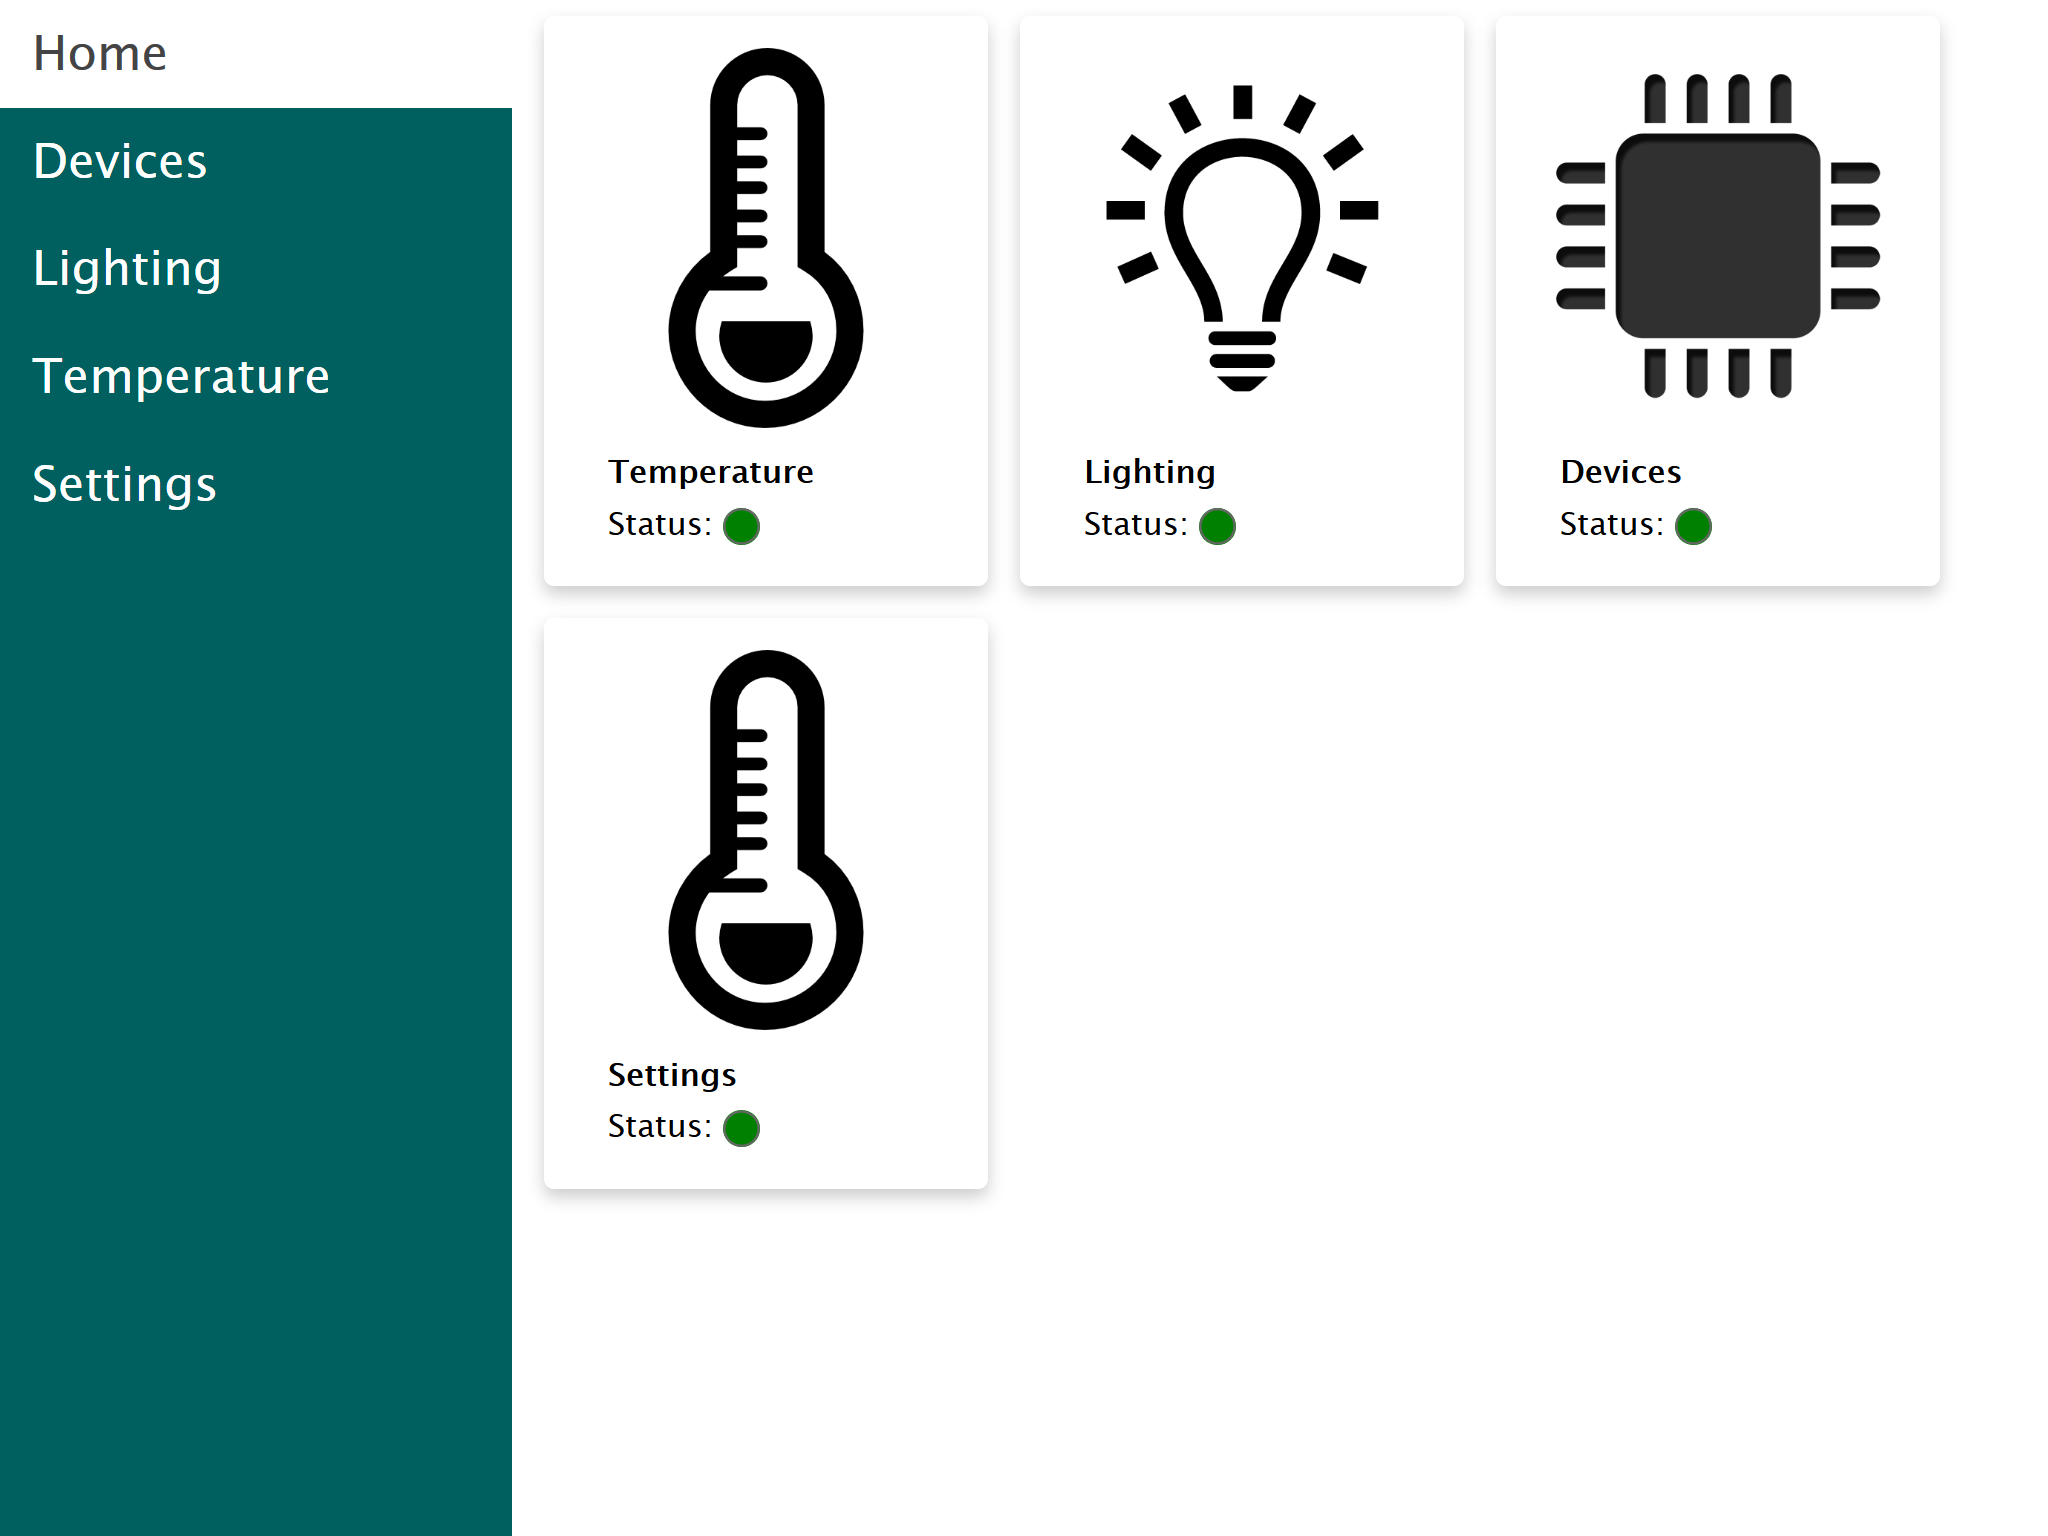
\includegraphics[width=0.9\columnwidth]{demo/home-page}
    \caption{Pagina principale della \emph{dashboard}}
    \label{fig:homepage}
\end{figure}

Navigando nella pagina dedicata ai dispositivi (voce \emph{Devices}), elenco i dispositivi collegati mostrandone la categoria, il produttore, il modello e la revisione. Ho inserito un'illustrazione di questa pagina in figura ~\ref{fig:devices}.

\begin{figure}[!h]
    \centering
    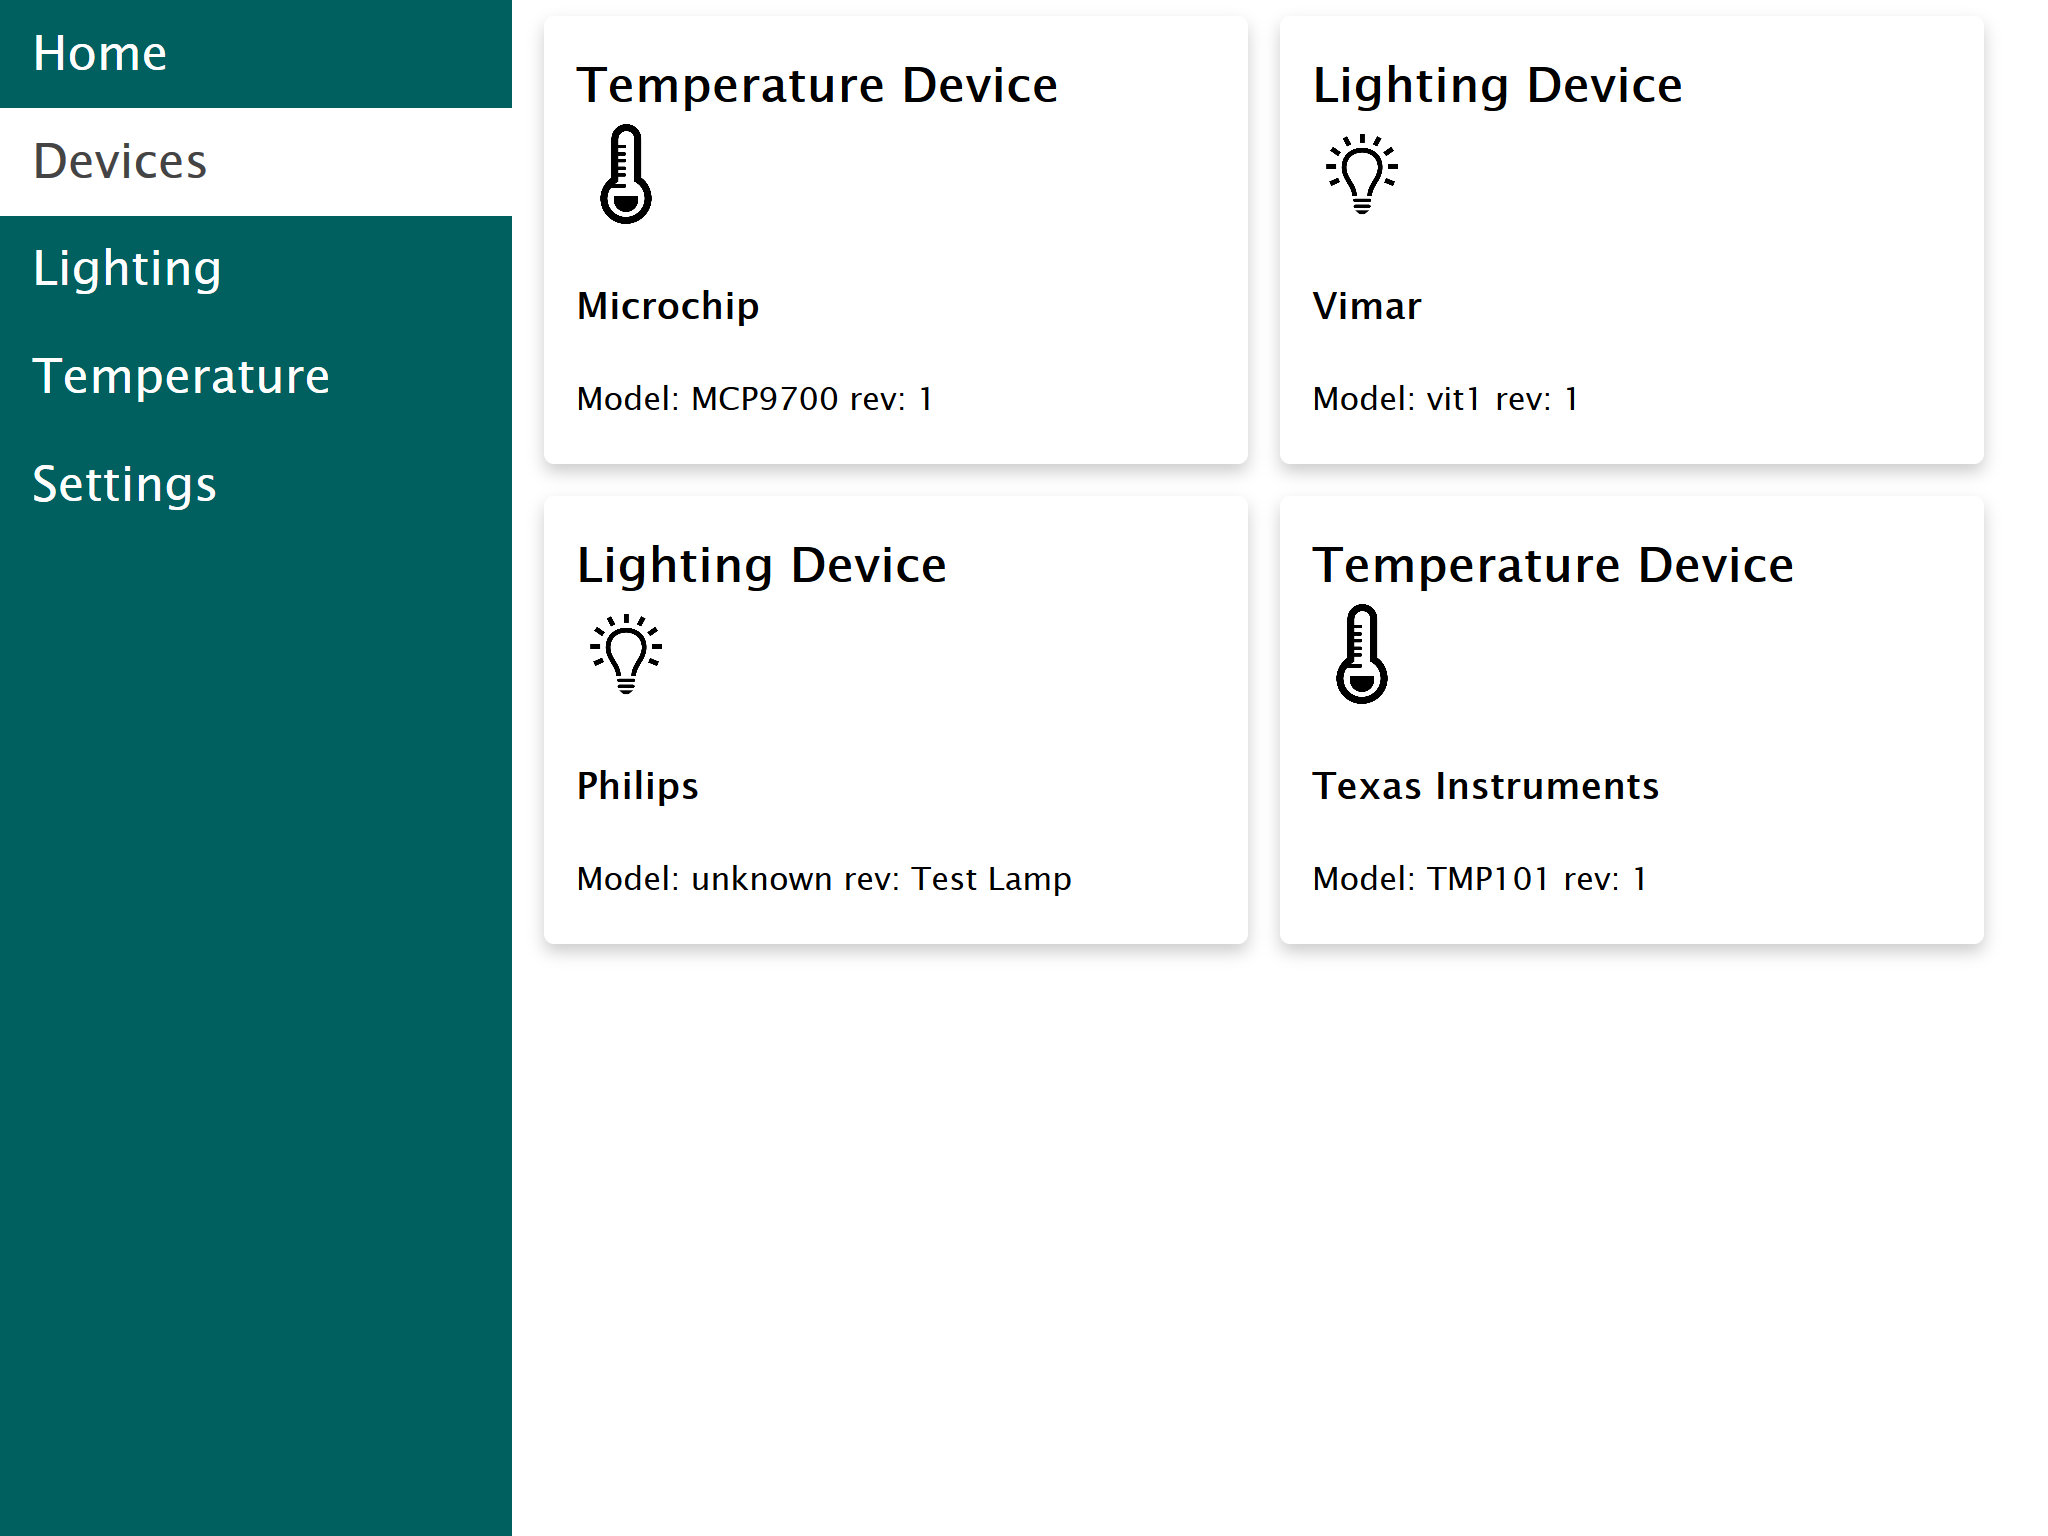
\includegraphics[width=0.9\columnwidth]{demo/devices}
    \caption{Pagina che ricapitola i dispositivi collegati alla \emph{dashboard}}
    \label{fig:devices}
\end{figure}

Nella pagina dedicata alle aree tematiche legate all'illuminazione e alla temperatura, riprendo la visualizzazione mostrata per l'elenco dei dispositivi collegati, mostrando solamente i dispositivi di quella categoria. Nel caso della pagina legata alla temperatura, per ogni dispositivo visualizzo l'identificativo del dispositivo, l'ultima temperatura rilevata e la data in cui il sensore ha misurato quella temperatura. Nella pagina legata all'illuminazione espongo per ogni dispositivo l'identificativo e la data dell'ultima comunicazione con la lampada.
Selezionando uno dei dispositivi elencati, apro una pagina di dettaglio in cui presento le ultime misurazioni disponibili (fino a 50) in un grafico.
Come è possibile osservare in figura ~\ref{fig:temp}, nella pagina di dettaglio di un sensore di temperatura visualizzo il suo identificativo, il produttore, il modello, la revisione e un grafico con l'andamento della temperatura rilevata dal dispositivo.
Ho implementato una funzionalità di personalizzazione dell'unità di misura per la temperatura: l'utente, accedendo alla pagina \emph{Settings}, può scegliere l'unità di misura della temperatura tra quelle gestite dal sistema. Quando l'utente cambia l'unità di misura, questa modifica si ripercuote su tutte le misurazioni di temperatura visualizzabili nella \emph{dashboard}, inclusi i grafici della temperatura.

\begin{figure}[!h]
    \centering
    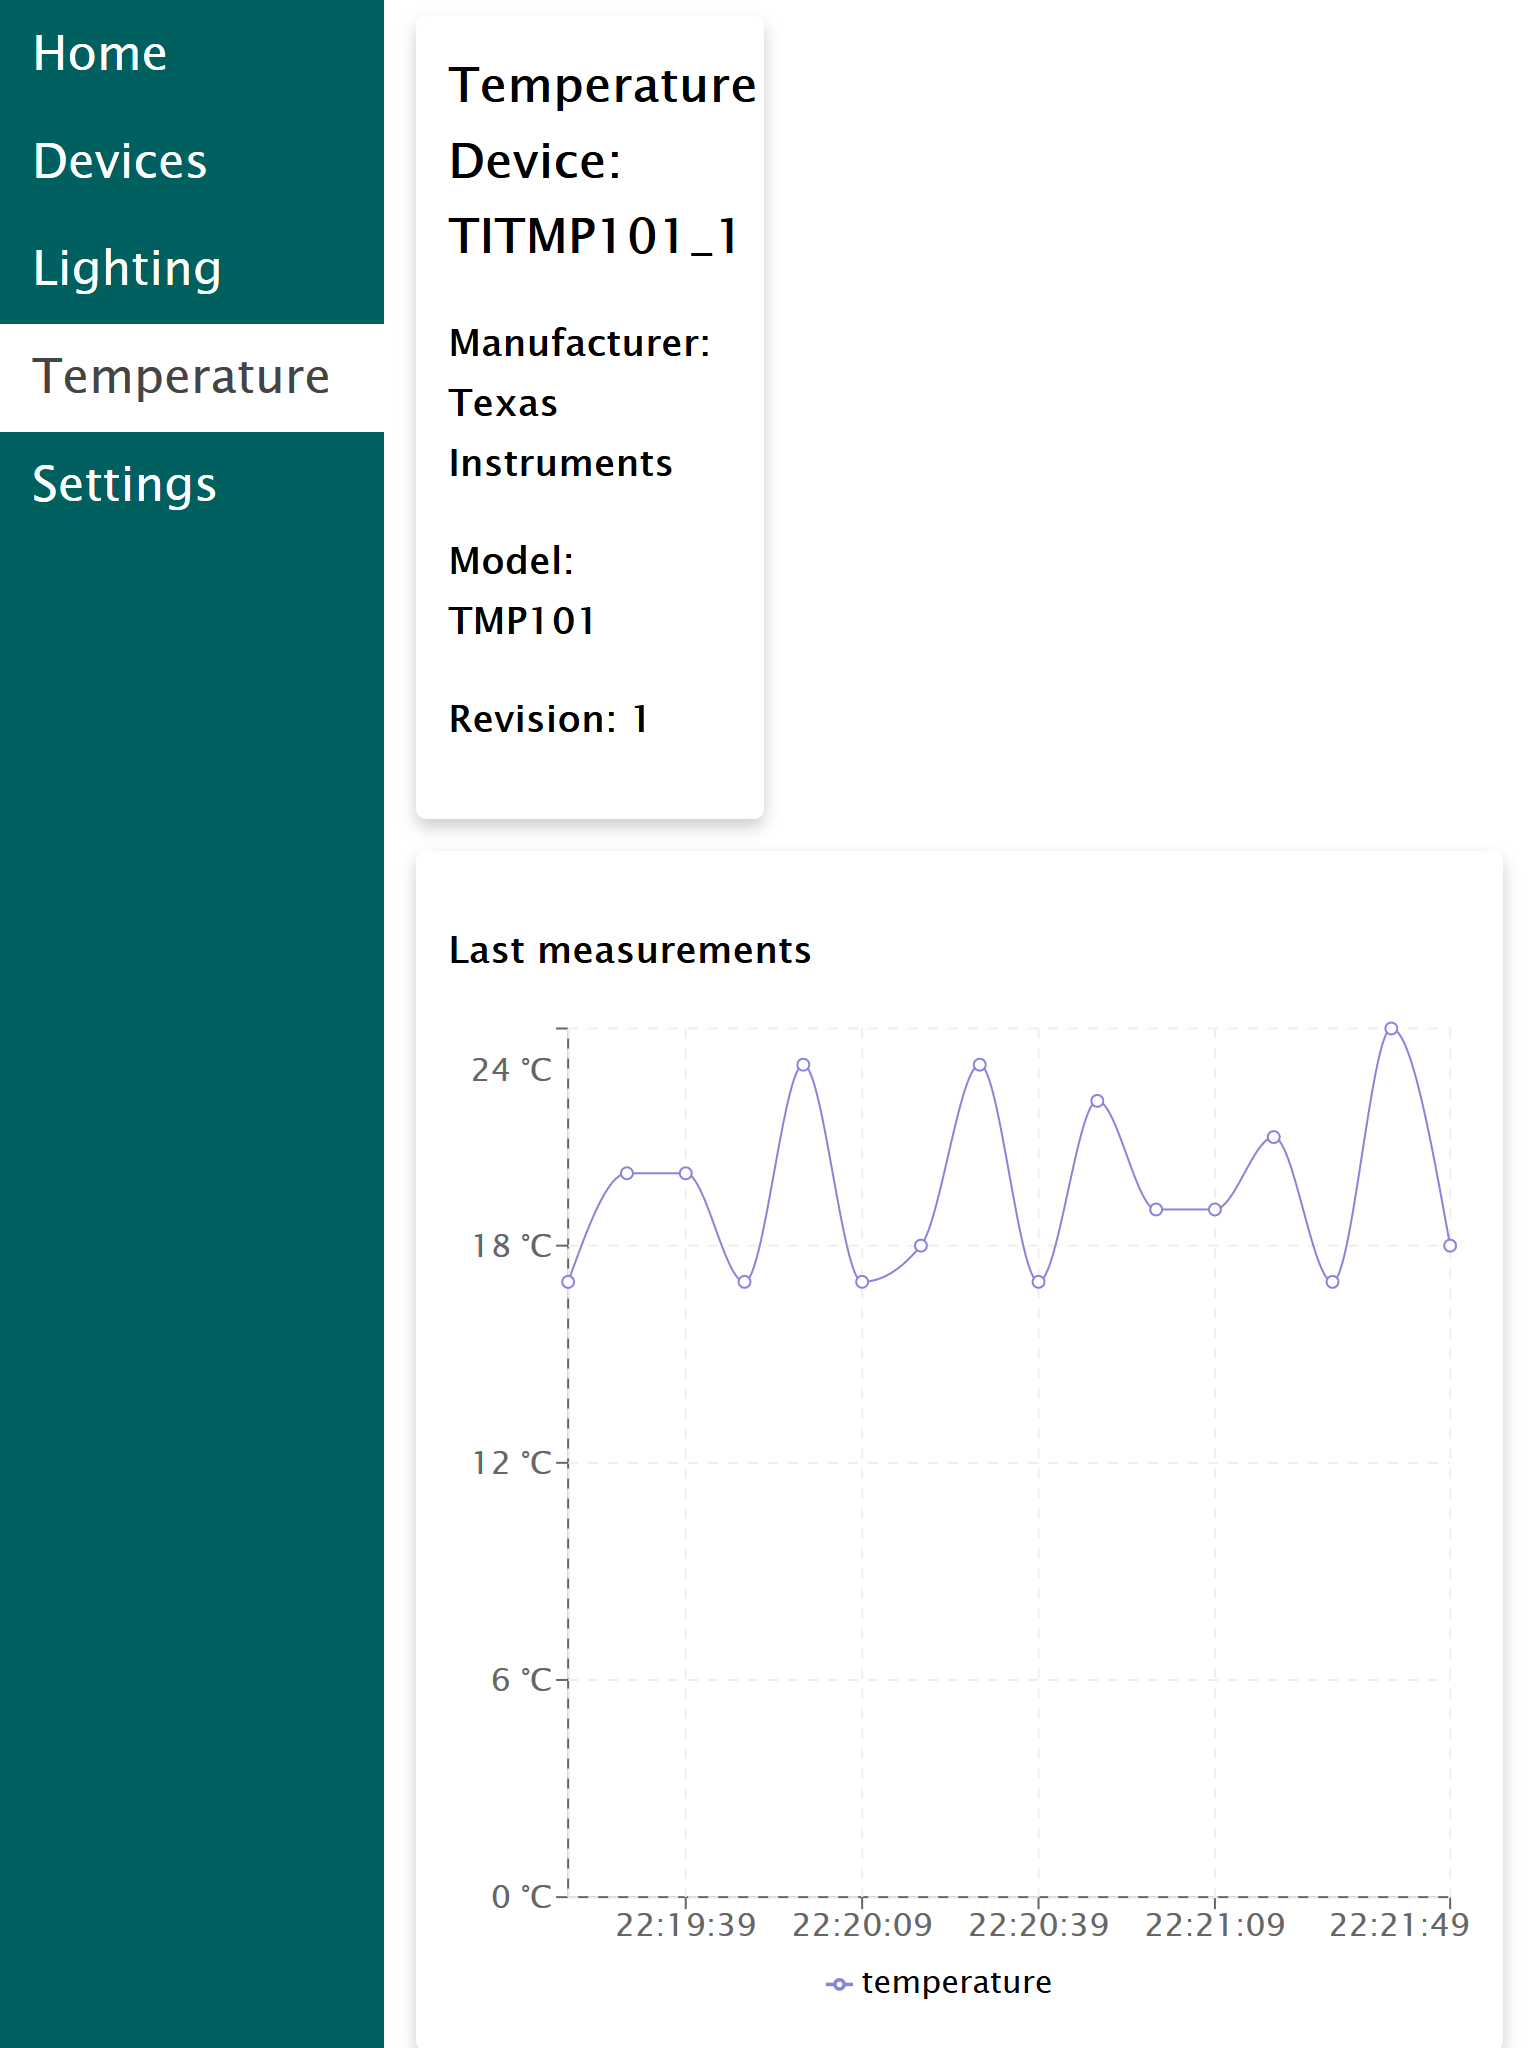
\includegraphics[width=0.6\columnwidth]{demo/ti-temperature}
    \caption{Pagina con il dettaglio di un sensore di temperatura}
    \label{fig:temp}
\end{figure}

Nella pagina di dettaglio delle lampade controllabili da remoto, presento le informazioni già citate con l'aggiunta di un interruttore per l'accensione e lo spegnimento della lampada. In questo caso nel grafico con le misurazioni indico sulle ordinate la potenza assorbita dalla lampada, secondo specifica del dispositivo. Ho incluso in figura ~\ref{fig:light} una schermata della pagine di dettaglio con la lampada spenta e in figura ~\ref{fig:light-on} una schermata della stessa pagina con la lampada accesa.

\begin{figure}[H]
    \centering
    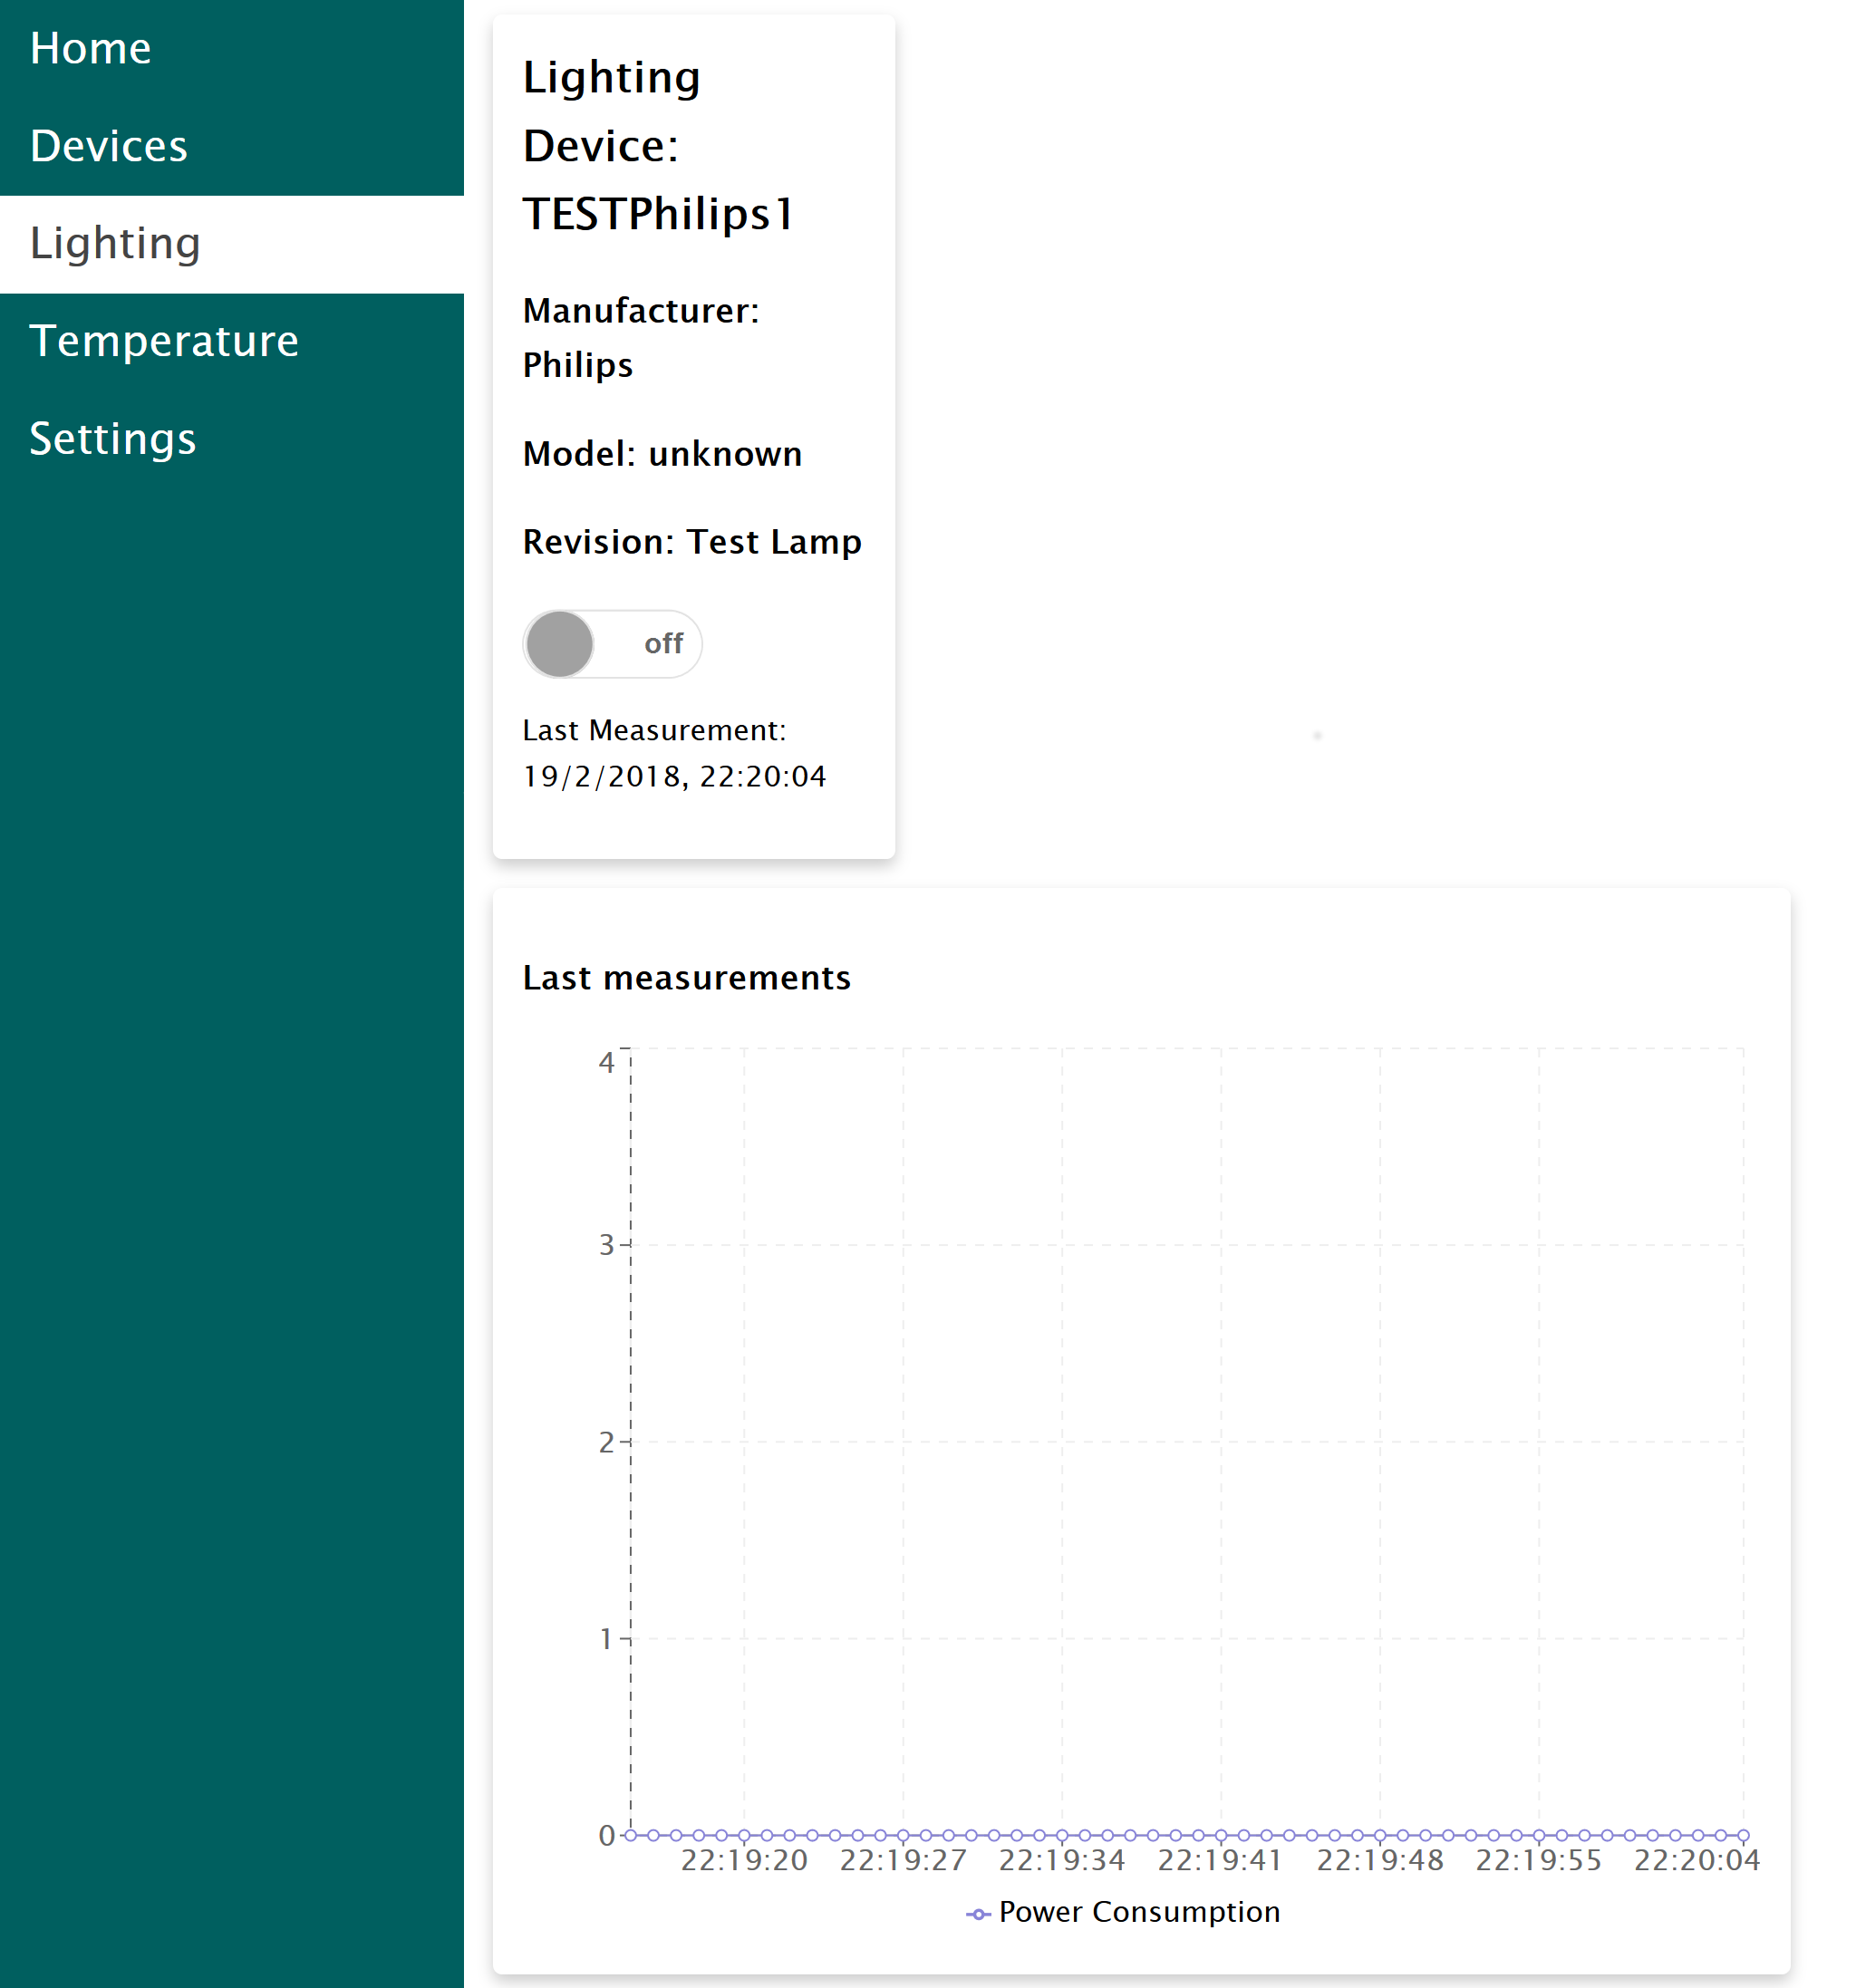
\includegraphics[width=0.6\columnwidth]{demo/philips-light}
    \caption{Pagina di dettaglio della lampada spenta}
    \label{fig:light}
\end{figure}

\begin{figure}[H]
    \centering
    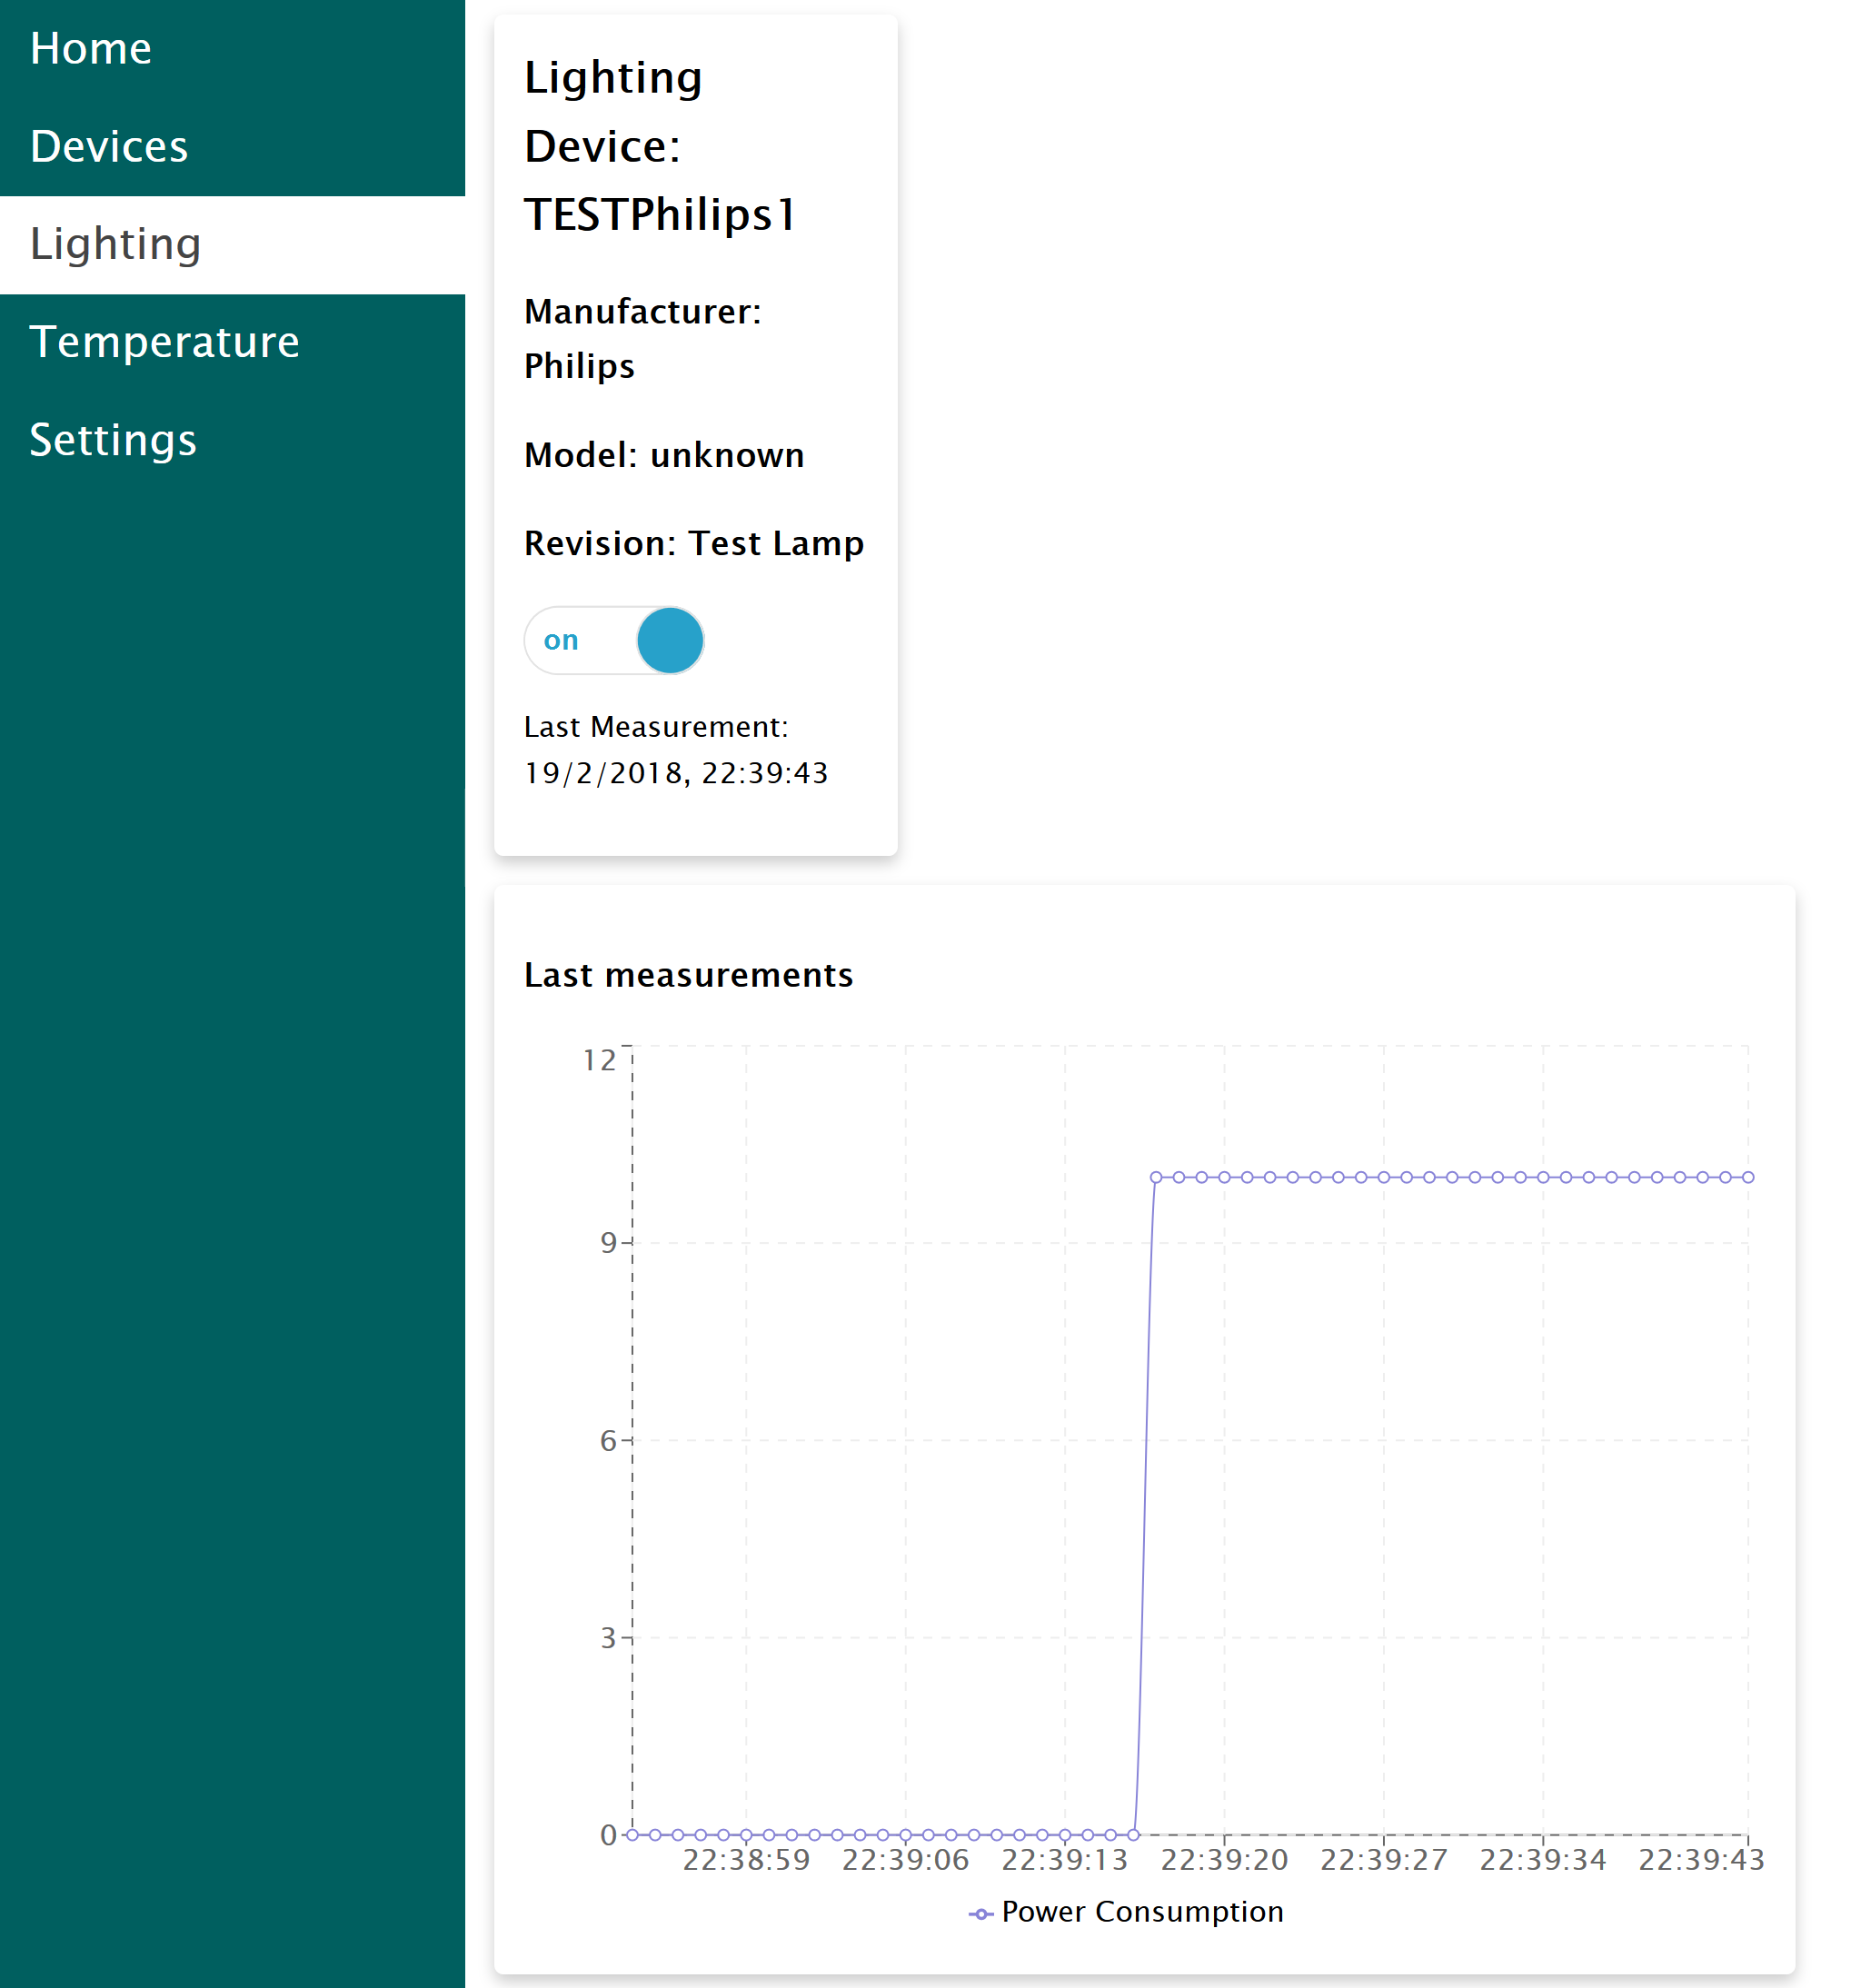
\includegraphics[width=0.6\columnwidth]{demo/philips-light-on}
    \caption{Pagina di dettaglio della lampada accesa}
    \label{fig:light-on}
\end{figure}

\section{Raggiungimento degli obiettivi}

Per valutare correttamente il raggiungimento degli obiettivi è necessario che riprenda gli obiettivi fissati nel capitolo ~\ref{cap:processi-metodologie}.
In particolare voglio osservare le tabelle in cui ho fissato gli obiettivi di prodotto (~\ref{tab:obiettivi-prodotto}), gli obiettivi formativi (~\ref{tab:obiettivi-formativi}) e tecnici (~\ref{tab:obiettivi-tecnici}) del progetto.

Iniziando dalla valutazione degli obiettivi di prodotto, posso definirmi soddisfatto delle funzionalità implementate nel prototipo.
Ho soddisfatto gli obiettivi "OP2" e "OP3", a cui avevo assegnato importanza critica, e quindi il prototipo mostra correttamente quello che mi aspettavo di presentare.
L'utente della \emph{dashboard} del prototipo può visualizzare correttamente la lista di dispositivi collegati al sistema e, per ciascuno di essi, può vedere:
\begin{itemize}
  \item le specifiche generali che comprendono:
  \begin{itemize}
    \item nome del dispositivo;
    \item produttore del dispositivo;
    \item revisione del dispositivo;
  \end{itemize}
  \item le ultime misurazioni provenienti dal dispositivo, nell'unità di misura scelta dall'utente;
  \item se il dispositivo presenta funzionalità \emph{smart}, elementi grafici che permettono all'utente di avviare tali funzionalità.
\end{itemize}
Ho parzialmente implementato le funzionalità descritte negli obiettivi "OP1" e "OP5".
Per quanto riguarda "OP1", nella pagina principale della \emph{dashboard} l'utente può osservare lo stato dei servizi che compongono il sistema, tuttavia considero questo obiettivo solamente parzialmente soddisfatto perché mi aspettavo di riuscire a visualizzare maggiori informazioni, come ad esempio le statistiche del traffico dati all'interno della rete.
Per quanto riguarda "OP5", l'utente può accedere a una pagina in cui può solamente cambiare due opzioni:
\begin{itemize}
  \item il proprio nome nel sistema;
  \item l'unità di misura della temperatura, utile nella visualizzazione delle temperature rilevate dai dispositivi legati a questo ambito.
\end{itemize}
Considero l'obiettivo "OP5" solamente parzialmente soddisfatto in quanto all'inizio del progetto mi aspettavo di riuscire a includere più opzioni di personalizzazione per l'utente.
L'omissione dell'obiettivo "OP4" e la parziale implmentazione di "OP5" e "OP1" è stata causata da due fattori:
\begin{itemize}
  \item difficoltà nelle attività di implementazione, citate in ~\ref{val-req};
  \item sottovalutazione dell'impegno richiesto per implementare le funzionalità più importanti.
\end{itemize}
Considero che le difficoltà implementative che ho riscontrato siano state causate dalla mia inesperienza con la realizzazione di architetture \emph{software} distribuite e dalla mancanza di documentazione che illustri le \emph{best practice} applicate in sistemi reali.
Nella tabella ~\ref{tab:esito-obiettivi-prodotto} riassumo la valutazione degli obiettivi di prodotto soddisfatti.

\begin{table}[H]
\caption{Tabella di valutazione delle funzionalità implementate nel prototipo}
\label{tab:esito-obiettivi-prodotto}
\begin{tabularx}{\linewidth}{|c|X|c|}
\hline
\textbf{Id obiettivo} & \textbf{Descrizione obiettivo} & \textbf{Esito}\\
\hline
OP1 & Visualizzare lo stato generale del sistema. & Parzialmente soddisfatto \\
\hline
OP2 & Visualizzare quali dispositivi sono collegati al sistema. & Soddisfatto \\
\hline
OP3 & Visualizzare le informazioni trasmesse dai dispositivi collegati al sistema. & Soddisfatto \\
\hline
OP4 & Implementare sistemi di autenticazione dell'utente. & Omesso \\
\hline
OP5 & Visualizzare e gestire le preferenze dell'utente. & Parzialmente soddisfatto \\
\hline
\end{tabularx}
\end{table}

Ho inserito nella tabella ~\ref{tab:esito-obiettivi-formativi} la mia valutazione degli obiettivi formativi del progetto.
Considero l'obiettivo "OF1" soddisfatto in quanto le attività di analisi svolte mi hanno permesso di individuare le funzionalità di dispositivi IoT che corrispondono a prodotti esistenti, confermando di fatto che le funzionalità che ho individuato sono richieste dal mercato.
Considero l'obiettivo "OF2" soddisfatto in quanto durante le attività di analisi ho individuato quali caratteristiche di prestazioni e affidabilità sono richieste da dispositivi con risorse di elaborazione limitate ed ho associato queste caratteristiche a ciascun protocollo valutato per determinare quale soluzione tecnica adottare. Ho quindi imparato a valutare l'importanza delle tecniche di individuazione e correzione degli errori dal punto di vista \emph{software}, della gestione dell'instaurazione del collegamento tra i dispositivi e della quantità di informazioni aggiuntive necessarie per la comunicazione delle informazioni.
Considero l'obiettivo "OF3" parzialmente soddisfatto in quanto durante l'esperienza di sviluppo del progetto di stage non sono riuscito ad approfondire gli aspetti meno documentati delle architetture a microservizi; nonostante ciò, ho comunque sviluppato un'architettura a microservizi scalabile, nella quale ho sperimentato personalmente i pregi e i difetti di una simile architettura.
Considero l'obiettivo "OF4" soddisfatto in quanto fin dalle prime attività di progettazione e implementazione ho utlizzato \emph{container} per isolare i microservizi realizzati; inoltre grazie alle difficoltà incontrate durante lo sviluppo riguardanti la comunicazione tra i servizi, ho approdondito le problematiche legate alla visibilità dei servizi nel contesto di reti parzialmente isolate, in cui le comunicazioni sono regolamentate da un entità che non permette una comunicazione indiscriminata tra \emph{container}, ma richiede la definizione di quali \emph{container} nella rete sono visibili, in gergo tecnico "reperibili" (\emph{discoverable}).

\begin{table}[H]
\caption{Tabella di valutazione degli obiettivi formativi del progetto}
\label{tab:esito-obiettivi-formativi}
\begin{tabularx}{\linewidth}{|c|X|c|}
\hline
\textbf{Id obiettivo} & \textbf{Descrizione obiettivo} & \textbf{Esito}\\
\hline
OF1 & Apprendere abilità elementari per la comprensione delle funzionalità richieste dal mercato IoT, specialmente nel campo della automazione domestica. & Soddisfatto \\
\hline
OF2 & Acquisire conoscenze adeguate alla scelta e implementazione di un protocollo di comunicazione adeguato al campo di utilizzo del progetto. & Soddisfatto \\
\hline
OF3 & Comprendere il concetto di architettura a microservizi, con i pregi e i difetti caratteristici di una tale architettura. & Parzialmente soddisfatto \\
\hline
OF4 & Acquisire le nozioni legate alla containerizzazione di un sistema \emph{software} in un contesto architetturale basato su microservizi. & Soddisfatto \\
\hline
\end{tabularx}
\end{table}

Nella tabella ~\ref{tab:esito-obiettivi-tecnici} ho inserito l'esito della valutazione degli obiettivi tecnici del progetto.
Considero gli obiettivi "OT1" e "OT2" totalmente soddisfatti in quanto ho rilasciato il codice sorgente del prototipo su un \emph{repository} GitHub (\url{https://github.com/niktekusho/IoTDashboard}), nel quale ho indicato i requisiti \emph{software} per l'esecuzione del progetto e le istruzioni per eseguire il progetto dopo aver installato i requisiti. Inoltre per ogni servizio ho riportato le istruzioni per provare le funzionalità del servizio in totale isolamento dagli altri servizi che compongono il sistema.
Considero l'obiettivo "OT3" parzialmente soddisfatto in quanto ho realizzato il sistema in modo che i servizi siano eseguibili su diversi dispositivi, tuttavia nello sviluppo non ho implementato dispositivi reali che funzionino come sensori, in quanto fuori dalle responsabilità del progetto.
Considero l'obiettivo "OT4" completamente soddisfatto in quanto su un singolo elaboratore è possibile testare le funzionalità del sistema in una rete comprendente un numero variabile di dispositivi, implementati come sensori di temperatura con specifiche diverse e lampade \emph{smart} controllabili da remoto.
Considero l'obiettivo "OT5" parzialmente soddisfatto perché non ho implementato direttamente strumenti per gestire la scalabilità dei servizi, ma mi sono appoggiato agli strumenti messi a disposizione da Docker Compose per definire le regole di scalabilità dei servizi. Attraverso queste regole, Docker mi ha permesso di aggiungere istanze dei servizi in base alla quantità di richieste che il sistema deve gestire e nel caso di malfunzionamenti di uno o più servizi di riavviarli fino a tre volte in cinque minuti prima di interromperli del tutto.
Ho soddisfatto gli obiettivi "OT6" e "OT7" in quanto ho implementato i servizi con le tecnologie che ho pianificato di usare: Node.js per i servizi di gestione della temperatura, dell'illuminazione, delle informazioni dei dispositivi, delle preferenze utente e per il servizio di interfacciamento tra \emph{client} e i microservizi precedenti e React per la realizzazione dell'applicazione \emph{web}.

\begin{table}[H]
\caption{Tabella di valutazione degli obiettivi tecnici del progetto}
\label{tab:esito-obiettivi-tecnici}
\begin{tabularx}{\linewidth}{|c|X|c|}
\hline
\textbf{Id obiettivo} & \textbf{Descrizione obiettivo} & \textbf{Esito}\\
\hline
OT1 & Rilascio del codice sorgente del prototipo e della documentazione associata nei termini di una licenza \gls{open source}. & Soddisfatto \\
\hline
OT2 & La documentazione associata al progetto deve includere le istruzioni necessarie all'esecuzione del prototipo. & Soddisfatto \\
\hline
OT3 & Il prototipo deve essere eseguibile su dispositivi presenti in una rete, previa corretta configurazione. & Parzialmente soddisfatto \\
\hline
OT4 & Il prototipo deve essere eseguibile su un dispositivo di test, che simuli l'esecuzione in un ambiente reale. & Soddisfatto \\
\hline
OT5 & Il prototipo deve prevedere strumenti per gestire la scalabilità del sistema e per monitorarne lo stato. & Parzialmente soddisfatto \\
\hline
OT6 & Il prototipo deve essere implementato in \href{https://nodejs.org/en/about/}{Node.js} (\url{https://nodejs.org/en/about/}) per il lato server. & Soddisfatto \\
\hline
OT7 & L'interfaccia utente del prototipo deve essere implementata in \href{https://reactjs.org/}{React} (\url{https://reactjs.org/}). & Soddisfatto \\
\hline
\end{tabularx}
\end{table}


%**************************************************************
\section{Conoscenze acquisite}

Durante lo svolgimento del progetto di stage ho studiato e approfondito alcune tecnologie di cui avevo conoscenza e altre che mi erano completamente sconosciute.

Valuto di seguito l'esperienza che ho avuto con le tecnologie e gli strumenti di cui avevo conoscenza pregressa:
\begin{itemize}
  \item \textbf{Node.js}: dal momento che Node.js utilizza il modello \emph{event-driven} per la gestione delle operazioni di \emph{input} e \emph{output} ho semplificato molto la gestione asincrona delle richieste concorrenti. Tra gli aspetti negativi ho osservato che Node.js favorisce attivamente l'utilizzo del Design Pattern \gls{callback}, inducendo alla scrittura di codice sorgente eccessivamente complesso. Considero questo difetto poco rilevante dal momento che Node.js, nella versione \texttt{9.3.0} che ho utilizzato per il progetto, supporta la sintassi definita in ECMAScript 2017 per la definizione di funzioni asincrone senza l'utilizzo del \emph{pattern} \emph{callback}. Grazie alle \emph{keyword} \texttt{async} e \texttt{await}, ho implementato funzioni asincrone, leggibili dagli sviluppatori come se fossero istruzioni sequenziali, evitando un'eccessiva complessità del codice.
  \item \textbf{React}: la natura a componenti che React cerca di diffondere mi ha permesso di riutilizzare molte componenti grafiche, aumentando la mia  produttività e garantendo una maggiore affidabilità delle componenti. Dal momento che i dati di una componente figlia non possono modificare direttamente i dati di una componente padre ho riscontrato che le attività di manutenzione delle componenti è stata semplice, permettendomi di identificare in breve tempo eventuali errori nel codice.
  \item \textbf{Jest}: durante il suo utilizzo ho osservato che è una piattaforma di test completa, che include strumenti di validazione dei risultati e strumenti per il \gls{mocking}, e che non richiede una configurazione da parte dell'utente, utilizzando impostazioni predefinite ottimali. Un altro aspetto che ho osservato durante le attività di codifica è che i test scritti vengono eseguiti in parallelo, velocizzando di molto l'individuazione di errori nel codice. Un aspetto negativo che ho riscontrato in Jest consiste nella sua minore flessibilità rispetto ad altre librerie di test, le quali permettono ad esempio di sostituire le componenti di valutazione delle istruzioni. Nell'ambito del progetto di stage non ho trovato questo difetto rilevante, tuttavia con diverse esigenze una maggiore flessibilità potrebbe essere richiesta.
  \item \textbf{ESLint}: ho trovato questo strumento fondamentale durante le attività di codifica in quanto, attraverso la definizione di regole comuni per la scrittura del codice sorgente del progetto, mi ha permesso di scrivere codice sorgente con uno stile uniforme e mi ha segnalato preventivamente possibili errori nel codice scritto. L'integrazione con l'\emph{editor} di testo ha migliorato la mia produttività, permettendomi di non lasciare mai l'ambiente di scrittura per controllare la validità del codice prodotto. Un altro aspetto che ho apprezzato riguarda la semplicità con cui ho individuato le soluzioni agli errori segnalati dallo strumento, grazie alla sua documentazione ben realizzata. L'aspetto negativo principale che ho rilevato consiste nella necessità di creare un \emph{file} di configurazione in cui la definizione delle regole, pur essendo ben documentata, richiede una quantità di tempo non banale. Durante il progetto sono riuscito a mitigare questo difetto utilizzando un \emph{template} comune per la generazione dei servizi.
  \item \textbf{HTML5}: del linguaggio HTML5 ho apprezzato subito la sintassi semplificata e più chiara rispetto alle versioni precedenti dello standard; inoltre essendo ormai supportato da tutti i \emph{browser} sul mercato non ho trovato difficoltà a rendere multipiattaforma l'interfaccia \emph{web} della \emph{dashboard}. Un altro aspetto che ha aumentato il mio grado di soddisfazione riguardo a questo linguaggio risiede nella facilità con cui si trovano in rete risorse che spieghino come utilizzare in maniera ottimale le funzionalità del linguaggio.
  \item \textbf{Docker Engine}: ho constatato che la gestione del ciclo di vita di un \emph{container} per mezzo del Docker Engine è molto semplice ed intuitiva, grazie alla buona documentazione per l'utilizzo; ho trovato che la creazione di \emph{container} basati su una stessa formula è molto semplice e ben documentata attraverso la creazione di \emph{file} \emph{Dockerfile}, nei quali ho specificato il sistema operativo del \emph{container}, le dipendenze necessarie all'esecuzione del servizio e quali risorse il servizio espone.
  \item \textbf{Atom}: è l'\emph{editor} che ho utilizzato per scrivere la documentazione del progetto e ho notato fin da subito che è estremamente personalizzabile, sia in termini di interfaccia grafica sia in termini di supporto alla scrittura, tuttavia mi sono imbattuto in numerose piccole interruzioni nel funzionamento dell'applicazione, dovuti alla quantità di risorse che il \emph{software} allocava. L'aspetto principale che mi ha spinto ad utilizzare un altro strumento per la codifica risiede nell'assenza di un'integrazione nativa con gli strumenti di \emph{debug} del codice.
\end{itemize}

Valuto di seguito l'esperienza che ho avuto con le tecnologie e gli strumenti che ho introdotto per lo sviluppo del prototipo:
\begin{itemize}
  \item \textbf{ECMAScript 2017}: della nuova versione dello standard ho apprezzato la nuova sintassi per la scrittura di funzioni asincrone e la modifica di poche caratteristiche del linguaggio. La nuova sintassi per la scrittura di funzioni asincrone ricorda l'utilizzo di normali funzioni della programmazione sequenziale e mi ha permesso di velocizzare l'implementazione delle funzionalità asincrone all'interno del sistema. La quantità limitata di nuove funzionalità rispetto alle edizioni esistenti mi ha consentito di concentrare lo studio al fine di imparare le nuove funzionalità con maggior semplicità. I difetti che ho evidenziato durante lo sviluppo sono due:
  \begin{itemize}
    \item con la nuova sintassi per le funzioni asincrone ho spesso dimenticato la natura asincrona del codice scritto, causando l'omissione della \emph{keyword} \emph{await}. Questa mancanza mi è stata puntualmente evidenziata dagli strumenti di analisi statica che ho scelto di utilizzare, quindi a mio avviso non è stata particolarmente rilevante;
    \item il supporto alla nuova edizione dello standard è presente in maniera completa solamente nelle ultime versioni dei \emph{browser} e di Node.js.\footnotemark
  \end{itemize}
  \item \textbf{CSS3}: dato l'ambito di utilizzo molto limitato all'interno del progetto ho potuto utilizzare poche funzionalità che mi permettessero di valutare pregi e difetti del CSS3. Durante l'implementazione dell'interfaccia grafica ho apprezzato molto la buona documentazione presente in rete sulle funzionalità che ho utilizzato e, unito alla quantità di risorse disponibili in rete, ho implementato velocemente uno stile moderno per l'interfaccia grafica.
  \item \textbf{Visual Studio Code}: reputo questo strumento una delle sorprese positive nell'insieme delle tecnologie e strumenti che ho utilizzato. Ho rilevato che l'\emph{editor} è molto reattivo ed efficiente nell'utilizzo delle risorse, garantendo un'esperienza di utilizzo piacevole. Un altro aspetto positivo che ho apprezzato durante le attività di codifica risiede nel supporto nativo per gli strumenti di \emph{debug} che mi ha permesso di correggere errori introdotti nel codice velocemente. Confrontando Visual Studio Code con l'altro \emph{editor} Atom, posso evidenziare che la quantità di personalizzazioni disponibili è minore nell'\emph{editor} di Microsoft, sia dal punto di vista delle sintassi supportate sia da un punto di vista di personalizzazione generale.
  \item \textbf{Docker Compose}: a mio avviso una delle sorprese negative nell'insieme delle tecnologie e strumenti utilizzati. Da un punto di vista funzionale, ho osservato che Docker Compose offre strumenti di gestione dei \emph{container} intuitivi e non ho incontrato malfunzionamenti imputabili allo strumento. Il lato negativo che ha causato ritardi nell'implementazione dei servizi riguarda la documentazione fornita da Docker: la documentazione fornita è orientata alla parte teorica dello strumento, trascurando la parte pratica che non ho apprezzato in quanto limitata in estensione e contenuti. Un altro aspetto relativo alla documentazione che mi ha confuso quando la ho consultata riguarda la quantità di versioni di Docker Compose attualmente supportate: Docker Compose supporta funzionalità diverse in base alla sua versione e questo si riflette nella quantità troppo ampia di sintassi supportate per la definizione dei servizi.
\end{itemize}

\footnotetext{
\begin{itemize}
	\item[] Tabella di compatiblità dei \emph{browser}: \url{http://kangax.github.io/compat-table/es2016plus/}
	\item[] Tabella di compatiblità di Node.js: \url{http://node.green/\#ES2017}
\end{itemize}}


%**************************************************************
\section{Conclusioni}

Le conoscenze che ho acquisito durante lo svolgimento del progetto di stage mi hanno permesso di espandere i contenuti studiati durante il corso di studi soprattutto da tre punti di vista:
\begin{itemize}
  \item \textbf{reti}: lo studio del protocollo MQTT, non trattato nel corso di "Reti e Sicurezza", non mi ha richiesto particolari sforzi, dal momento che tale corso fornisce una solida base a cui attingere per la costruzione di nuove conoscenze;
  \item \textbf{programmazione distribuita}: in questo caso il divario tra le conoscenze acquisite durante il corso di "Programmazione Concorrente e Distribuita" è stato più difficile da colmare. Infatti tale corso alloca la maggior parte delle risorse alla comprensione della concorrenza, trattando l'argomento "Distribuzione" in maniera più superficiale. Un altro aspetto che ha contribuito a distanziare l'esperienza di stage dalle conoscenze acquisite durante il corso risiede nella mia volontà di utilizzare la tecnologia Node.js per l'implementazione del prodotto, dal momento che Node.js non è una tecnologia trattata dal corso.
  \item \textbf{ingegneria del \emph{software}}: malgrado l'impiego dell'architettura a microservizi mi abbia richiesto lo studio di \emph{Design Pattern} specifici, credo che i concetti teorici e pratici appresi durante il corso di "Ingegneria del \emph{Software}" siano stati fondamentali per il completamento del prototipo, a partire dagli strumenti di analisi e progettazione per giungere alle tecniche di gestione della qualità del \emph{software}.
\end{itemize}

L'esperienza di stage mi ha fatto osservare che la condivisione delle conoscenze all'interno di un gruppo di lavoro consente a tutti i membri del gruppo di crescere formativamente; sebbene avessi preventivato il rischio di non avere abbastanza esperienza quando ho valutato l'ipotesi dello svolgimento di uno stage interno individuale, ho comunque realizzato che l'aspetto collaborativo, a cui sono abituato grazie alla mia attività lavorativa in azienda, mi è mancato soprattutto durante le attività di ricerca e analisi. La sopravvalutazione delle mie capacità e la sottovalutazione degli obiettivi che mi ero preposto ha causato quindi un ridimensionamento degli obiettivi, necessario a contenere le attività all'interno del margine di tempo dedicato allo stage.

Sono comunque soddisfatto dell'opportunità che ho avuto, in quanto ho avuto la possibilità di sperimentare la realizzazione di un sistema con architettura a microservizi nell'ambito della domotica.
             % Concept Preview
% % !TEX encoding = UTF-8
% !TEX TS-program = pdflatex
% !TEX root = ../relazione-finale.tex

%**************************************************************
\chapter{Progettazione e codifica}
\label{cap:progettazione-codifica}
%**************************************************************

\intro{Breve introduzione al capitolo}\\

%**************************************************************
\section{Tecnologie e strumenti}
\label{sec:tecnologie-strumenti}

Di seguito viene data una panoramica delle tecnologie e strumenti utilizzati.

\subsection*{Tecnologia 1}
Descrizione Tecnologia 1.

\subsection*{Tecnologia 2}
Descrizione Tecnologia 2

%**************************************************************
\section{Ciclo di vita del software}
\label{sec:ciclo-vita-software}

%**************************************************************
\section{Progettazione}
\label{sec:progettazione}

\subsubsection{Namespace 1} %**************************
Descrizione namespace 1.

\begin{namespacedesc}
    \classdesc{Classe 1}{Descrizione classe 1}
    \classdesc{Classe 2}{Descrizione classe 2}
\end{namespacedesc}


%**************************************************************
\section{Design Pattern utilizzati}

%**************************************************************
\section{Codifica}
             % Product Prototype
% % !TEX encoding = UTF-8
% !TEX TS-program = pdflatex
% !TEX root = ../relazione-finale.tex

%**************************************************************
\chapter{Verifica e validazione}
\label{cap:verifica-validazione}
%**************************************************************             % Product Design Freeze e SOP
% % !TEX encoding = UTF-8
% !TEX TS-program = pdflatex
% !TEX root = ../relazione-finale.tex

%**************************************************************
\chapter{Conclusioni}
\label{cap:conclusioni}
%**************************************************************

%**************************************************************
\section{Consuntivo finale}

%**************************************************************
\section{Raggiungimento degli obiettivi}

%**************************************************************
\section{Conoscenze acquisite}

%**************************************************************
\section{Valutazione personale}
             % Conclusioni
% \appendix
% % !TEX encoding = UTF-8
% !TEX TS-program = pdflatex
% !TEX root = ../relazione-finale.tex

%**************************************************************
\chapter{Appendice A}
%**************************************************************

\epigraph{Citazione}{Autore della citazione}



             % Appendice A

\newpage

%**************************************************************
% Materiale finale
%**************************************************************
\backmatter
\printglossaries
% !TEX encoding = UTF-8
% !TEX TS-program = pdflatex
% !TEX root = ../relazione-finale.tex

%**************************************************************
% Bibliografia
%**************************************************************

\cleardoublepage
\chapter{Bibliografia}

\nocite{*}
% Stampa i riferimenti bibliografici
\printbibliography[heading=subbibliography,title={Riferimenti bibliografici},type=book]

% Stampa i siti web consultati
\printbibliography[heading=subbibliography,title={Siti web consultati},type=online]


\end{document}
